\chapter{Nondeterministic Finite Automata}\label{ch-4}

A nondeterministic finite automaton, abbreviated NDFA, is a
generalization of the deterministic machines that we have studied
in previous chapters. Although nondeterministic machines lack some
of the restrictions imposed on their deterministic cousins, the
class of languages recognized by nondeterministic finite automata
is exactly the same as the class of languages recognized by
deterministic finite automata.  In this sense, the recognition power
of nondeterministic finite automata is equivalent to that of
deterministic finite automata.

In this chapter we will show the correspondence of nondeterministic
finite automata to deterministic finite automata, and we will prove
that both types of machines accept the same class of languages. In
a later section, we will again generalize our computational model
to allow nondeterministic finite automata that make transitions
spontaneously, without an input symbol being processed. It will be
shown that the class of languages recognized by these new machines
is exactly the same as the class of languages recognized by our
first type of nondeterministic finite automata and is thus the same
as the class of languages recognized by deterministic finite automata.

% 4.1 DEFINITIONS AND BASIC THEOREMS
\section{Definitions and Basic Theorems}\label{sec-4.1}

Whereas deterministic finite automata are restricted to having
exactly one transition from a state for each $\mathbf{a} \in \Sigma$, a
nondeterministic finite automaton may have any number of transitions
for a given input symbol, including zero transitions.

When processing an input string, if an NDFA comes to a state from
which there is no transition arc labeled with the next input symbol,
the path through the machine which is being followed is terminated.
Termination can take the place of the ``garbage state'' (a permanent
rejection state) found in many deterministic finite automata, which
is used to reject some strings that are not in the language recognized
by the automaton (the state $s_7$ played this role in Examples 1.11 and
1.9).

\subsection*{Example 4.1}

Let $L=\{w \in \{\pmb{a},\pmb{b},\pmb{c}\}^*|\ \exists y \in \{\pmb{b}\}^* \ni
w = \pmb{a}y\pmb{c}\}$.  We can easily build a nondeterministic finite automaton
that accepts this set of words. One such automaton is displayed in Figure \ref{fig-4.1}.
In this example there are no transitions out of $s_0$ labeled with either
$\pmb{b}$ or $\pmb{c}$, nor are there any transitions from $s_1$ labeled with
$\pmb{a}$. From state $s_2$ there are no transitions at all. This means that if
either $\pmb{b}$ or $\pmb{c}$ is encountered in state $s_0$ or $\pmb{a}$ is
encountered in state $s_1$, or any input letter is encountered once we reach
state $s_2$, the word on the input tape will not be able to follow this
particular path through the machine. Thus, if a word is not fully processed by
the NDFA, it will not be considered accepted (even if the state in which it was
prematurely ``stuck'' was a final state).

% Figure 4.1
\begin{figure}
\centerline{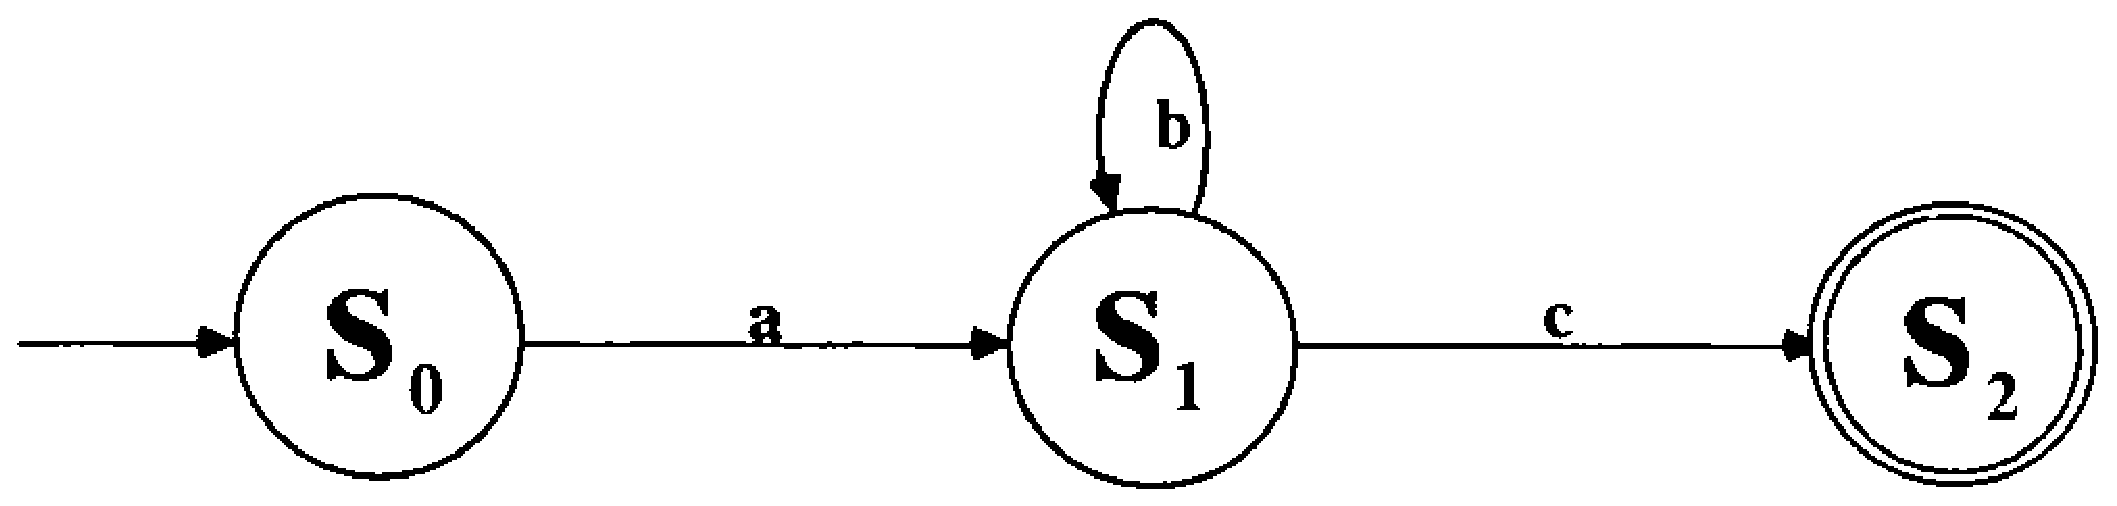
\epsfig{figure=ToFAfigures/fig4-1.eps,width=3in}}
\caption{The NDFA described in Example 4.1}\label{fig-4.1}
\end{figure}

An equivalent, although more complicated, deterministic finite automaton is
given in Figure \ref{fig-4.2}. Note that this deterministic finite automaton requires
the introduction of an extra state, a \emph{\Index{dead state}} or
\emph{\Index{garbage state}}, to continue the processing of strings that are not
in the language.

% Figure 4.2
\begin{figure}
\centerline{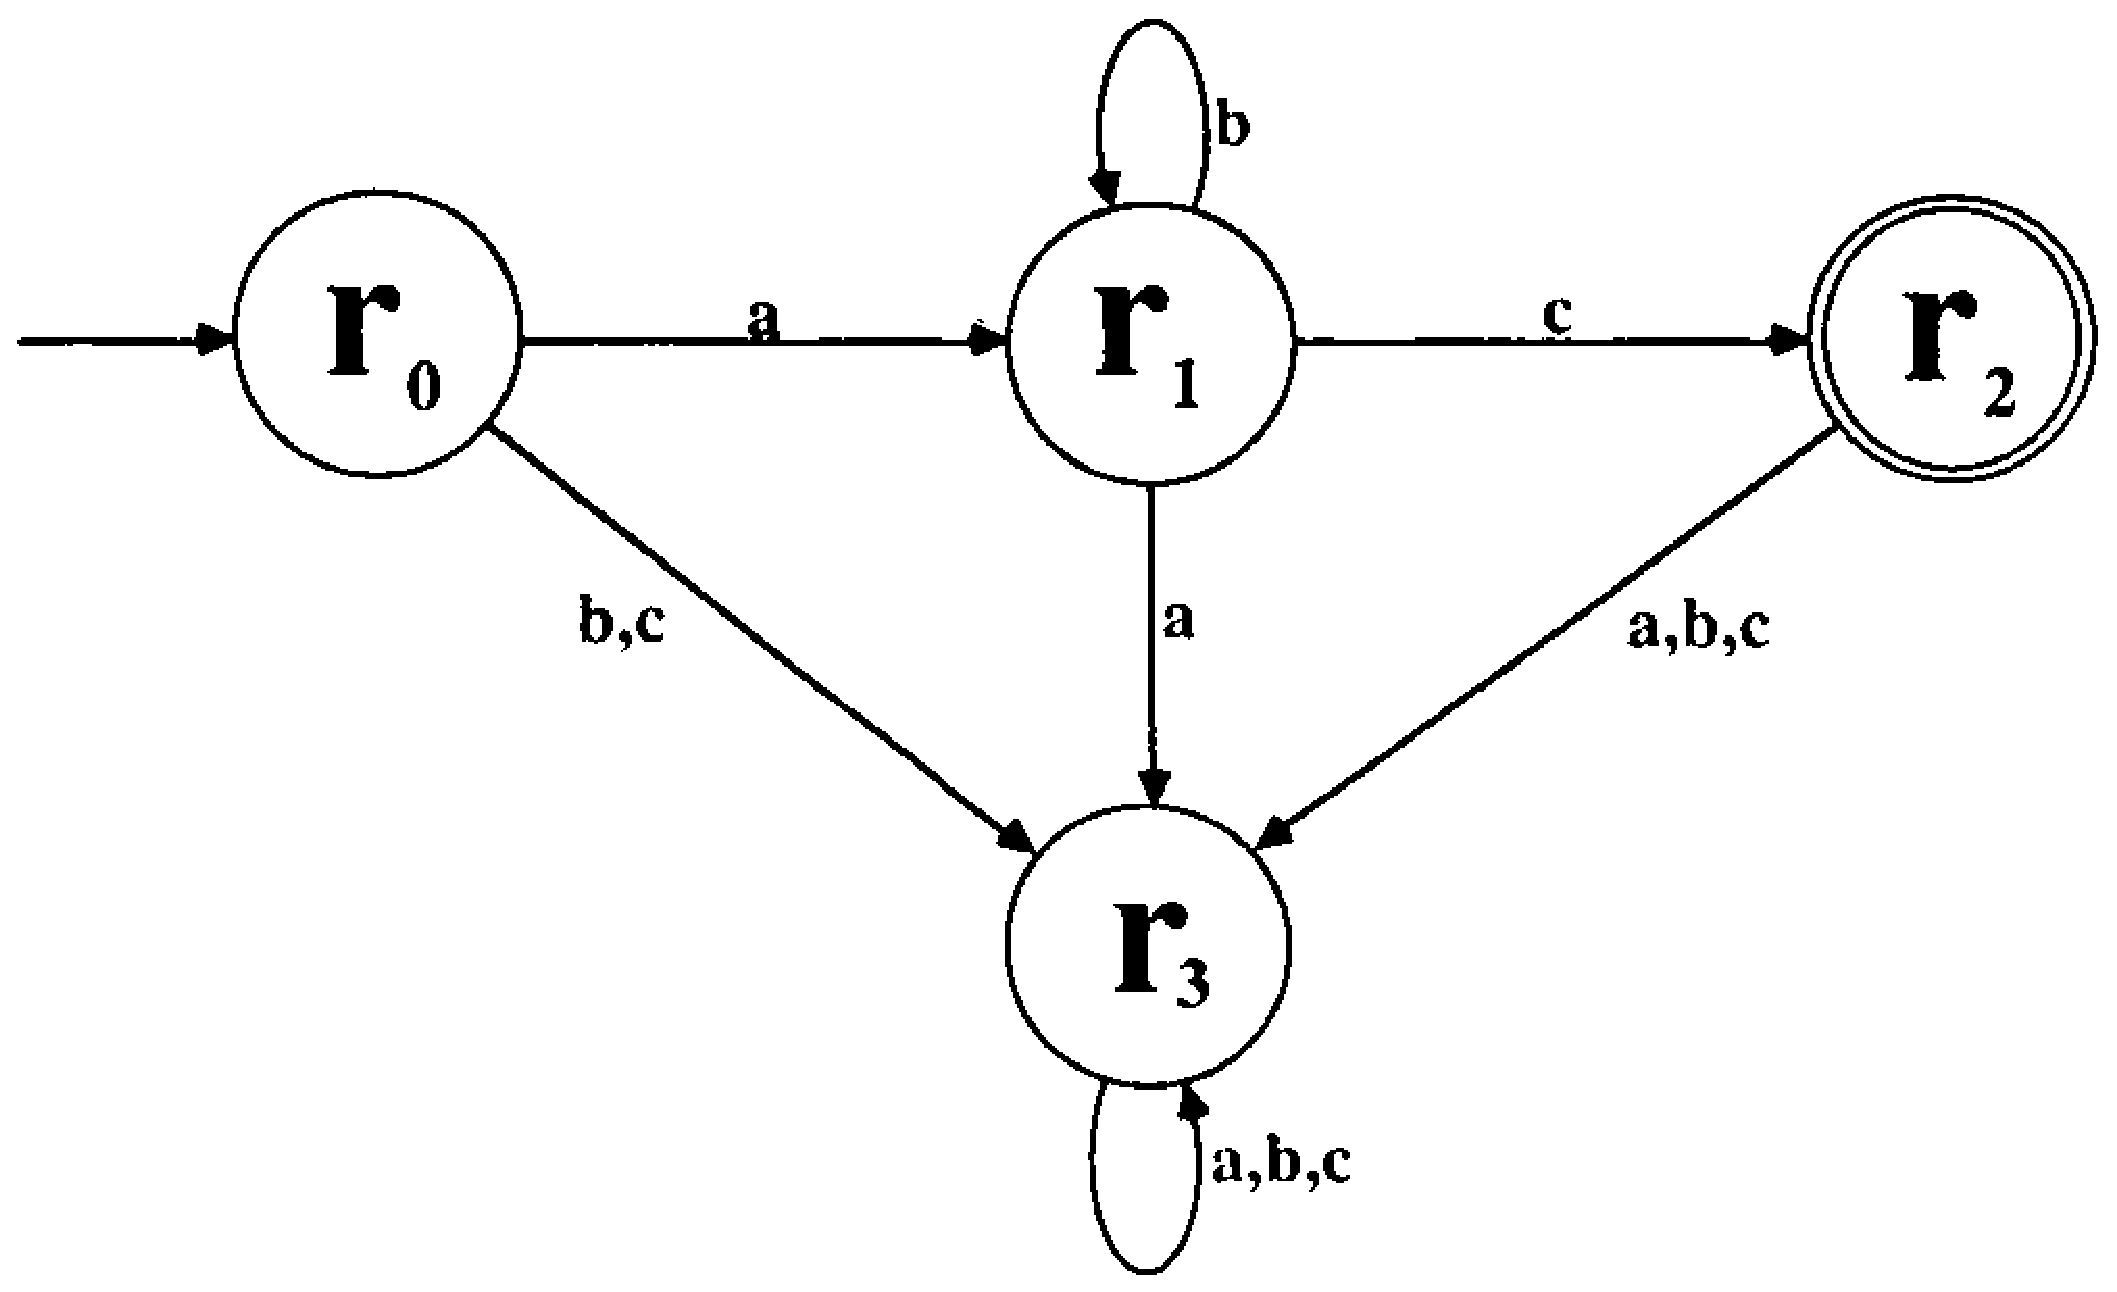
\epsfig{figure=ToFAfigures/fig4-2.eps,width=3in}}
\caption{A deterministic version of the NDFA in Example 4.1}\label{fig-4.2}
\end{figure}

A nondeterministic finite automaton may also have \emph{multiple} transitions
from any state for a given input symbol. For example, consider the following
construction of a nondeterministic acceptor for the language $L$, which consists
of all even-length strings along with all strings whose number of $\pmb{1}$s is
a multiple of 3. That is, $L=\{x \in \{\pmb{0},\pmb{1}\}^*|\ |x| \equiv 0 \bmod{2}
\vee |x|_{\pmb{1}} \equiv 0 \bmod{3}\}$.

\subsection*{Example 4.2}

In the NDFA given in Figure \ref{fig-4.3}, there are multiple transitions from state $s_0$:
processing the symbol $\pmb{0}$ causes the machine to enter states $s_1$ and
$s_2$, whereas processing a $\pmb{1}$ causes the machine to enter both state
$s_3$ and state $s_2$.

% Figure 4.3
\begin{figure}
\centerline{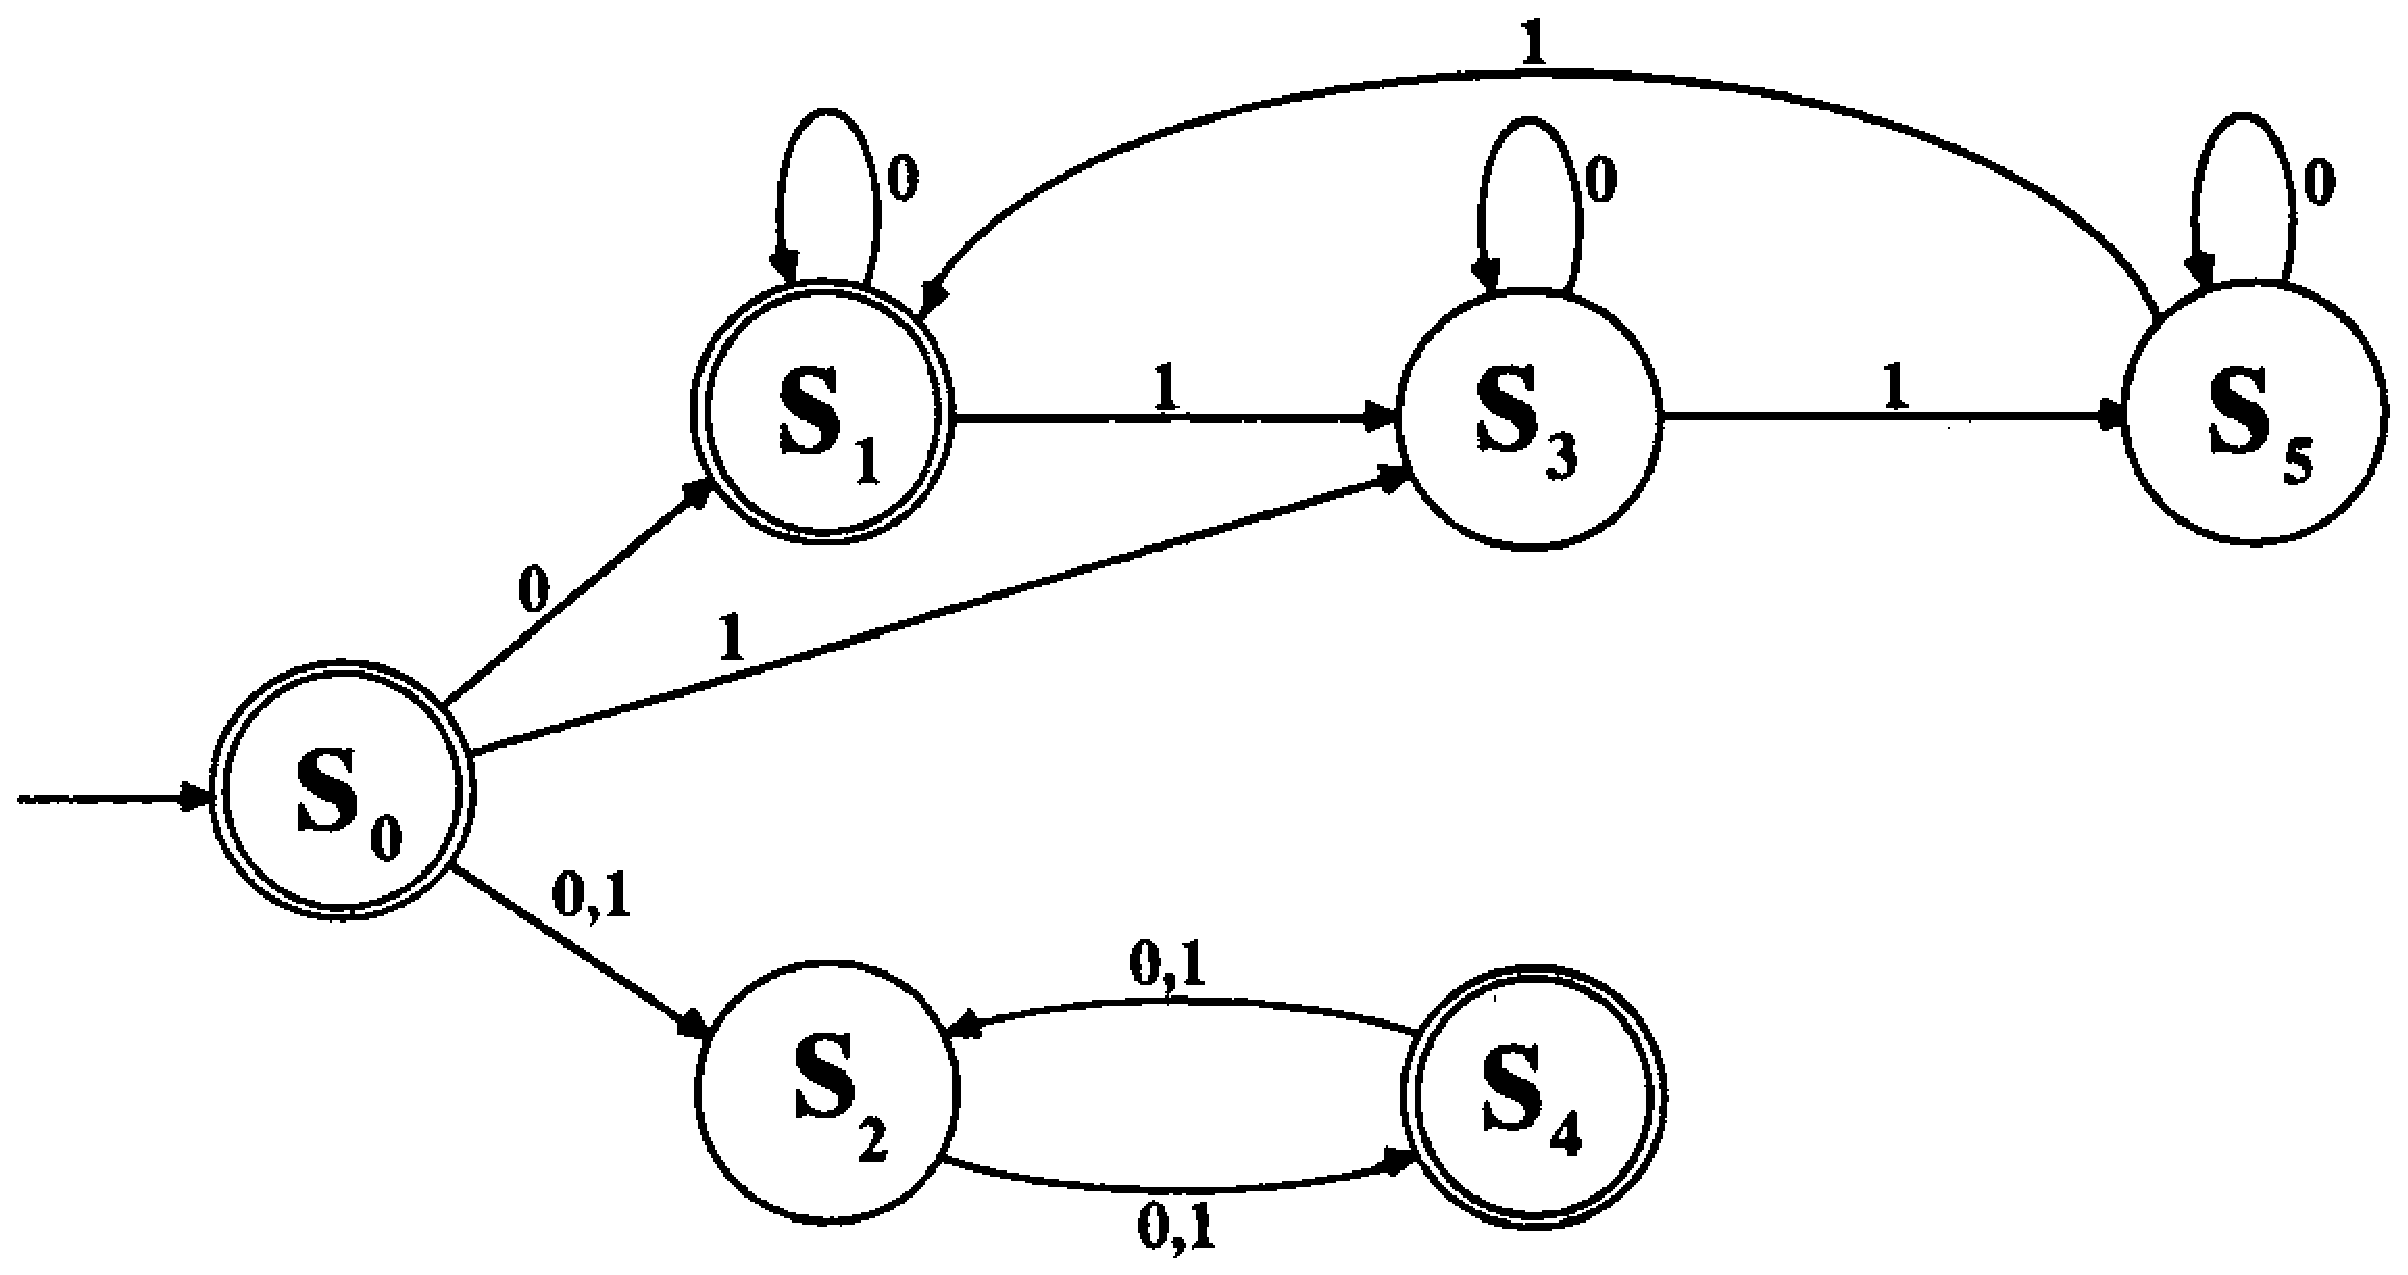
\epsfig{figure=ToFAfigures/fig4-3.eps,width=4in}}
\caption{The NDFA discussed in Example 4.2}\label{fig-4.3}
\end{figure}

Within a nondeterministic finite automaton there can be multiple paths that
are labeled with the components of a string. For example, if we let $w=\pmb{01}$,
then there are two paths labeled by the components of $w:\ (s_0 \rightarrow s_1
\rightarrow s_3)$ and $(s_0 \rightarrow s_2 \rightarrow s_4)$. The second path
leads to a final state, $s_4$, while the first path does not. We will adopt
the convention that this word $w$ \emph{is} accepted by the automaton since at
least one of the paths \emph{does} terminate in a final state. These concepts
will be formalized later in Definition \ref{dfn-4.3}.

This ability to make multiple transitions from a given state can simplify the
construction of the machine, but adds no more power to our computational model.
The deterministic machine equivalent to Example 4.2 is substantially more
complex, and its construction is left as an exercise for the reader.

Another restriction that is relaxed when we talk about nondeterministic finite
automata is the number of initial states. While a deterministic machine is
constrained to having exactly one start state, a nondeterministic finite
automaton may have any number, other than zero, up to $\|S\|$. Indeed, some
applications will be seen in which \emph{all} the states are start states.

\subsection*{Example 4.3}

We can build a machine that will accept the same language as in Example 4.2,
but in a slightly different way. Note that in Figure \ref{fig-4.4} the multiplicity of
start states simplifies the construction considerably.

% Figure 4.4
\begin{figure}
\centerline{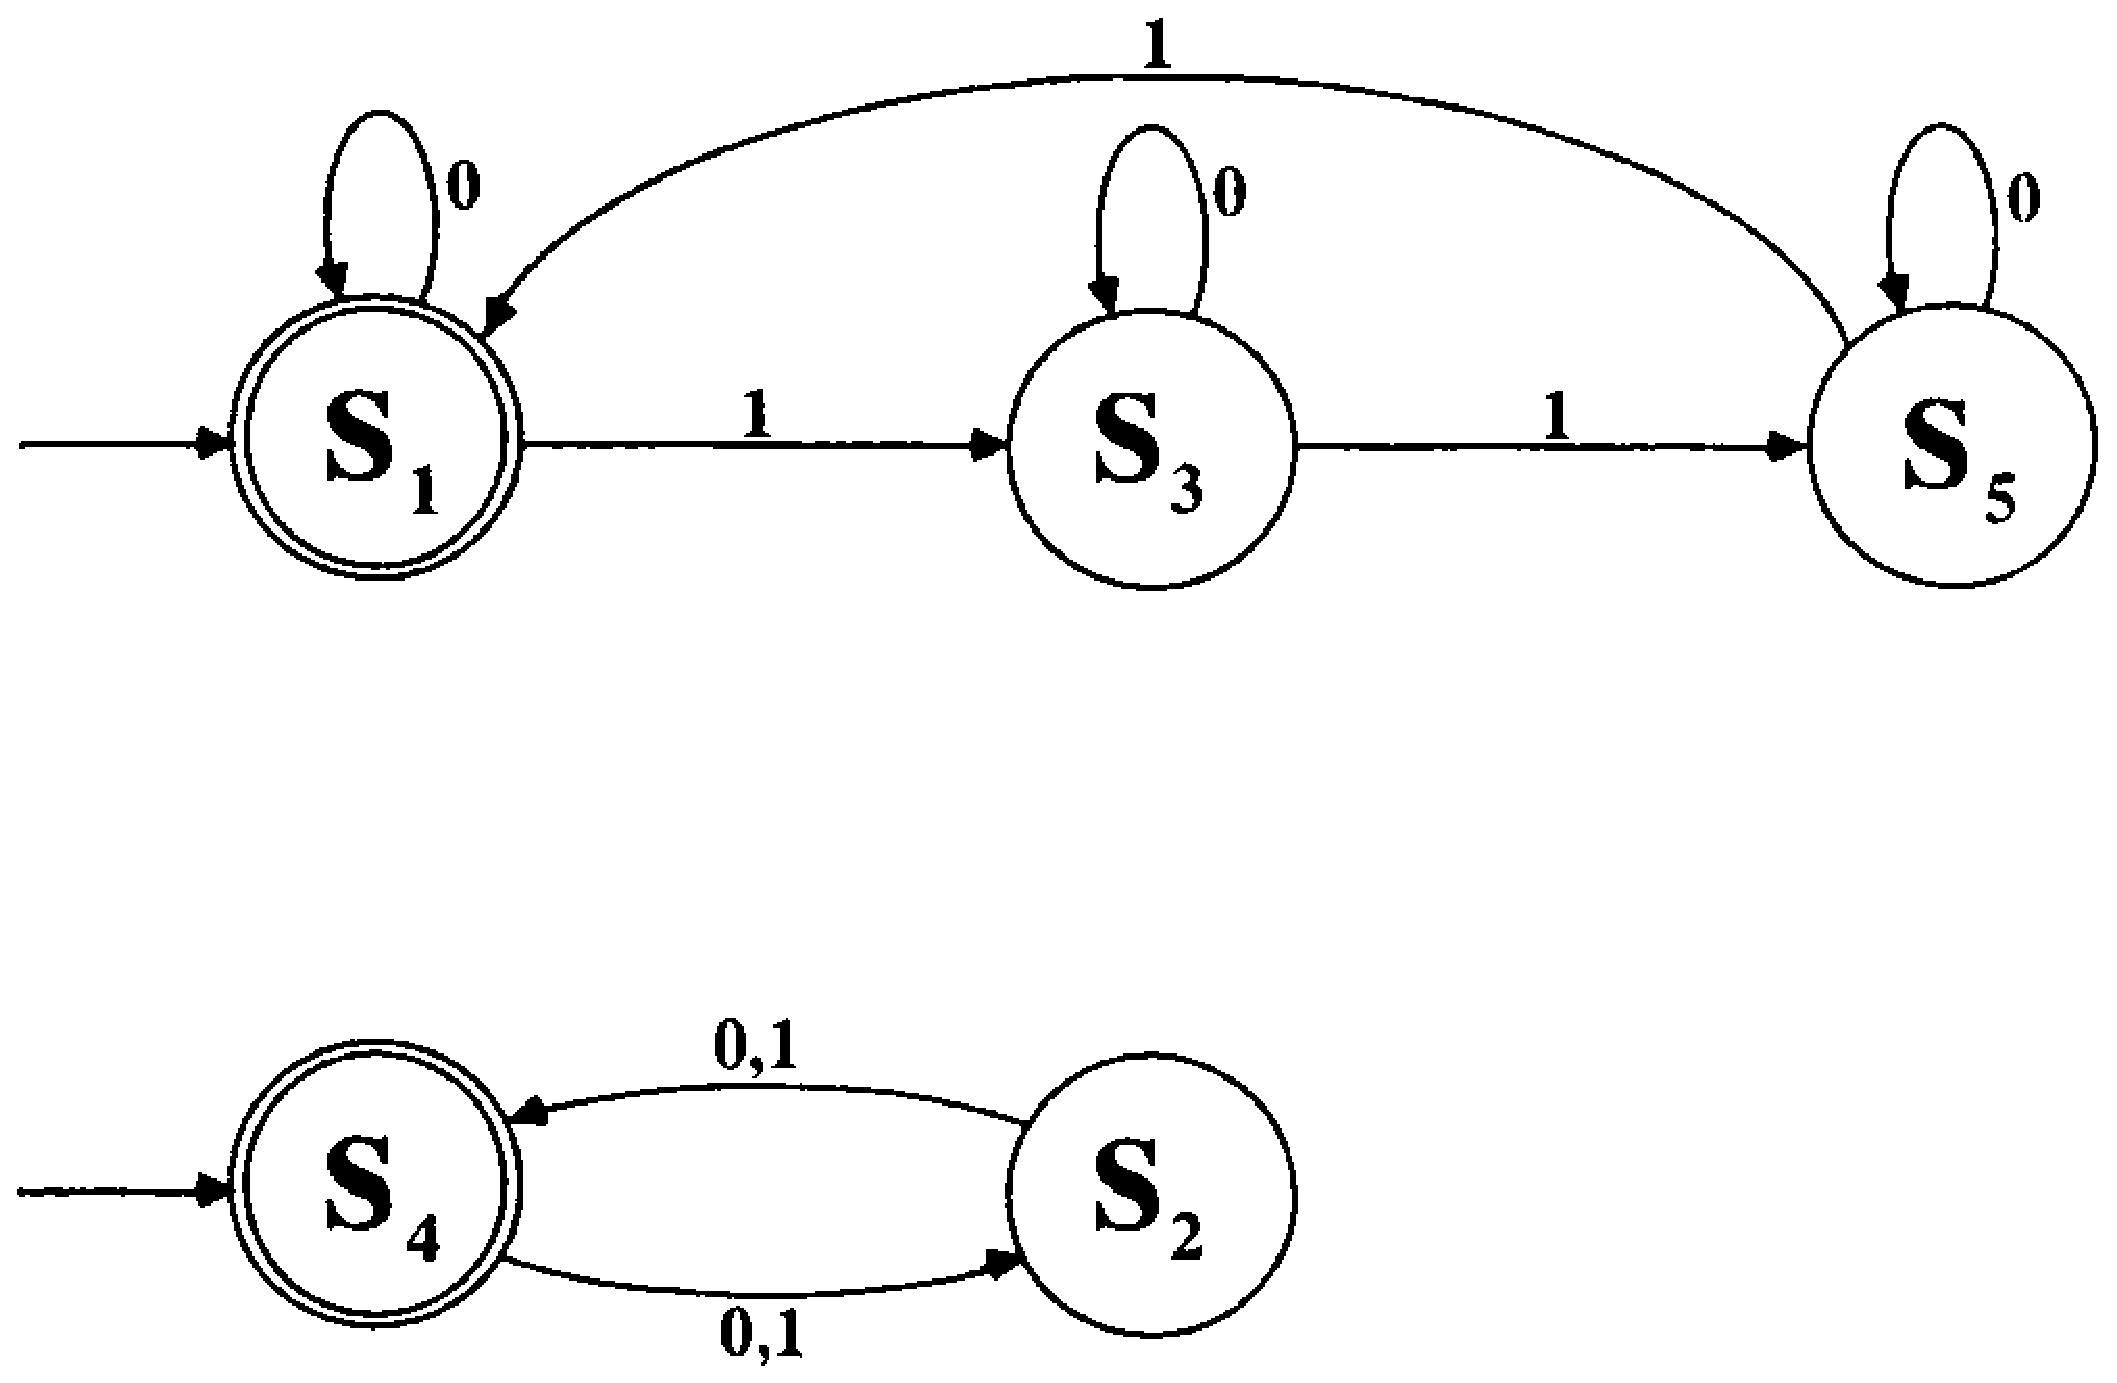
\epsfig{figure=ToFAfigures/fig4-4.eps,width=3in}}
\caption{The NDFA discussed in Example 4.3}\label{fig-4.4}
\end{figure}

As before, the addition of multiple start states to our computational model
facilitates machine construction but adds no more recognition power. We turn
now to the formal definition of nondeterministic finite automata.

% Definition 4.1
\begin{dfn}\label{dfn-4.1}\index{final state!for NDFA}\index{state transition function!for NDFA}\index{finite automaton!nondeterministic}
A \emph{nondeterministic finite automaton}\index{nondeterministic finite automaton|see{NDFA}}(\Index{NDFA}) is a
quintuple $A=\langle\Sigma,S,S_0,\delta,F\rangle$ where:
\begin{enumerate}[i.]
\item $\Sigma$ is an alphabet.\index{alphabet!input}
\item $S$ is a finite nonempty set of states.
\item $S_0$ is a \emph{set} of initial states,\index{start state} a nonempty subset of $S$.
\item $\delta:\ S \times \Sigma \rightarrow \wp(S)$ is the state transition
function.
\item $F$ is the set of accepting states, a (possibly empty) subset of $S$.
\end{enumerate}
\end{dfn}

The input alphabet, the state space, and even the set of final states are the
same as for deterministic finite automata. The important differences are
contained in the definitions of the initial states and of the $\delta$ function.

The set of initial states can be any nonempty subset of the state space. These
can be viewed as multiple entry points into the machine, with each start state
beginning distinct, although not necessarily disjoint, paths through the machine.

The $\delta$ function for nondeterministic finite automata differs from the
$\delta$ function of deterministic machines in that it maps a single state and a
letter to a set of states. In some texts, one will find $\delta$ defined as
simply a relation with range $S$ and not as a function; without any loss of
generality we define $\delta$ as a function with range $\wp(S)$, which makes
the formal proofs of relevant theorems considerably easier.

\subsection*{Example 4.4}

Consider the machine $A=\langle\Sigma,S,S_0,\delta,F\rangle$, where
\begin{center}\begin{tabular}{rcl}
$\Sigma$ & $=$ & $\{\pmb{a},\pmb{b}\}$ \\
$S$ & $=$ & $\{r,s,t\}$ \\
$S_0$ & $=$ & $\{r,s\}$ \\
$F$ & $=$ & $\{t\}$
\end{tabular}\end{center}
and $\delta:\ \{r,s,t\} \times \{\pmb{a},\pmb{b}\} \rightarrow \{\emptyset,
\{r\},\{s\},\{t\},\{s,t\},\{r,s\},\{r,t\},\{r,s,t\}\}$ is given
in Figure \ref{fig-4.5}.
% Figure 4.5
\begin{figure}[h]
\begin{center}\begin{tabular}{c|cc}
$\delta$ & $\pmb{a}$ & $\pmb{b}$ \\
\hline
r & $\{s\}$ & $\emptyset$ \\
s & $\emptyset$ & $\{r,t\}$ \\
t & $\emptyset$ & $\{t\}$
\end{tabular}\end{center}
\centerline{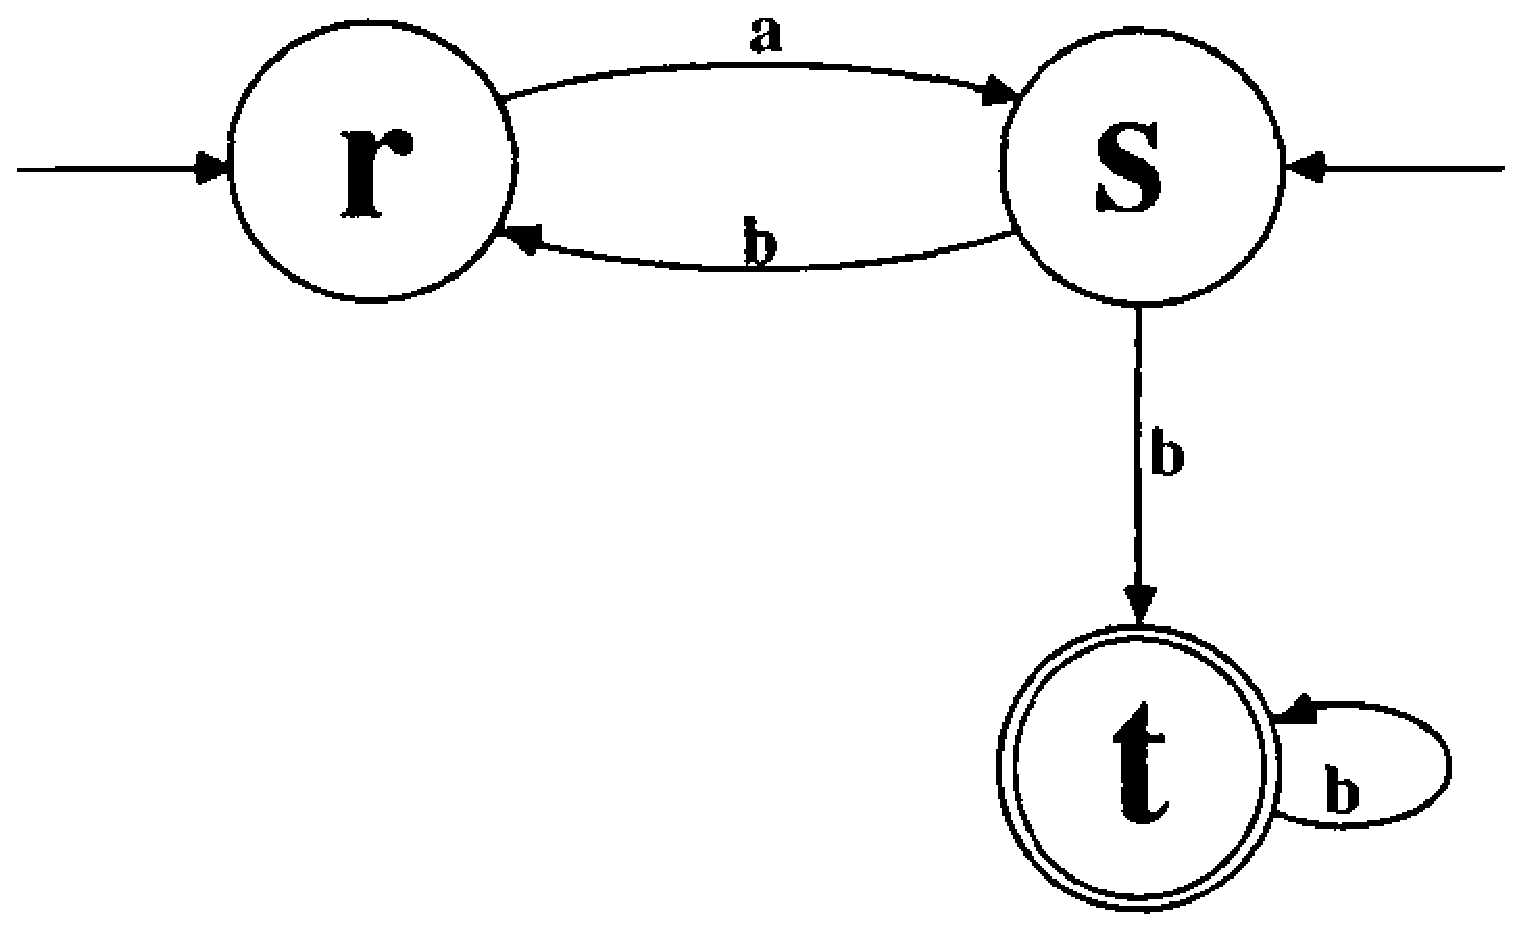
\epsfig{figure=ToFAfigures/fig4-5.eps,width=2.5in}}
\caption{An NDFA state transition diagram corresponding to the formal definition
given in Example 4.4}\label{fig-4.5}
\end{figure}

We will see later that this machine accepts strings that begin with alternating
$\pmb{a}$s and $\pmb{b}$s and end with one or more consecutive $\pmb{b}$s

% Definition 4.2
\begin{dfn}\label{dfn-4.2}\index{extended state transition function \DBAR\! for NDFA}
Given an NDFA $A=\langle\Sigma,S,S_0,\delta,F\rangle$, the
\emph{extended state transition function} for $A$ is the function $\DBAR:\ S
\times \Sigma^* \rightarrow \wp(S)$ defined recursively as follows: \\
\begin{center}\begin{tabular}{c}
$(\forall s \in S)\ \ \DBAR(s,\lambda) = \{s\}$ \\
$(\forall s \in S)(\forall\pmb{a}\in\Sigma)(\forall x \in \Sigma^*)\ \ 
	\DBAR(s,x\pmb{a}) = \bigcup\limits_{q\,\in\,\DBAR(s,x)}\delta(q,
	\pmb{a})$
\end{tabular}\end{center}
\end{dfn}

Once again, $\DBAR(s,x)$ is meant to represent where we arrive after starting at
a state $s$ and processing all the letters of the string $x$. In the case of
nondeterministic finite automata, $\DBAR$ does not map to a single state but to
a set of states because of the possible multiplicity of paths.

\subsection*{Example 4.5}

Consider again the NDFA displayed in Example 4.4. To find all the places a
string such as $\pmb{bb}$ can reach from $s$, we would first determine what can be
reached by the first $\pmb{b}$. The reachable states are $r$ and $t$, since
$\DBAR(s,\pmb{b}) = \{r, t\}$. From these states, we would then determine what
could be reached by the second $\pmb{b}$ (from $r$, no progress is possible, but
from $t$, we can again reach $t$). These calculations are reflected in the
recursive definition of $\DBAR$:
\[ \DBAR(s,\pmb{bb}) = \bigcup\limits_{q\,\in\,\DBAR(s,\pmb{b})}\delta
	(q,\pmb{b}) = \bigcup\limits_{q\,\in\,\{r,t\}}\delta(q,\pmb{b}) =
	\delta(r,\pmb{b}) \cup \delta(t,\pmb{b}) = \{\ \} \cup \{t\} = \{t\} \]

Because of the multiplicity of initial states and because the $\delta$ function
is now set-valued, it is possible for a nondeterministic finite automaton to be
active in more than a single state at one time. Whereas in all deterministic
finite automata there is a unique path through the machine labeled with
components of $w$ for each $w \in \Sigma^*$, this is not necessarily the case
for nondeterministic finite automata. At any point in the processing of a
string, the $\delta$ function maps the input symbol and the current state to a
set of states. This implies that multiple paths through the machine are possible
or that the machine can get ``stuck'' and be unable to process the remainder of
the string if there is no transition from a state labeled with the appropriate
letter. There is no more than one path for each word if there is exactly one
start state and the $\delta$ function always maps to a singleton set (or
$\emptyset$). If we were to further require that the $\delta$ function have a
defined transition to another state for every input symbol, then the machine
that we have would essentially be a deterministic finite automaton. Thus, all
deterministic finite automata are simply a special class of nondeterministic
finite automata; with some trivial changes in notation, any DFA can be thought
of as an NDFA. Indeed, the state transition diagram of a DFA could be a picture
of a well-behaved NDFA. Therefore, any language accepted by a DFA can be
accepted by an NDFA.

\subsection*{Example 4.6}

Consider the machine given in Example 4.4 and let $x = \pmb{b}$; the possible
paths through the machine include (1) starting at $s$ and proceeding to $r$, and
(2) starting at $s$ and proceeding to $t$. Note that it is not possible to start
from $t$ (since $t \notin S_0$), and there is no way to proceed with $x =
\pmb{b}$ by starting at $r$, the other start state.

Now let $x = \pmb{ba}$ and consider the possibilities. The only path through the
machine requires that we start at $s$, proceed to $r$, and return to $s$;
starting at $s$ and proceeding to $t$ leaves no way to process the second letter
of $x$. Starting from $r$ is again hopeless (what types of strings are good
candidates for starting at $r$?).

Now let $x = \pmb{bab}$; the possible paths through the machine include (1)
starting at $s$, proceeding to $r$, returning to $s$, and then moving again to
$r$, and (2) starting at $s$, proceeding to $r$, returning to $s$, and then
proceeding to $t$. Note that starting at $s$ and moving immediately to $t$ again
leaves us with no way to process the remainder of the string. Both $\pmb{b}$ and
$\pmb{bab}$ included paths that terminated at the final state $t$ (among other
places). These strings will be said to be \emph{recognized} by this NDFA
(compare with Definition \ref{dfn-4.3}). $\pmb{ba}$ had no path that led to a final state,
and as a consequence we will consider $\pmb{ba}$ to be rejected by this machine.

There are a number of ways in which to conceptualize a nondeterministic
finite automaton. Among the most useful are the following two schemes:

\begin{enumerate}
\item At each state where a multiple transition occurs, the machine replicates
into identical copies of itself, with each copy following one of the possible
paths.
\item Multiple states of the machine are allowed to be active, and each of the
active states reacts to each input letter.
\end{enumerate}

It happens that the second viewpoint is the most useful for our purposes. From
a theoretical point of view, we use this as the basis for proving the
equivalence of deterministic and nondeterministic finite automata. It is also a
useful model upon which to base the circuits that implement NDFAs.

The concept of a language for nondeterministic finite automata is different
from that for deterministic machines. Recall that the requirement for a word
to be contained in the language accepted by a deterministic finite automaton was
that the processing of a string would terminate in a final state. This is also
the condition for belonging to the \emph{language} accepted by a
nondeterministic finite automaton; however, since the path through a
nondeterministic finite automaton is not necessarily unique, only one of the
many possible paths need terminate in a final state for the string to be
accepted.

% Definition 4.3
\begin{dfn}\label{dfn-4.3}
Let $A=\langle\Sigma,S,S_0,\delta,F\rangle$ be a nondeterministic finite
automaton and $w$ be a word in $\Sigma^*$. A accepts $w$ iff 
$(\bigcup\limits_{q\,\in S_0}\DBAR(q,w)) \cap F \not= \emptyset$.
\end{dfn}

Again conforming with our previous usage, a word that is not accepted is
\emph{rejected}. The use of the operator $L$ will be consistent with its usage in
previous chapters, although it does have a different formal definition. As
before, $L(A)$ is used to designate all those strings that are accepted by a
finite automaton $A$. Since the concept of \emph{acceptance} must be modified
for nondeterministic finite automata, the formal definition of $L$ is
necessarily different (contrast Definitions \ref{dfn-4.3} and \ref{dfn-1.12}).

% Definition 4.4
\begin{dfn}\label{dfn-4.4}
Given an NDFA $A=\langle\Sigma,S,S_0,\delta,F\rangle$, the language accepted
by $A$, denoted $L(A)$, is given by
\[L(A) = \{x \in \Sigma^*\,\,|\,\,(\bigcup\limits_{q\,\in S_0}
\DBAR(q,x)) \cap F \not= \emptyset\}\]
\end{dfn}

Occasionally, it will be more convenient to express $L(A)$ in the following
fashion: $L(A) = \{x \in \Sigma^*|\exists t \in S_0 \ni \DBAR(t,x) \cap F \not=
\emptyset\}$. The concept of \emph{equivalent} automata is unchanged: two
machines are equivalent \emph{iff} they accept the same language. Thus, if one
or both of the machines happen to be nondeterministic, the definition still
applies. For example, the NDFAs given in Figures \ref{fig-4.3} and \ref{fig-4.4} are equivalent.

The language recognized by a nondeterministic finite automaton is the set of
all words where at least one of the paths through the machine labeled with
components of that word ends in a final state. In other words, the set of
terminal states at the ends of the paths labeled by components of a word $w$
must have a state in common with the set of final states in order for $w$ to
belong to $L(A)$.

As a first example, refer to the NDFA defined in Example 4.4. As illustrated
in Example 4.6, this machine accepts strings that begin with alternating
$\pmb{a}$s and $\pmb{b}$s and end with one or more consecutive $\pmb{b}$s.

\subsection*{Example 4.7}

For a more concrete example, consider the problem of a ship attempting to
transmit data to shore at random intervals. The receiver must continually
listen, usually to noise, and recognize when an actual transmission starts so
that it can record the data that follow. Let us assume that the start of a
transmission is signaled by the string $\pmb{010010}$ (in practice, such a
signal string should be much longer to minimize the possibility of random noise
triggering the recording mechanism). In essence, we wish to build an NDFA that
will monitor a bit stream and move to a final state when the substring
$\pmb{010010}$ is detected (note that nonfinal states correspond to having the
recording mechanism off, and final states signify that the current data should
be recorded). The reader is encouraged to discover firsthand how hard it is to
build a DFA that correctly implements this machine and contrast that solution to
the NDFA $T$ given in Figure \ref{fig-4.6}.

% Figure 4.6
\begin{figure}
\centerline{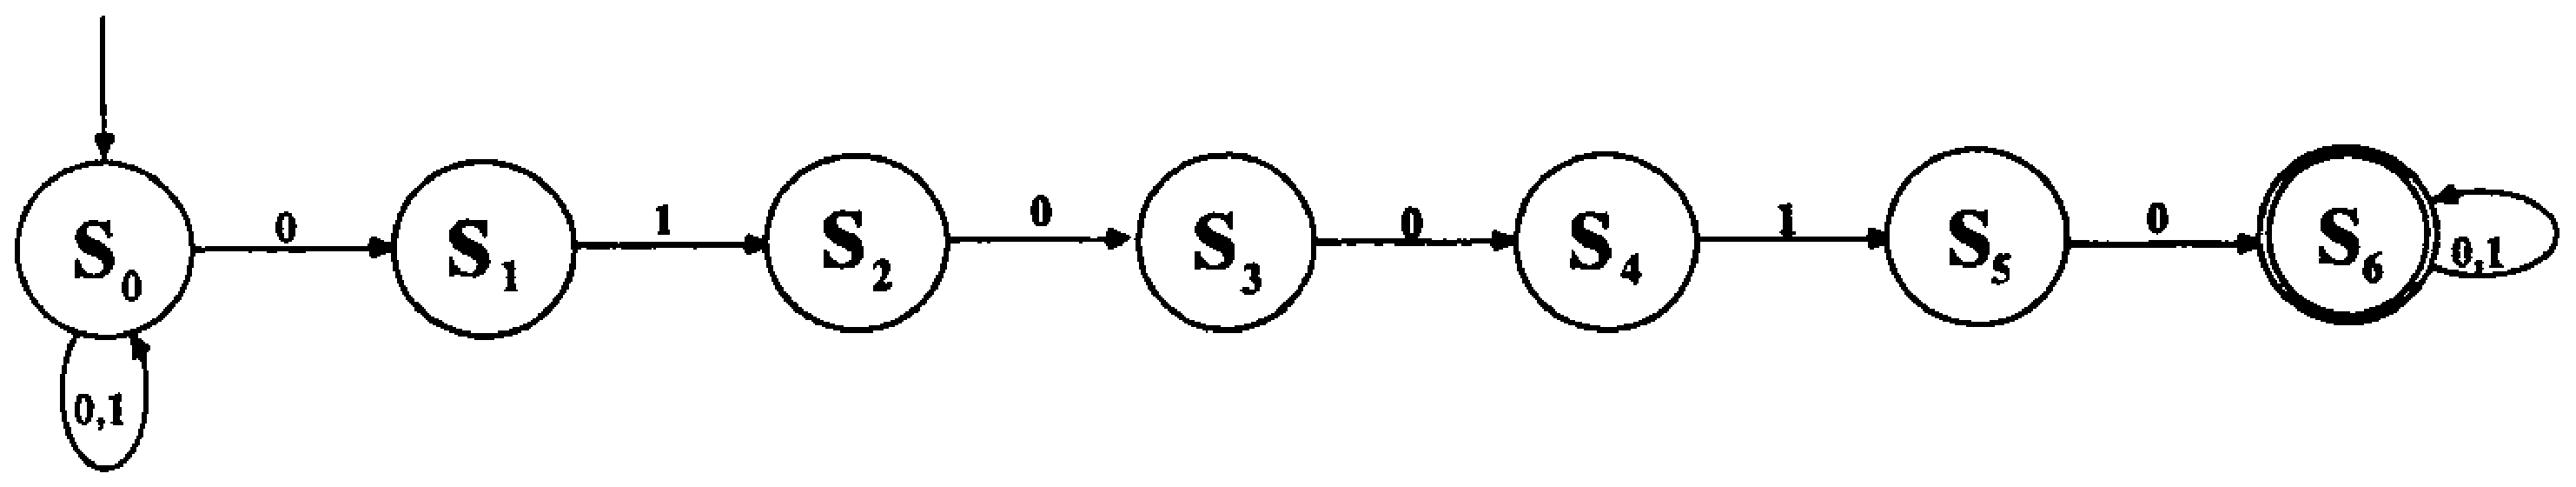
\epsfig{figure=ToFAfigures/fig4-6.eps,width=6.5in}}
\caption{An NDFA for pattern recognition}\label{fig-4.6}
\end{figure}

Since the transitions leading to higher states are labeled by the symbols in
$\pmb{010010}$, it is clear that the last state cannot be reached unless the
sequence $\pmb{010010}$ is actually scanned at some point during the processing
of the input string. Thus, the NDFA clearly accepts no word that should be
rejected. Conversely, since \emph{all} possible legal paths are explored by an
NDFA, valid strings \emph{will} find a way to the final state. lt is sometimes
helpful to think of the NDFA as remaining in $s_0$ while the initial part of the
input string is being processed and then ``guessing'' when it is the right time
to move to $s_1$.

It is also possible to model an end-of-transmission signal that turns the
recording device off (see the exercises). The device would remain in various
final states until a valid end-of-transmission string was scanned, at which
point it would return to the (nonfinal) start state.

While the NDFA given in Example 4.6 is very straightforward, it appears to be
hard to simulate this nondeterminism in real time with a deterministic computer.
It has not been difficult to keep track of the multiple paths in the simple
machines seen so far. However, if each state has multiple transitions for a
given symbol, the number of distinct paths a single word can take through an
NDFA grows exponentially as the length of the word increases. For example, if
each transition allowed a choice of three destination states, a word of length
$m$ would have $3^m$ possible paths from one single start state. An improvement
can be made by calculating, as each letter is processed, the set of possible
\emph{destinations} (rather than recording all the \emph{paths}). Still, in an
$n$-state NDFA, there are potentially $2^n$ such combinations of states. This
represents an improvement over the path set, since now the number of state
combinations is independent of the length of the particular word being
processed; it depends only on the number of states in the NDFA, which is
fixed. We will see that keeping track of the set of possible destination states
is indeed the best way to handle an NDFA in a deterministic manner.

Since we have seen in Chapter \ref{ch-1} that it is easy to implement a DFA, we now
explore methods to convert an NDFA to an equivalent DFA. Suppose that we are
given a nondeterministic finite automaton $A$ and that we want to construct a
corresponding deterministic finite automaton $A^d$. Using the concepts in
Definitions \ref{dfn-4.1} through \ref{dfn-4.4}, we can proceed in the following fashion. Our
general strategy will be to keep track of all the states that can be reached by
some string in the nondeterministic finite automaton. Since we can arbitrarily
label the states of an automaton, we let the state space of $A^d$ be the
\emph{power set} of $S$. Thus, $S^d = \wp(S)$, and each state in the new
machine will be labeled by some subset of $S$. Furthermore, let the start state
of $A^d$, denoted $s^d_0$, be labeled by the member of $\wp(S)$ containing
those states that are initial states in $A$; that is, $s^d_0 = S_0$.

Since our general strategy is to ``remember'' all the states that can be reached
for some string, we can define the $\delta$ function in the following natural
manner: For every letter in $\Sigma$, let the new state transition function,
$\delta^d$, map to the subset of $\wp(S)$ labeled by the union of all those
states that are reached from some state contained in the current state name
(according to the old nondeterministic state transition function $\delta$).

According to Definition \ref{dfn-4.4}, for a word to be contained in the language accepted
by some nondeterministic finite automaton, at least one of the terminal states
was required to be contained in the set of final states. Thus, let the set of
final states in the corresponding deterministic finite automaton be labeled by
the subsets of $S$ that contain at least one of the accepting states in the
nondeterministic counterpart. The formal definition of our corresponding
deterministic finite automaton is given in Definition \ref{dfn-4.5}.

% Definition 4.5
\begin{dfn}\label{dfn-4.5}
Given an NDFA $A=\langle\Sigma,S,S_0,\delta,F\rangle$, the
\emph{\Index{corresponding deterministic finite automaton}}, $A^d=\langle\Sigma,
S^d,s^d_0,\delta^d,F^d\rangle$, is defined as follows:
\begin{center}\begin{tabular}{c}
$S^d = \wp(S)$ \\
$s^d_0 = S_0$ \\
$F^d = \{Q \in S^d|Q \cap F \not= \emptyset\}$
\end{tabular}\end{center}
and $\delta^d$ is the state transition function, $\delta^d$$:\ S^d \times \Sigma
\rightarrow S^d$, defined by
\[ (\forall Q \in S^d)(\forall\pmb{a}\in\Sigma)\delta^d(Q,\pmb{a}) =
	\bigcup\limits_{q\,\in\, Q} \delta(q,\pmb{a}) \]
$\delta^d$ extends to the function $\deltabar{d}\!\!:\ S^d \times \Sigma^* \rightarrow
S^d$ as suggested by Theorem \ref{thm-1.1}:
\begin{center}\begin{tabular}{l}
$(\forall Q \in S^d)\qquad\qquad\qquad\qquad\ \deltabar{d}(Q,\lambda) = Q$ \\
$(\forall Q \in S^d)(\forall\pmb{a}\in\Sigma)(\forall x \in
	\Sigma^*)\deltabar{d}(Q,x\pmb{a}) = \delta^d(\deltabar{d}(Q,x),\pmb{a})$
\end{tabular}\end{center}
\end{dfn}

Definition \ref{dfn-4.5} describes a deterministic finite automaton that observes the
same restrictions as all other deterministic finite automata (a single start
state, a finite state set, a well-defined transition function, and so on). The
only peculiarity is the labeling of the states. Note that the definition implies
that the state labeled by the empty set is \emph{never} a final state and that
all transitions from this state lead back to itself. This is the dead state,
which is reached by strings that are always prematurely terminated in the
corresponding nondeterministic machine.

\subsection*{Example 4.8}

Consider the NDFA $B$ given in Figure \ref{fig-4.7}. As specified by Definition \ref{dfn-4.5}, the
corresponding DFA $B^d$ would look like the machine shown in Figure \ref{fig-4.8}. Note
that all the states happen to be accessible in this particular example.

% Figure 4.7
\begin{figure}
\centerline{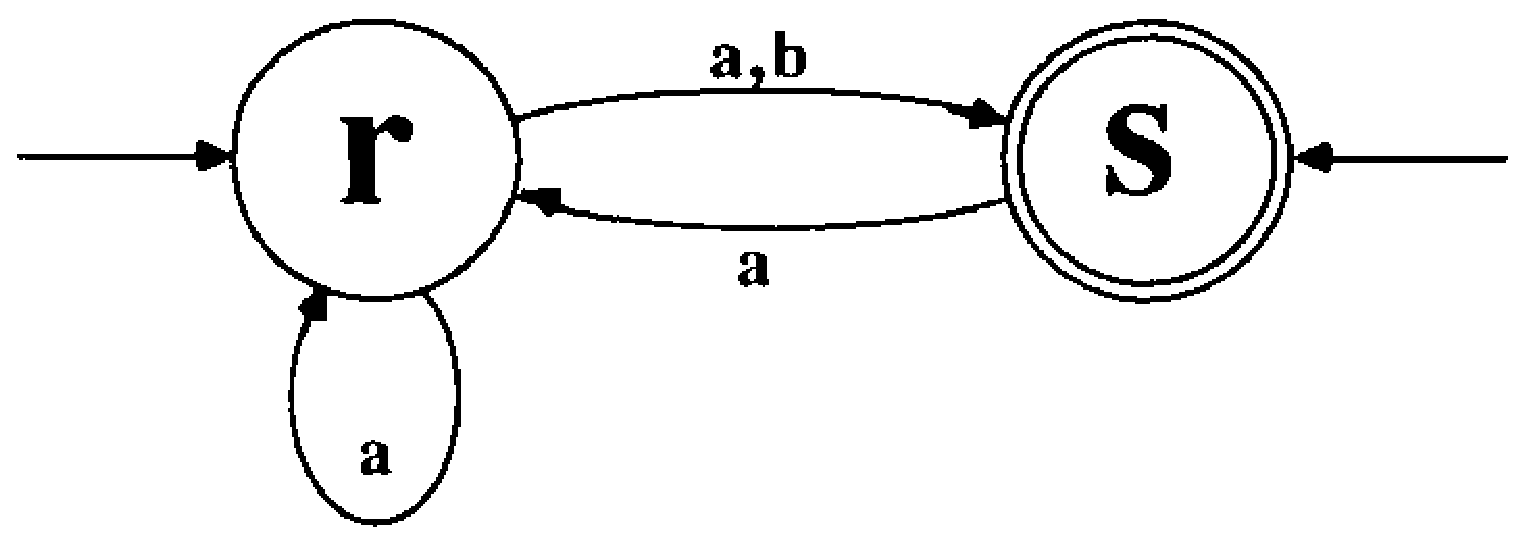
\epsfig{figure=ToFAfigures/fig4-7.eps,width=2.8in}}
\caption{The NDFA B discussed in Example 4.8}\label{fig-4.7}
\end{figure}

Since the construction of the corresponding deterministic machine involves
$\wp(S)$, it should be obvious to the reader that the size of this
deterministic finite automaton \emph{can} grow exponentially larger as the number of
states in the associated nondeterministic finite automaton increases. In
general, however, there are often many inaccessible states. Thus, only the
states that are found to be reachable during the construction process need to be
included. The reader is encouraged to exploit this fact when constructing
corresponding deterministic finite automata. The language accepted by the DFA
$A^d$ follows the definition given in Chapter \ref{ch-1}.

% Figure 4.8
\begin{figure}
\centerline{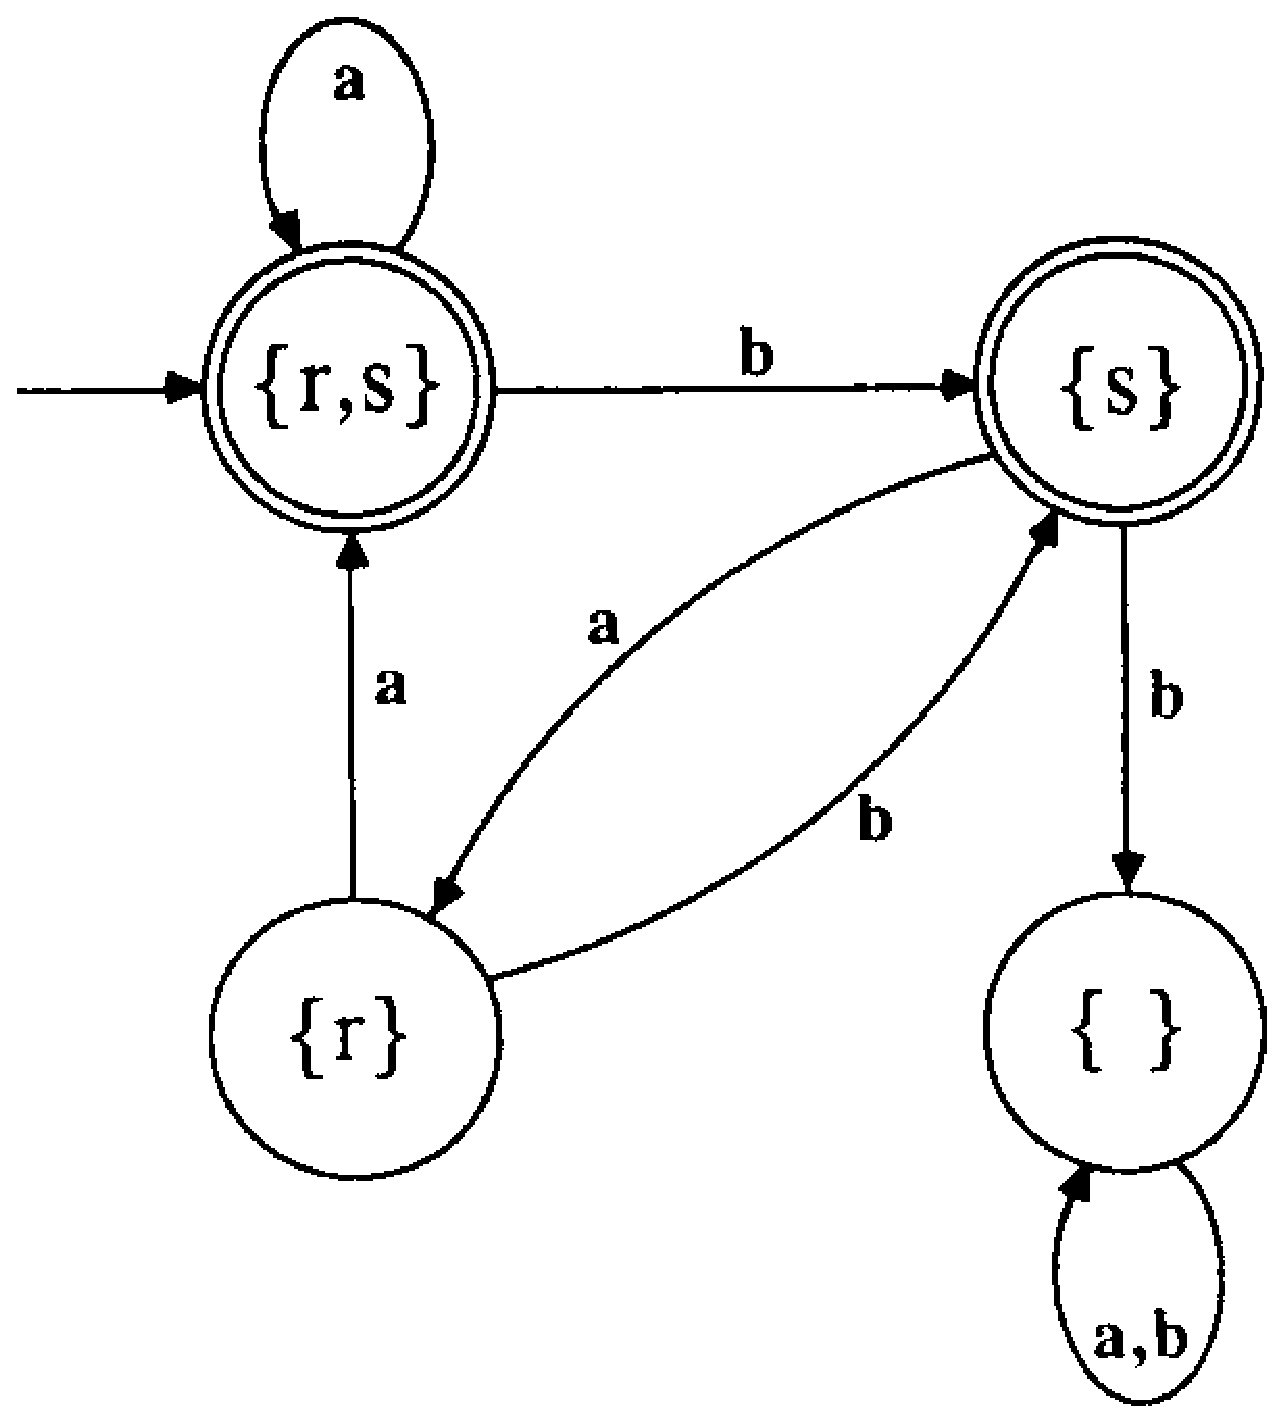
\epsfig{figure=ToFAfigures/fig4-8.eps,width=2.5in}}
\caption{The deterministic equivalent of the NDFA given in Example 4.8}\label{fig-4.8}
\end{figure}

To show that the deterministic finite automaton that we have just defined
accepts the same language as the corresponding nondeterministic finite
automaton, we must first show that the $\deltabar{d}$ function behaves in the same
manner for strings as the $\delta^d$ function does for single letters. For any
state $Q \in S^d$, the $\delta^d$ function maps this state and an input letter
$\pmb{a} \in \Sigma$ according to the mapping of the $\delta$ function for each
$q \in Q$ and the letter $\pmb{a}$. The following lemma establishes that $\deltabar{d}$
performs the corresponding mapping for strings.

% Lemma 4.1
\begin{lmm}\label{lmm-4.1}
Let $A=\langle\Sigma,S,S_0,\delta,F\rangle$ be a nondeterministic finite
automaton, and let $A^d=\langle\Sigma,S^d,s^d_0,\delta^d,F^d\rangle$ represent
the corresponding deterministic finite automaton. Then
\[ (\forall Q \in S^d)(\forall x \in \Sigma^*)(\deltabar{d}(Q,x) =
	\bigcup\limits_{q\,\in\, Q} \DBAR(q,x)) \]

\emph{Proof.} By induction on $|x|$: Let $P(k)$ be defined by
\[ P(k):\ (\forall Q \in S^d)(\forall x \in \Sigma^k)(\deltabar{d}(Q,x) =
	\bigcup\limits_{q\,\in\, Q} \DBAR(q,x)) \]
\emph{Basis step:} $|x| = 0 \Rightarrow x = \lambda$ and therefore
\[ \deltabar{d}(Q,\lambda) = Q = \bigcup\limits_{q\,\in\, Q}\{q\} = 
	\bigcup\limits_{q\,\in\, Q}\DBAR(q,\lambda) \]
\emph{Inductive step:} Suppose that the result holds for all $x \ni |x| = k$;
that is, $P(k)$ is true. Let $y \in \Sigma^{k+1}$. Then $\exists x \in \Sigma^k$
and $\exists \pmb{a} \in \Sigma \ni y = x\pmb{a}$. Then
\begin{center}\begin{tabular}{rcl}
$\deltabar{d}(Q,y)$ & $=$ & (by definition of $y$) \\
$\deltabar{d}(Q,x\pmb{a})$ & $=$ & (by Theorem \ref{thm-1.1}) \\
$\delta^d(\deltabar{d}(Q,x),\pmb{a})$ & $=$ & (by the induction hypothesis) \\
$\delta^d(\bigcup\limits_{q\,\in\, Q}\DBAR(q,x),\pmb{a})$ & $=$ & $(\forall A,B
	\in \wp(S))(\forall\pmb{a}\in\Sigma)(\delta^d(A \cup B,\pmb{a}) =
	\delta^d(A,\pmb{a}) \cup \delta^d(B,\pmb{a}))$ \\
$\bigcup\limits_{q\,\in\, Q}\delta^d(\DBAR(q,x),\pmb{a})$ & $=$ &
	(by Definition \ref{dfn-4.5}) \\
$\bigcup\limits_{q\,\in\, Q}(\bigcup\limits_{p\,\in\,\DBAR(q,x)}\delta
	(p,\pmb{a}))$ & $=$ & (by Definition \ref{dfn-4.2}) \\
$\bigcup\limits_{q\,\in\, Q}\DBAR(q,x\pmb{a})$ & $=$ & (by definition of $y$) \\
$\bigcup\limits_{q\,\in\, Q} \DBAR(q,y)$ &&
\end{tabular}\end{center}
Therefore, $P(k) \Rightarrow P(k+1)$ for all $k \geq 0$, and thus by the
principle of mathematical induction we can say that the result holds for all
$x \in \Sigma^*$.
\end{lmm}

Having established Lemma \ref{lmm-4.1}, proving that the language accepted by a
nondeterministic finite automaton and the corresponding deterministic machine
are the same language becomes a straightforward task. The equivalence of $A$ and
$A^d$ is given in the following theorem.

% Theorem 4.1
\begin{thm}\label{thm-4.1}
Let $A=\langle\Sigma,S,S_0,\delta,F\rangle$ be a nondeterministic finite
automaton, and let $A^d=\langle\Sigma,S^d,s^d_0,\delta^d,F^d\rangle$ represent
its corresponding deterministic finite automaton. Then $A$ and $A^d$ are
equivalent; that is, $L(A) = L(A^d)$.

\emph{Proof.} Let $x \in \Sigma^*$. Then
\begin{center}\begin{tabular}{rcl}
$x \in L(A)$ & $\Leftrightarrow$ & (by Definition \ref{dfn-4.4}) \\
$(\bigcup\limits_{s \in S_0}\DBAR(s,x)) \cap F \not= \emptyset$ &
	$\Leftrightarrow$ & (by Definition \ref{dfn-4.5}) \\
$(\bigcup\limits_{s\,\in\, S_0}\DBAR(s,x)) \in F^d$ & $\Leftrightarrow$ &
	(by Lemma \ref{lmm-4.1}) \\
$\DBAR^d(S_0,x) \in F^d$ & $\Leftrightarrow$ & (by Definition \ref{dfn-4.5}) \\
$\DBAR^d(s^d_0,x) \in F^d$ & $\Leftrightarrow$ & (by Definition \ref{dfn-1.15}) \\
$x \in L(A^d)$ &&
\end{tabular}\end{center}
\end{thm}

Now that we have established that nondeterministic finite automata and
deterministic finite automata are equal in computing power, the reader might
wonder why we bother with nondeterministic finite automata. Even though
nondeterministic finite automata cannot recognize any language that cannot be
defined by a DFA, they are very useful both in theory and in machine
construction (as illustrated by Example 4.7). The following examples further
illustrate that NDFAs often yield more natural (and less complex) solutions to a
given problem.

\subsection*{Example 4.9}

Recall the machine from Chapter \ref{ch-1} that accepted a subset of real constants in
scientific notation according to the following BNF:\index{BNF}\index{natural numbers}
\begin{center}
\begin{center}\begin{tabular}{rcl}
\hline
\<sign\> & ::= & $ \pmb + | \pmb -$ \\
\<digit\> & ::= & $ \pmb 0|\pmb 1|\pmb 2|\pmb 3|\pmb 4|\pmb 5|\pmb 6|\pmb 7|\pmb 8|\pmb 9$ \\
\<natural\> & ::= & \<\text{digit}\>$|$\<digit\>\<natural\> \\
\<integer\> & ::= & \<natural\>$|$\<sign\>\<natural\> \\
\<real constant\> & ::= & \<integer\> \ \ \ \ \ \ \ \ \ \ \ \ \ \ \ \ \ \ \ \ \ \ \ \ $|$ \\
 & &\ \ \<integer\>\pmb{.}  \ \ \ \ \ \ \ \ \ \ \ \ \ \ \ \ \ \ \ \ \ $|$ \\
 & &\ \ \<integer\>\pmb{.}\<natural\> \ \,$|$ \\
 & &\ \ \<integer\>\pmb{.}\<natural\>\pmb{E}\<integer\> \\
\hline
\end{tabular}\end{center}
\end{center}
By using nondeterministic finite automata, it is easy to construct a machine
that will recognize this language (compare with the deterministic version given
in Example 1.11). One such NDFA is shown in Figure \ref{fig-4.9}.


% Figure 4.9
\begin{figure}
\centerline{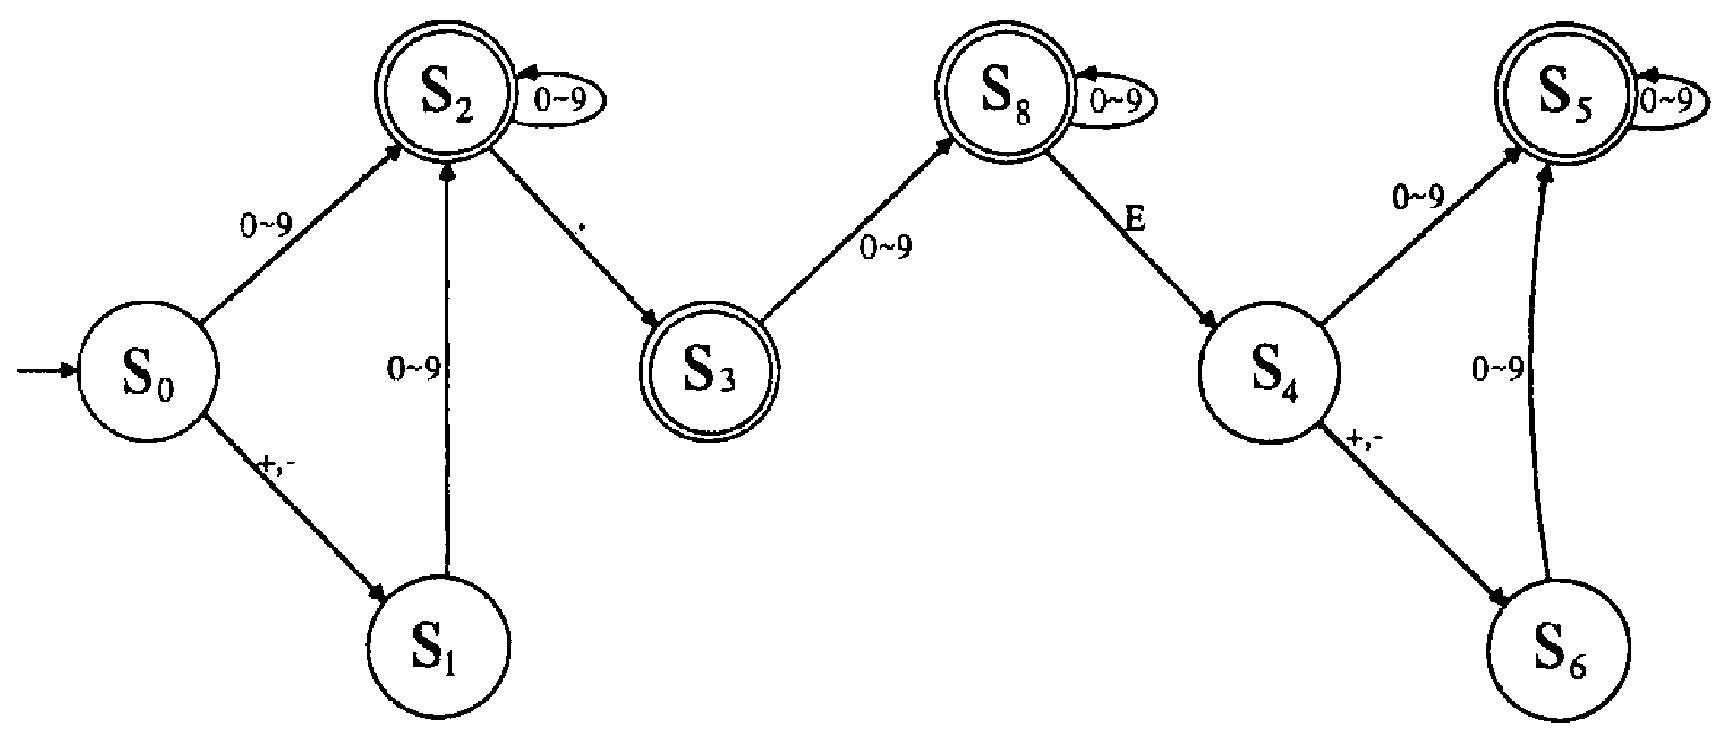
\epsfig{figure=ToFAfigures/fig4-9.eps,width=6in}}
\caption{The NDFA discussed in Example 4.9}\label{fig-4.9}
\end{figure}

\subsection*{Example 4.10}

Let $L=\{x \in \{\pmb{a},\pmb{b}\}^*|\ x$ begins with $\pmb{a}\vee x$ contains
$\pmb{ba}$ as a substring$\}$. We can easily build a machine that will accept
this language, as illustrated in Figure \ref{fig-4.10}. Now suppose we wanted to construct
a machine that would accept the \emph{reverse} of this language, that is, to accept
$L^r=\{x \in \{\pmb{a},\pmb{b}\}^*|\ x$ ends with $\pmb{a}\vee x$ contains
$\pmb{ab}\}$. The machine that will accept this language can be built using
nondeterministic finite automata by simply exchanging the initial states and the
final states and by reversing the arrows of the $\delta$ function. The automaton
(definitely an NDFA in this case!) arising in this fashion is shown in Figure
\ref{fig-4.11}.

% Figure 4.10
\begin{figure}
\centerline{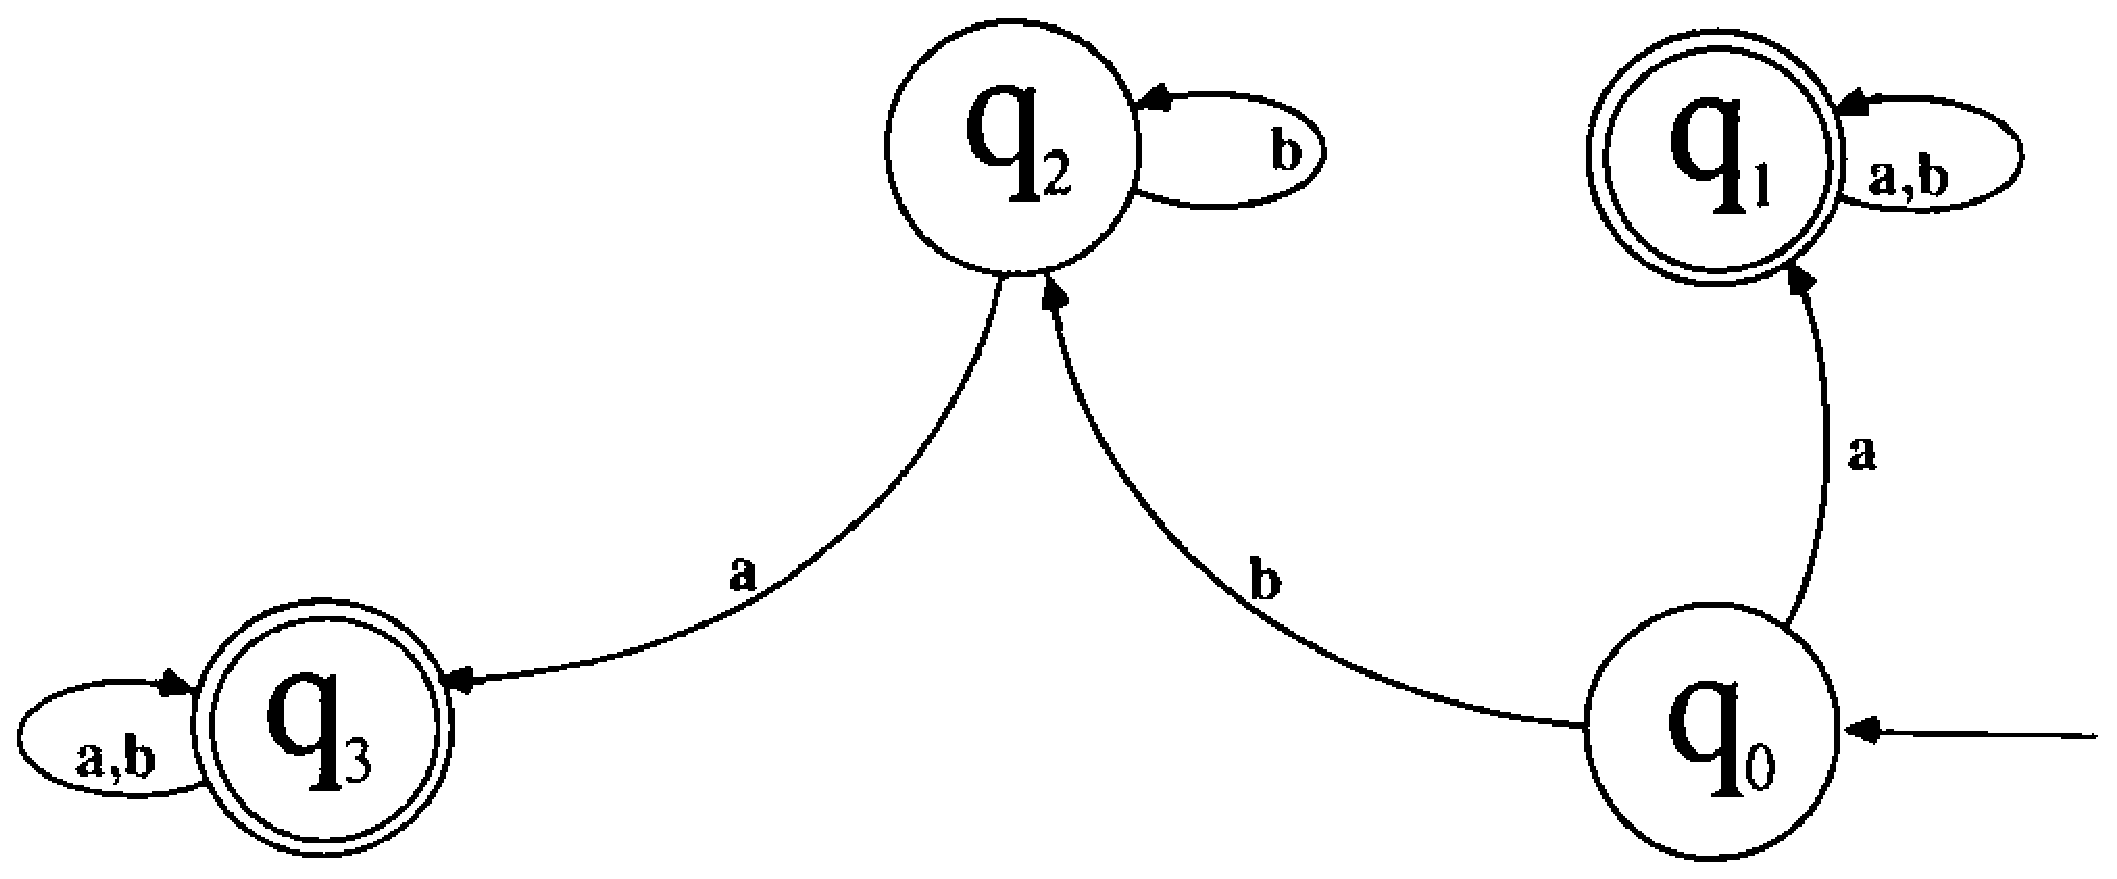
\epsfig{figure=ToFAfigures/fig4-10.eps,width=3.5in}}
\caption{An NDFA accepting the language given in Example 4.10}\label{fig-4.10}
\end{figure}

It can be shown that the technique employed in Example 4.10, when applied to \emph{any}
automaton, will yield a new NDFA that is guaranteed to accept the \emph{reverse}
of the original language. The material in Chapter \ref{ch-5} will reveal many instances
where the ability to define multiple start states and multiple transitions will
be of great value.

% Figure 4.11
\begin{figure}
\centerline{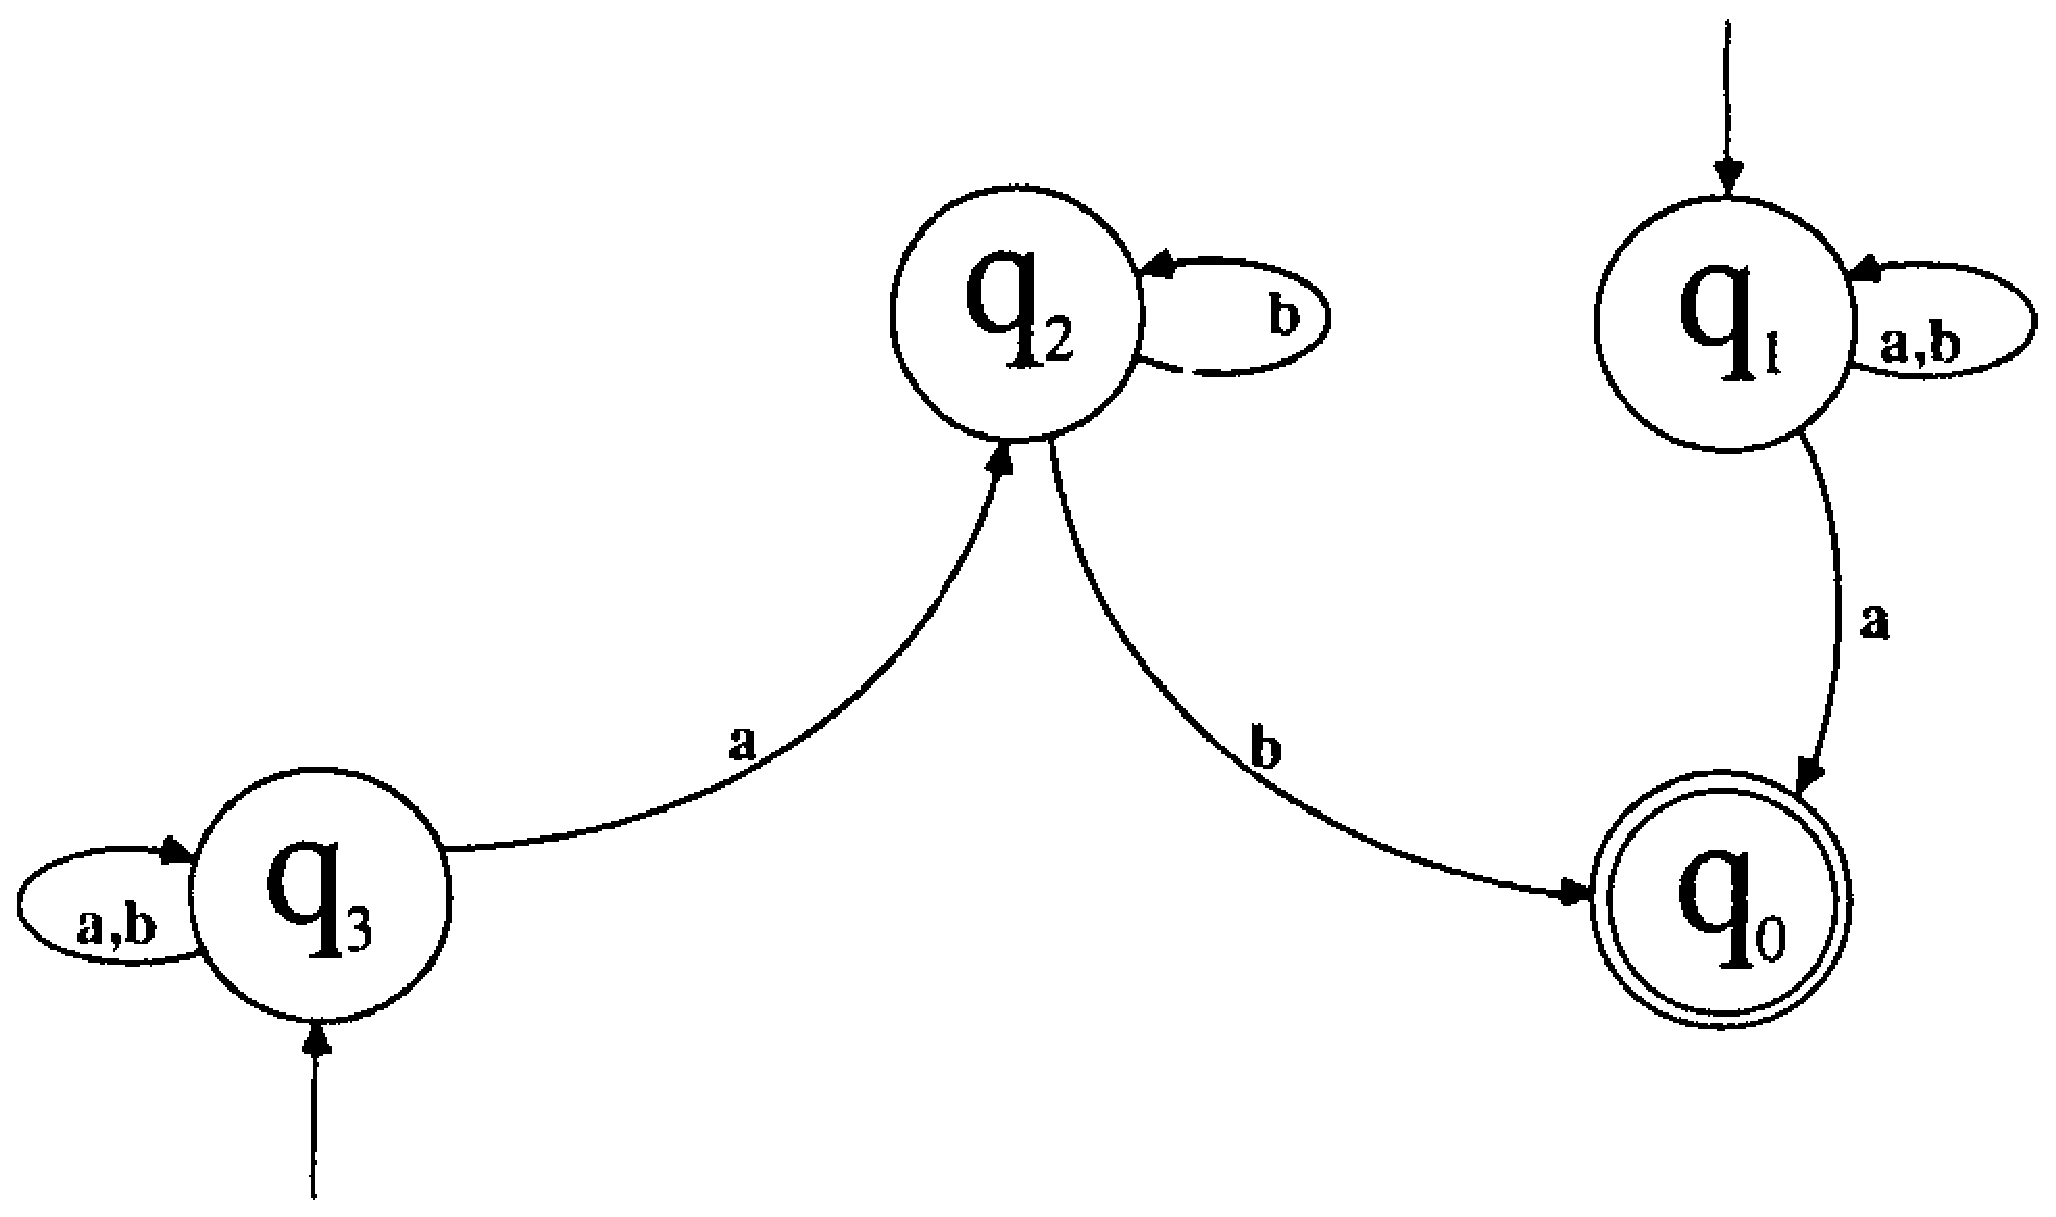
\epsfig{figure=ToFAfigures/fig4-11.eps,width=3.5in}}
\caption{An NDFA representing the reverse of the language represented in
Figure \ref{fig-4.10}}\label{fig-4.11}
\end{figure}

\subsection*{Example 4.11}

Assume we wish to identify all words that contain at least one of the three
strings $\pmb{10110},\ \pmb{1010}$, or $\pmb{01101}$ as substrings. Consequently, we let L be the set of all
words that are made up of some characters, followed by one of our three target
strings, followed by some other characters. That is,
\[ L=\{w \in \{\pmb{0},\pmb{1}\}^*|\ w=xyz,x \in \{\pmb{0},\pmb{1}\}^*,y \in
	\{\pmb{10110},\pmb{1010},\pmb{01101}\},z \in \{\pmb{0},\pmb{1}\}^*\} \]
We can construct a nondeterministic finite automaton that will accept this
language as follows. First construct three machines each of which will accept
one of the candidates for $y$. Next, prepend a single state ($s_0$ in Figure
\ref{fig-4.12}) that loops on $\Sigma^*$; make this state an initial state and draw arrows
from it which mimic the transitions from each of the other three initial states
(as shown in Figure \ref{fig-4.12}). Finally, append a single state machine ($S_{18}$)
that accepts $\Sigma^*$; draw arrows from each of the final states to this state. The machine that accepts this language is given in Figure \ref{fig-4.12}.
The reader is encouraged to try to construct a deterministic version of this
machine in order to appreciate the simplicity of the above solution.
(States $s_1$, $s_7$, and $s_{12}$ are shown for clarity,
but they are no longer needed.)

% Figure 4.12
\begin{figure}
\centerline{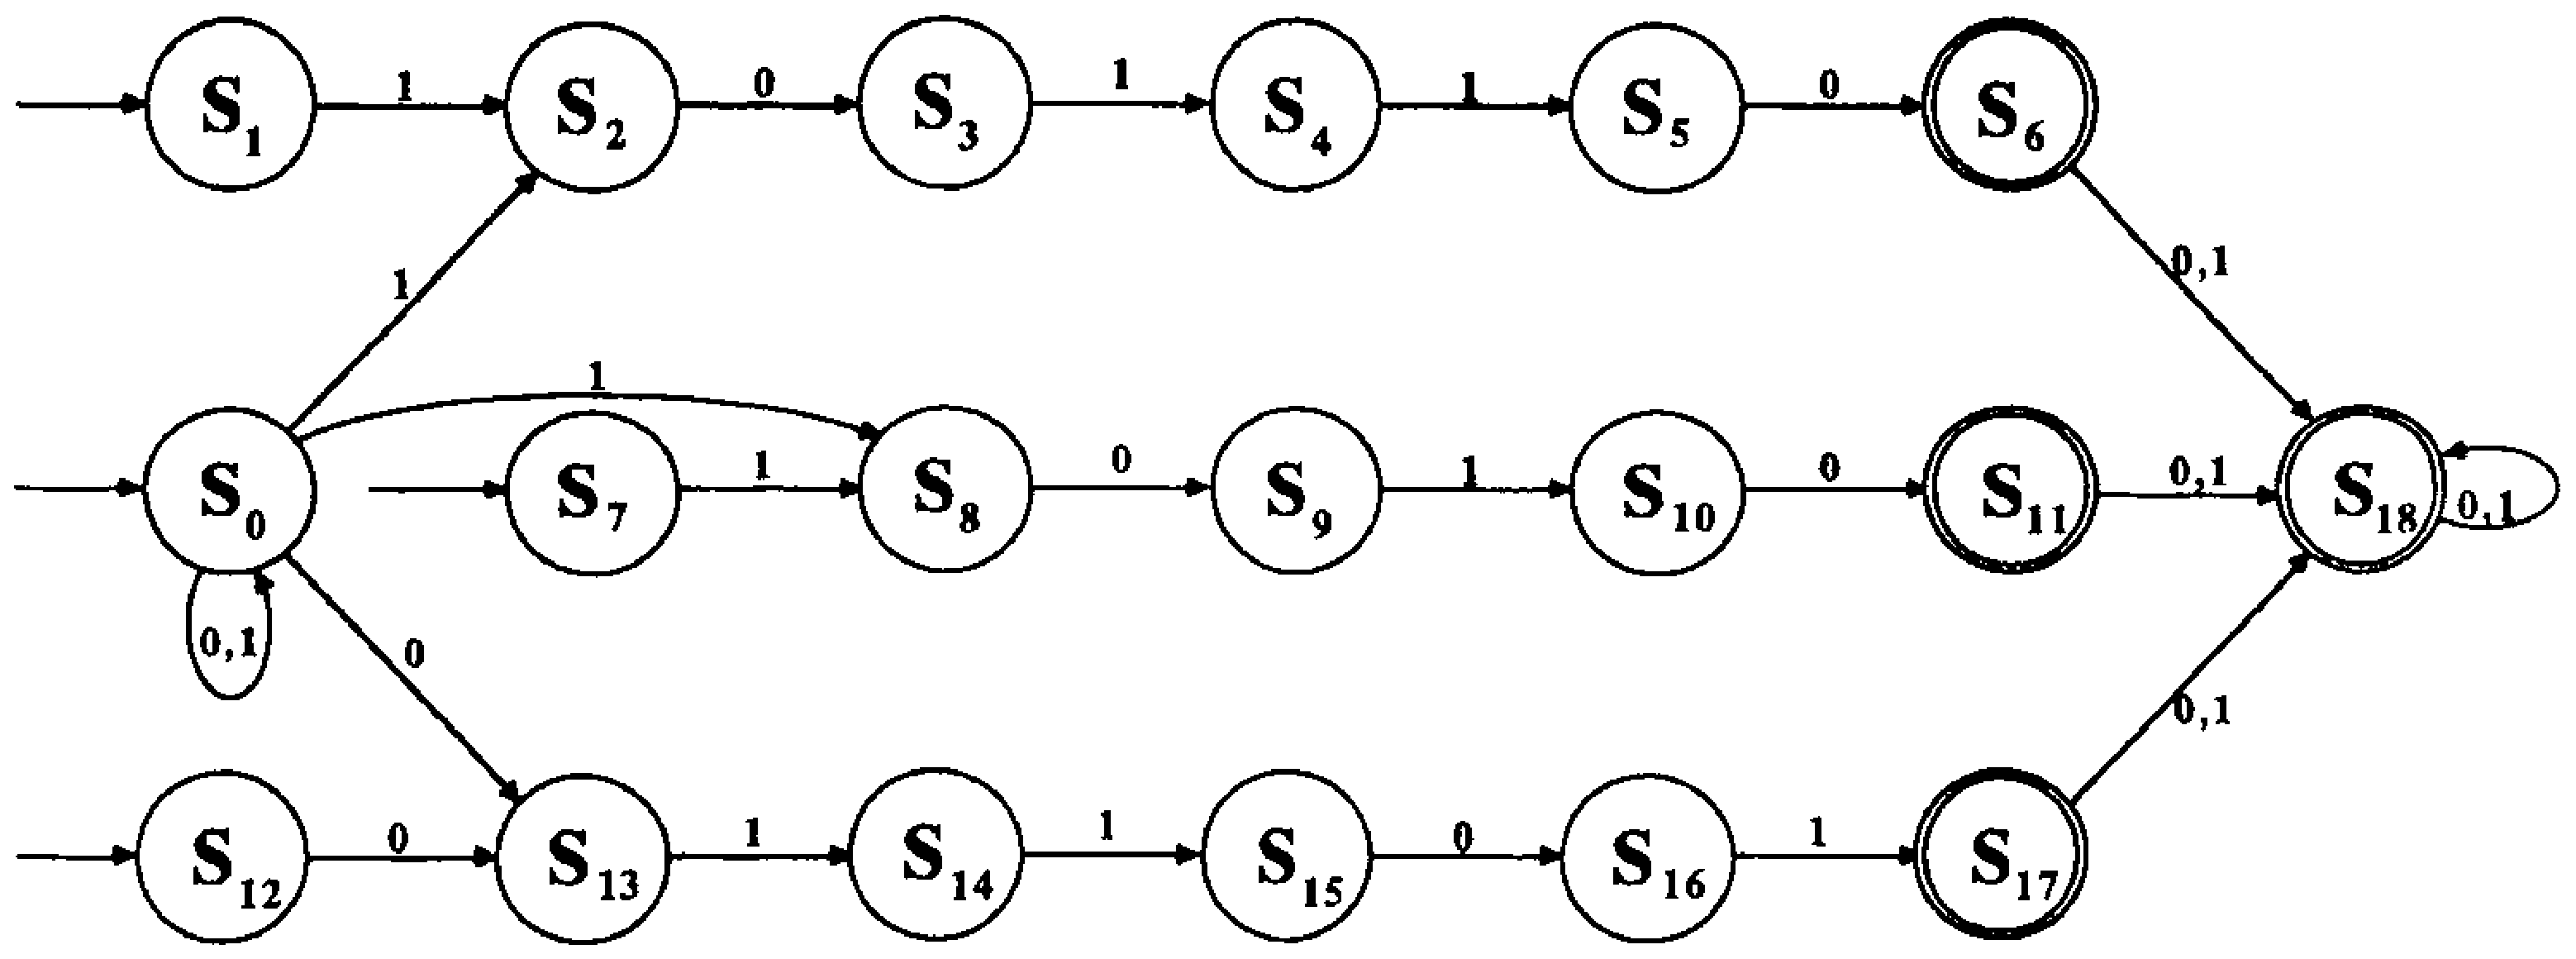
\epsfig{figure=ToFAfigures/fig4-12.eps,width=6.5in}}
\caption{An NDFA for recognizing any of several substrings}\label{fig-4.12}
\end{figure}

\subsection*{Example 4.12}

Recall the application in Chapter \ref{ch-1} involving string searching (Example
1.15). The construction of DFAs involved much thought, but there is an
NDFA that solves the problem in an obvious and straightforward manner. For
example, an automaton that recognizes all strings over the alphabet $\{\pmb{a},
\pmb{b}\}$ containing the substring $\pmb{aab}$ might look like the NDFA in
Figure \ref{fig-4.13}.

% Figure 4.13
\begin{figure}
\centerline{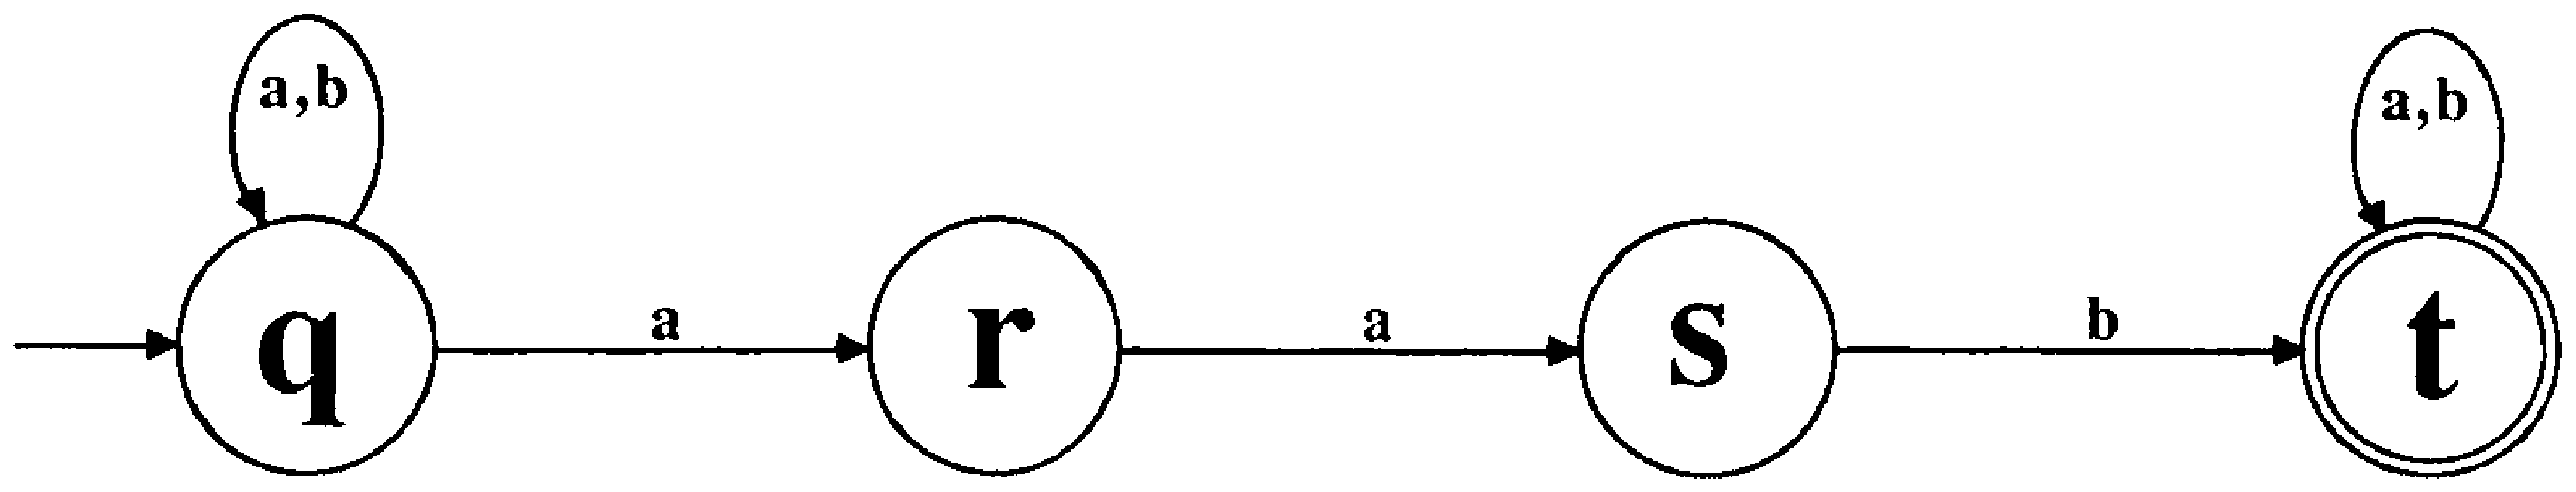
\epsfig{figure=ToFAfigures/fig4-13.eps,width=6.5in}}
\caption{An automaton recognizing the substring $\pmb{aab}$}\label{fig-4.13}
\end{figure}

As is the case for this NDFA, it may be impossible for certain sets of states
to all be active at once. These combinations can never be achieved during the
normal operation of the NDFA. The DFA states corresponding to these combinations
will not be in the connected part of $A^d$. Applying Definition \ref{dfn-4.5} to find the
entire deterministic version and then pruning it down to just the relevant
portion is very inefficient. A better solution is to begin at the start state
and ``follow transitions'' to new states until no further new states are
uncovered. At this point, the relevant states and their transitions will have
all been defined; the remainder of the machine can be safely ignored. For the
NDFA in Figure \ref{fig-4.13}, the connected portion of the equivalent DFA is shown in
Figure \ref{fig-4.14}. This automaton is still not reduced; the last three states are all
equivalent and can be coalesced to form the minimal machine given in Figure \ref{fig-4.15}.

% Figure 4.14
\begin{figure}
\centerline{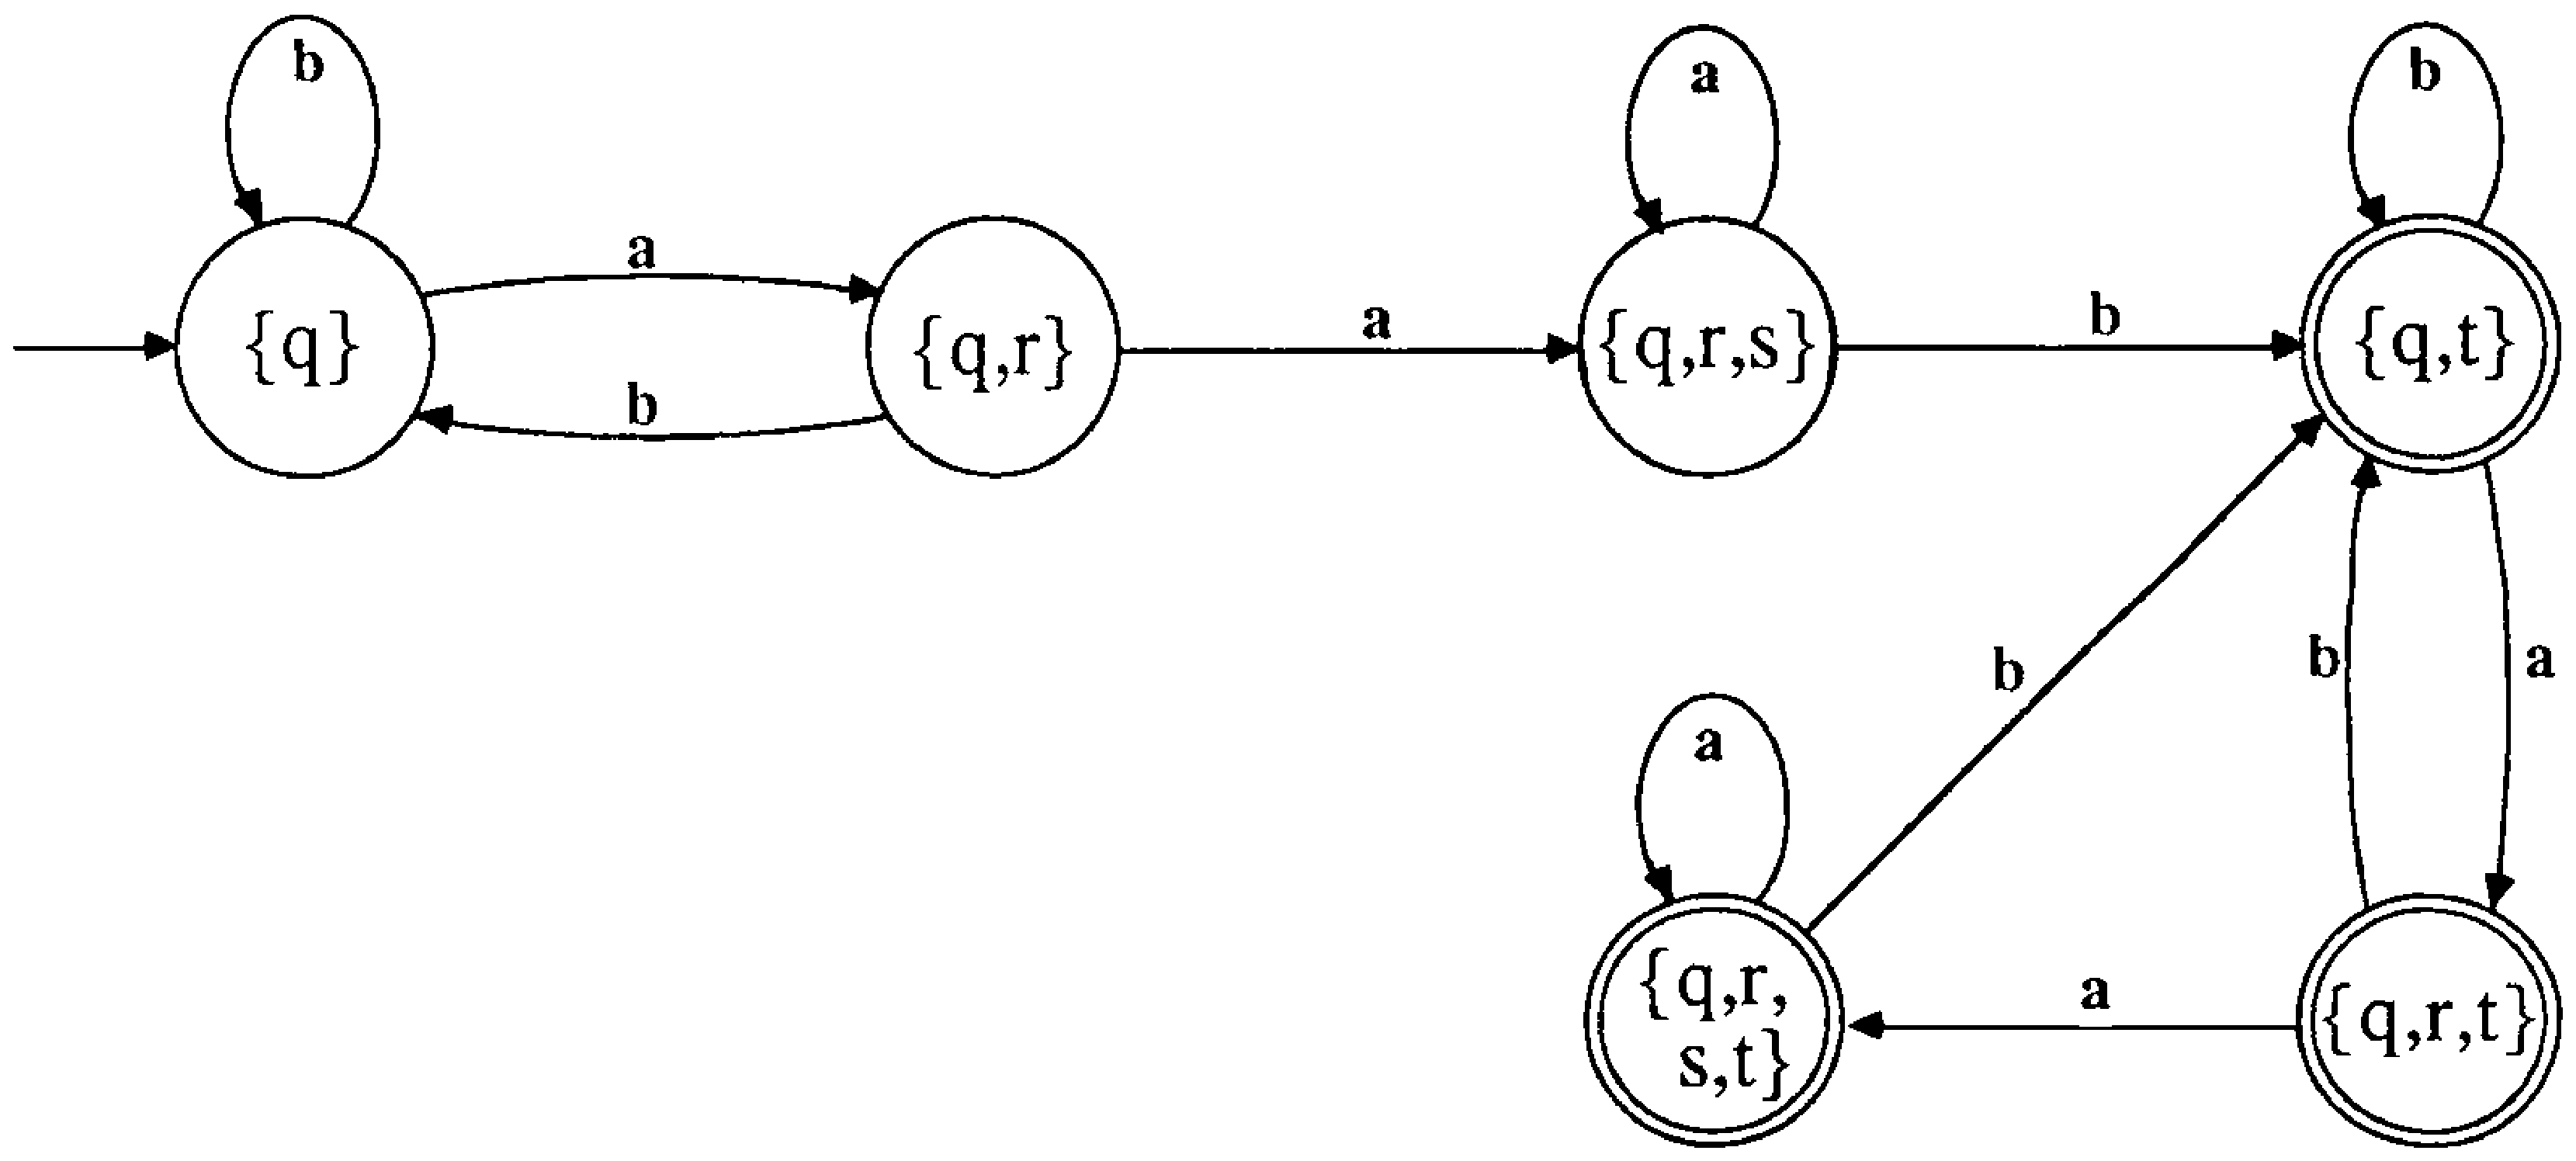
\epsfig{figure=ToFAfigures/fig4-14.eps,width=6.5in}}
\caption{The connected portion of the DFA equivalent to the NDFA given in
Example 4.12}\label{fig-4.14}
\end{figure}

% Figure 4.15
\begin{figure}
\centerline{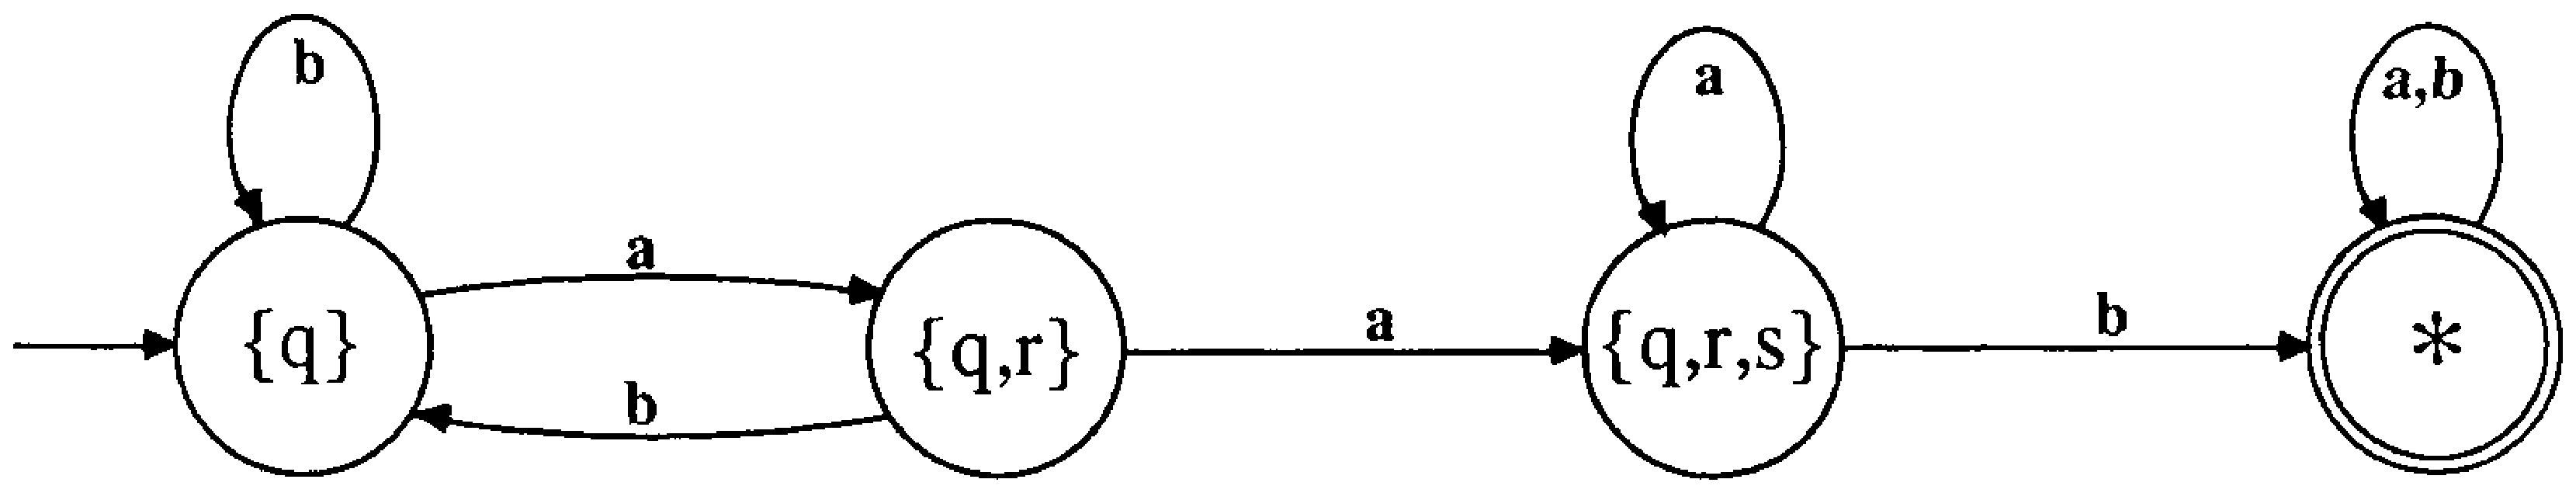
\epsfig{figure=ToFAfigures/fig4-15.eps,width=6.5in}}
\caption{A reduced equivalent of the DFA given in Figure \ref{fig-4.14}}\label{fig-4.15}
\end{figure}

The above process can be easily automated; an interesting but frustrating
exercise might involve producing an appropriate set of rules for generating,
given a specific string $y$, a DFA that will recognize all strings containing
the substring $y$. Definition \ref{dfn-4.5} can be used to generate the appropriate DFA
from the obvious NDFA without subjecting the designer to such frustrations!

\section{Circuit Implementation of NDFAs}\label{sec-4.2}

As mentioned earlier, the presence of multiple paths within an NDFA for a single
word characterizes the nondeterministic nature of these automata. The most
profitable way to view the operation of an NDFA is to consider the automaton as
having (potentially) several active states, with each of the active states
reacting to the next letter to determine a new set of active states. In fact, by
using one D flip-flop per state, this viewpoint can be directly translated into
hardware. When a given state is active, the corresponding flip-flop will be on,
and when it is inactive (that is, it cannot be reached by the substring that has
been processed at this point), it will be off. As a new letter is processed, a
state will be activated (that is, be placed in the new set of active states) if
it can be reached from one of the previously active states. Thus, the state
transition function will again determine the circuitry that feeds into each
flip-flop.

Following the same conventions given for DFAs, the input tape will be assumed
to be bounded by special start-of-string \<SOS\> and end-of-string \<EOS\>
symbols. The \<EOS\> character is again used to activate the accept circuitry
so that acceptance is not indicated until all letters on the tape have been
processed. As before, the \<SOS\> symbol can be employed at the beginning of the
string to ensure that the circuitry begins processing the string from the
appropriate start state(s). Alternately, SR (set-reset) flip-flops can be used
to initialize the configuration without relying on the <SOS> conventions.

\subsection*{Example 4.13}

Consider the NDFA $D$ given in Figure \ref{fig-4.16}. With the \<SOS\> and \<EOS\>
transitions illustrated, the complete model would appear as in Figure \ref{fig-4.17}.

Two bits of input data ($\pmb{a}_1$ and $\pmb{a}_2$) are required to represent
the symbols \<EOS\>, $\pmb{a}$, $\pmb{b}$, and \<SOS\>. The standard encodings
described in Chapter \ref{ch-1} would produce \<EOS\> $=\pmb{00},\pmb{a}=\pmb{01},\pmb{b}
=\pmb{10}$, and \<SOS\> $=\pmb{11}$. If the flip-flop $t_1$ is used to represent
the activity of $s_1$, and $t_2$ is used to record the status of $s_2$, then
the subsequent activity of the two flip-flops can be determined from the current
state activity and the current letter being scanned, as shown in Table \ref{tbl-4.1}.

% Figure 4.16
\begin{figure}
\centerline{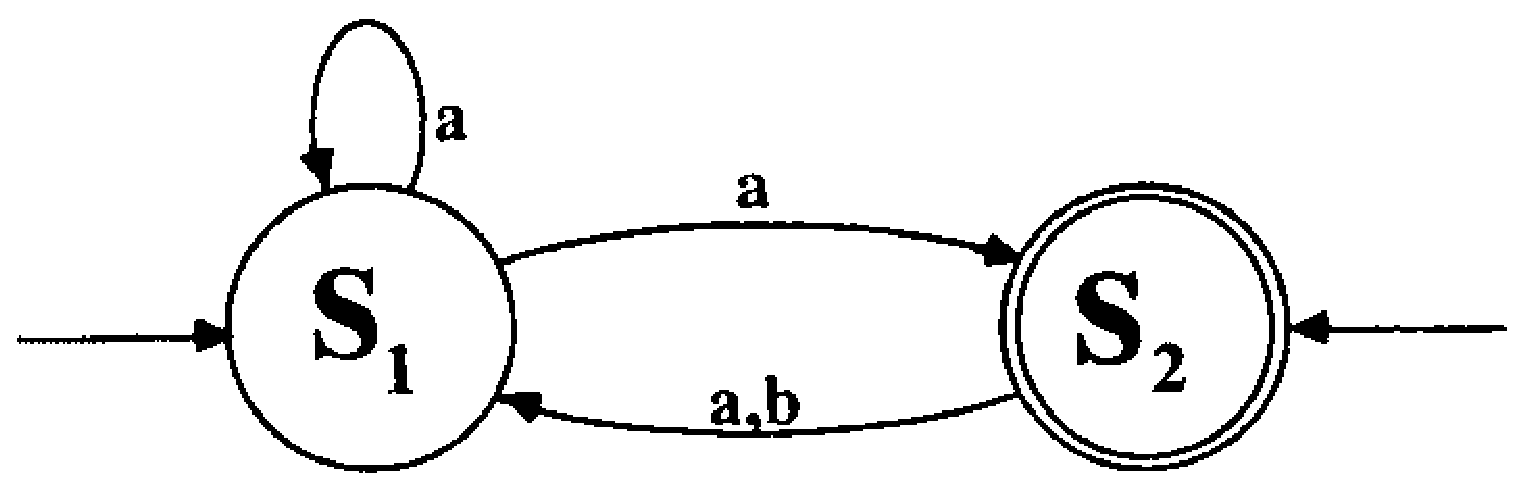
\epsfig{figure=ToFAfigures/fig4-16.eps,width=2.5in}}
\caption{The NDFA discussed in Example 4.13}\label{fig-4.16}
\end{figure}
% Figure 4.17
\begin{figure}
\centerline{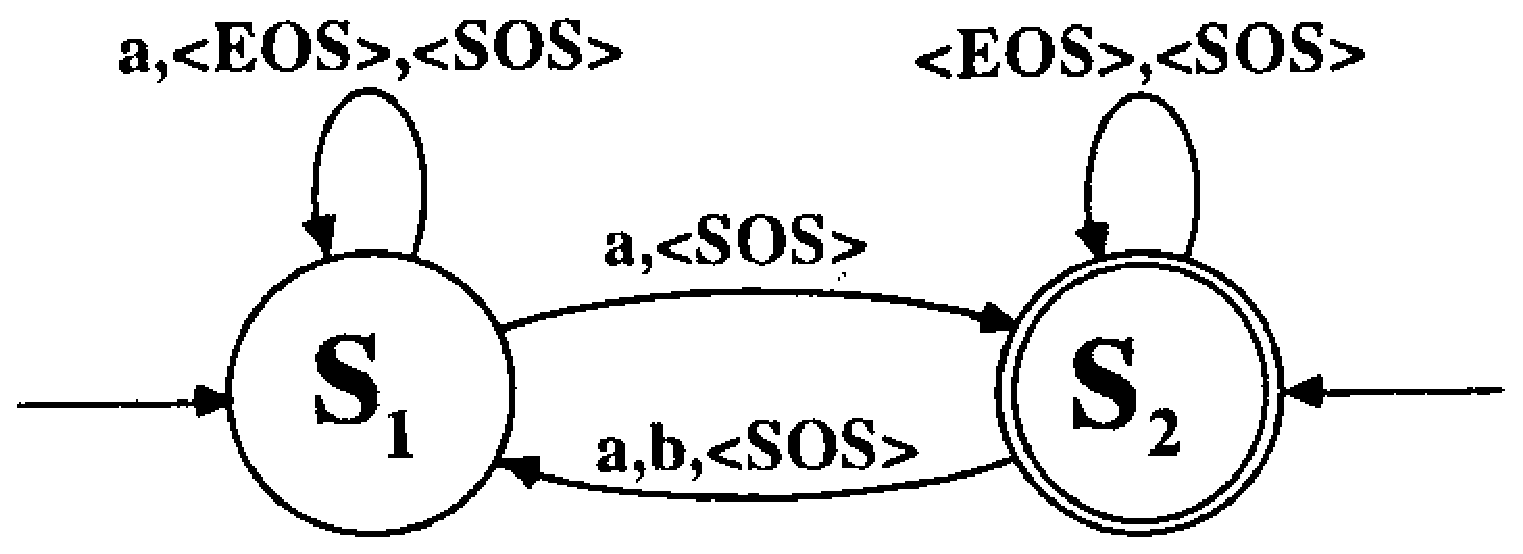
\epsfig{figure=ToFAfigures/fig4-17.eps,width=2.5in}}
\caption{The expanded state transition diagram for the NDFA in Figure \ref{fig-4.16}}\label{fig-4.17}
\end{figure}

% Table 4.1
\begin{table}[h]
\caption{}\label{tbl-4.1}
\begin{center}\begin{tabular}{cccc|ccc}
$t_1$ & $t_2$ & $a_1$ & $a_2$ & $t'_1$ & $t'_2$ & {\bf accept} \\
\hline
$\pmb{0}$ & $\pmb{0}$ & $\pmb{0}$ & $\pmb{0}$ & $\pmb{0}$ & $\pmb{0}$ &
	$\pmb{0}$ \\
$\pmb{0}$ & $\pmb{0}$ & $\pmb{0}$ & $\pmb{1}$ & $\pmb{0}$ & $\pmb{0}$ &
	$\pmb{0}$ \\
$\pmb{0}$ & $\pmb{0}$ & $\pmb{1}$ & $\pmb{0}$ & $\pmb{0}$ & $\pmb{0}$ &
	$\pmb{0}$ \\
$\pmb{0}$ & $\pmb{0}$ & $\pmb{1}$ & $\pmb{1}$ & $\pmb{1}$ & $\pmb{1}$ &
	$\pmb{0}$ \\
$\pmb{0}$ & $\pmb{1}$ & $\pmb{0}$ & $\pmb{0}$ & $\pmb{0}$ & $\pmb{1}$ &
	$\pmb{1}$ \\
$\pmb{0}$ & $\pmb{1}$ & $\pmb{0}$ & $\pmb{1}$ & $\pmb{1}$ & $\pmb{0}$ &
	$\pmb{0}$ \\
$\pmb{0}$ & $\pmb{1}$ & $\pmb{1}$ & $\pmb{0}$ & $\pmb{1}$ & $\pmb{0}$ &
	$\pmb{0}$ \\
$\pmb{0}$ & $\pmb{1}$ & $\pmb{1}$ & $\pmb{1}$ & $\pmb{1}$ & $\pmb{1}$ &
	$\pmb{0}$ \\
$\pmb{1}$ & $\pmb{0}$ & $\pmb{0}$ & $\pmb{0}$ & $\pmb{1}$ & $\pmb{0}$ &
	$\pmb{0}$ \\
$\pmb{1}$ & $\pmb{0}$ & $\pmb{0}$ & $\pmb{1}$ & $\pmb{1}$ & $\pmb{1}$ &
	$\pmb{0}$ \\
$\pmb{1}$ & $\pmb{0}$ & $\pmb{1}$ & $\pmb{0}$ & $\pmb{0}$ & $\pmb{0}$ &
	$\pmb{0}$ \\
$\pmb{1}$ & $\pmb{0}$ & $\pmb{1}$ & $\pmb{1}$ & $\pmb{1}$ & $\pmb{1}$ &
	$\pmb{0}$ \\
$\pmb{1}$ & $\pmb{1}$ & $\pmb{0}$ & $\pmb{0}$ & $\pmb{1}$ & $\pmb{1}$ &
	$\pmb{1}$ \\
$\pmb{1}$ & $\pmb{1}$ & $\pmb{0}$ & $\pmb{1}$ & $\pmb{1}$ & $\pmb{1}$ &
	$\pmb{0}$ \\
$\pmb{1}$ & $\pmb{1}$ & $\pmb{1}$ & $\pmb{0}$ & $\pmb{1}$ & $\pmb{0}$ &
	$\pmb{0}$ \\
$\pmb{1}$ & $\pmb{1}$ & $\pmb{1}$ & $\pmb{1}$ & $\pmb{1}$ & $\pmb{1}$ &
	$\pmb{0}$
\end{tabular}\end{center}
\end{table}

The first four rows of Table \ref{tbl-4.1} reflect the situation in which a string is
hopelessly stuck, and no states are active. Processing subsequent symbols from
$\Sigma$, will not change this; both $t'_1$ and $t'_2$ remain $\pmb{0}$. The one
exception is when the \<SOS\> symbol is scanned; in this case, each of the start
states is activated ($t'_1 = \pmb{1}$ and $t'_2 = \pmb{1}$). This corrects the
situation in which both flip-flops happen to initialize to $\pmb{0}$ when power
is first applied to the circuitry. Scanning the \<SOS\> symbol changes the state
of the flip-flops to reflect the appropriate starting conditions (in this
machine, both states are start states, and therefore both should be active as
processing is begun). Note that each of the rows of Table \ref{tbl-4.1} that correspond to
scanning \<SOS\> show that $t_1$ and $t_2$ are reset in the same fashion.

Determining the circuit behavior for the symbols in $\Sigma$, closely parallels
the definition of $\delta^d$ in Definition \ref{dfn-4.5}. For example, when state $s_1$ is
active but $s_2$ is inactive $(t_1=\pmb{1}$ and $t_2=\pmb{0})$ and $\pmb{a}$ is
scanned $(\pmb{a}_1=\pmb{0}$ and $\pmb{a}_2=\pmb{1})$, transitions from $s_1$
cause both states to next be active ($t'_1=\pmb{1}$ and $t'_2=\pmb{1}$). The
other combinations are calculated similarly. Minimized expressions for the new
values of each of the flip-flops and the accept circuitry are:
\begin{center}\begin{tabular}{rcl}
$t'_1$ & $=$ & $(t_1\wedge\neg\pmb{a}_1) \vee (t_2\wedge\pmb{a}_2) \vee
	(t_2\wedge\pmb{a}_1) \vee (\pmb{a}_1\wedge\pmb{a}_2)$ \\
$t'_2$ & $=$ & $(t_2\wedge\neg\pmb{a}_1\wedge\neg\pmb{a}_2) \vee
	(t_1\wedge\pmb{a}_2) \vee (\pmb{a}_1\wedge\pmb{a}_2)$ \\
accept & $=$ & $(t_2\wedge\neg\pmb{a}_1\wedge\neg\pmb{a}_2)$
\end{tabular}\end{center}
Since similar terms appear in these expressions, these three subcircuits can
``share'' the common components, as shown in Figure \ref{fig-4.18}.

% Figure 4.18
\begin{figure}
\centerline{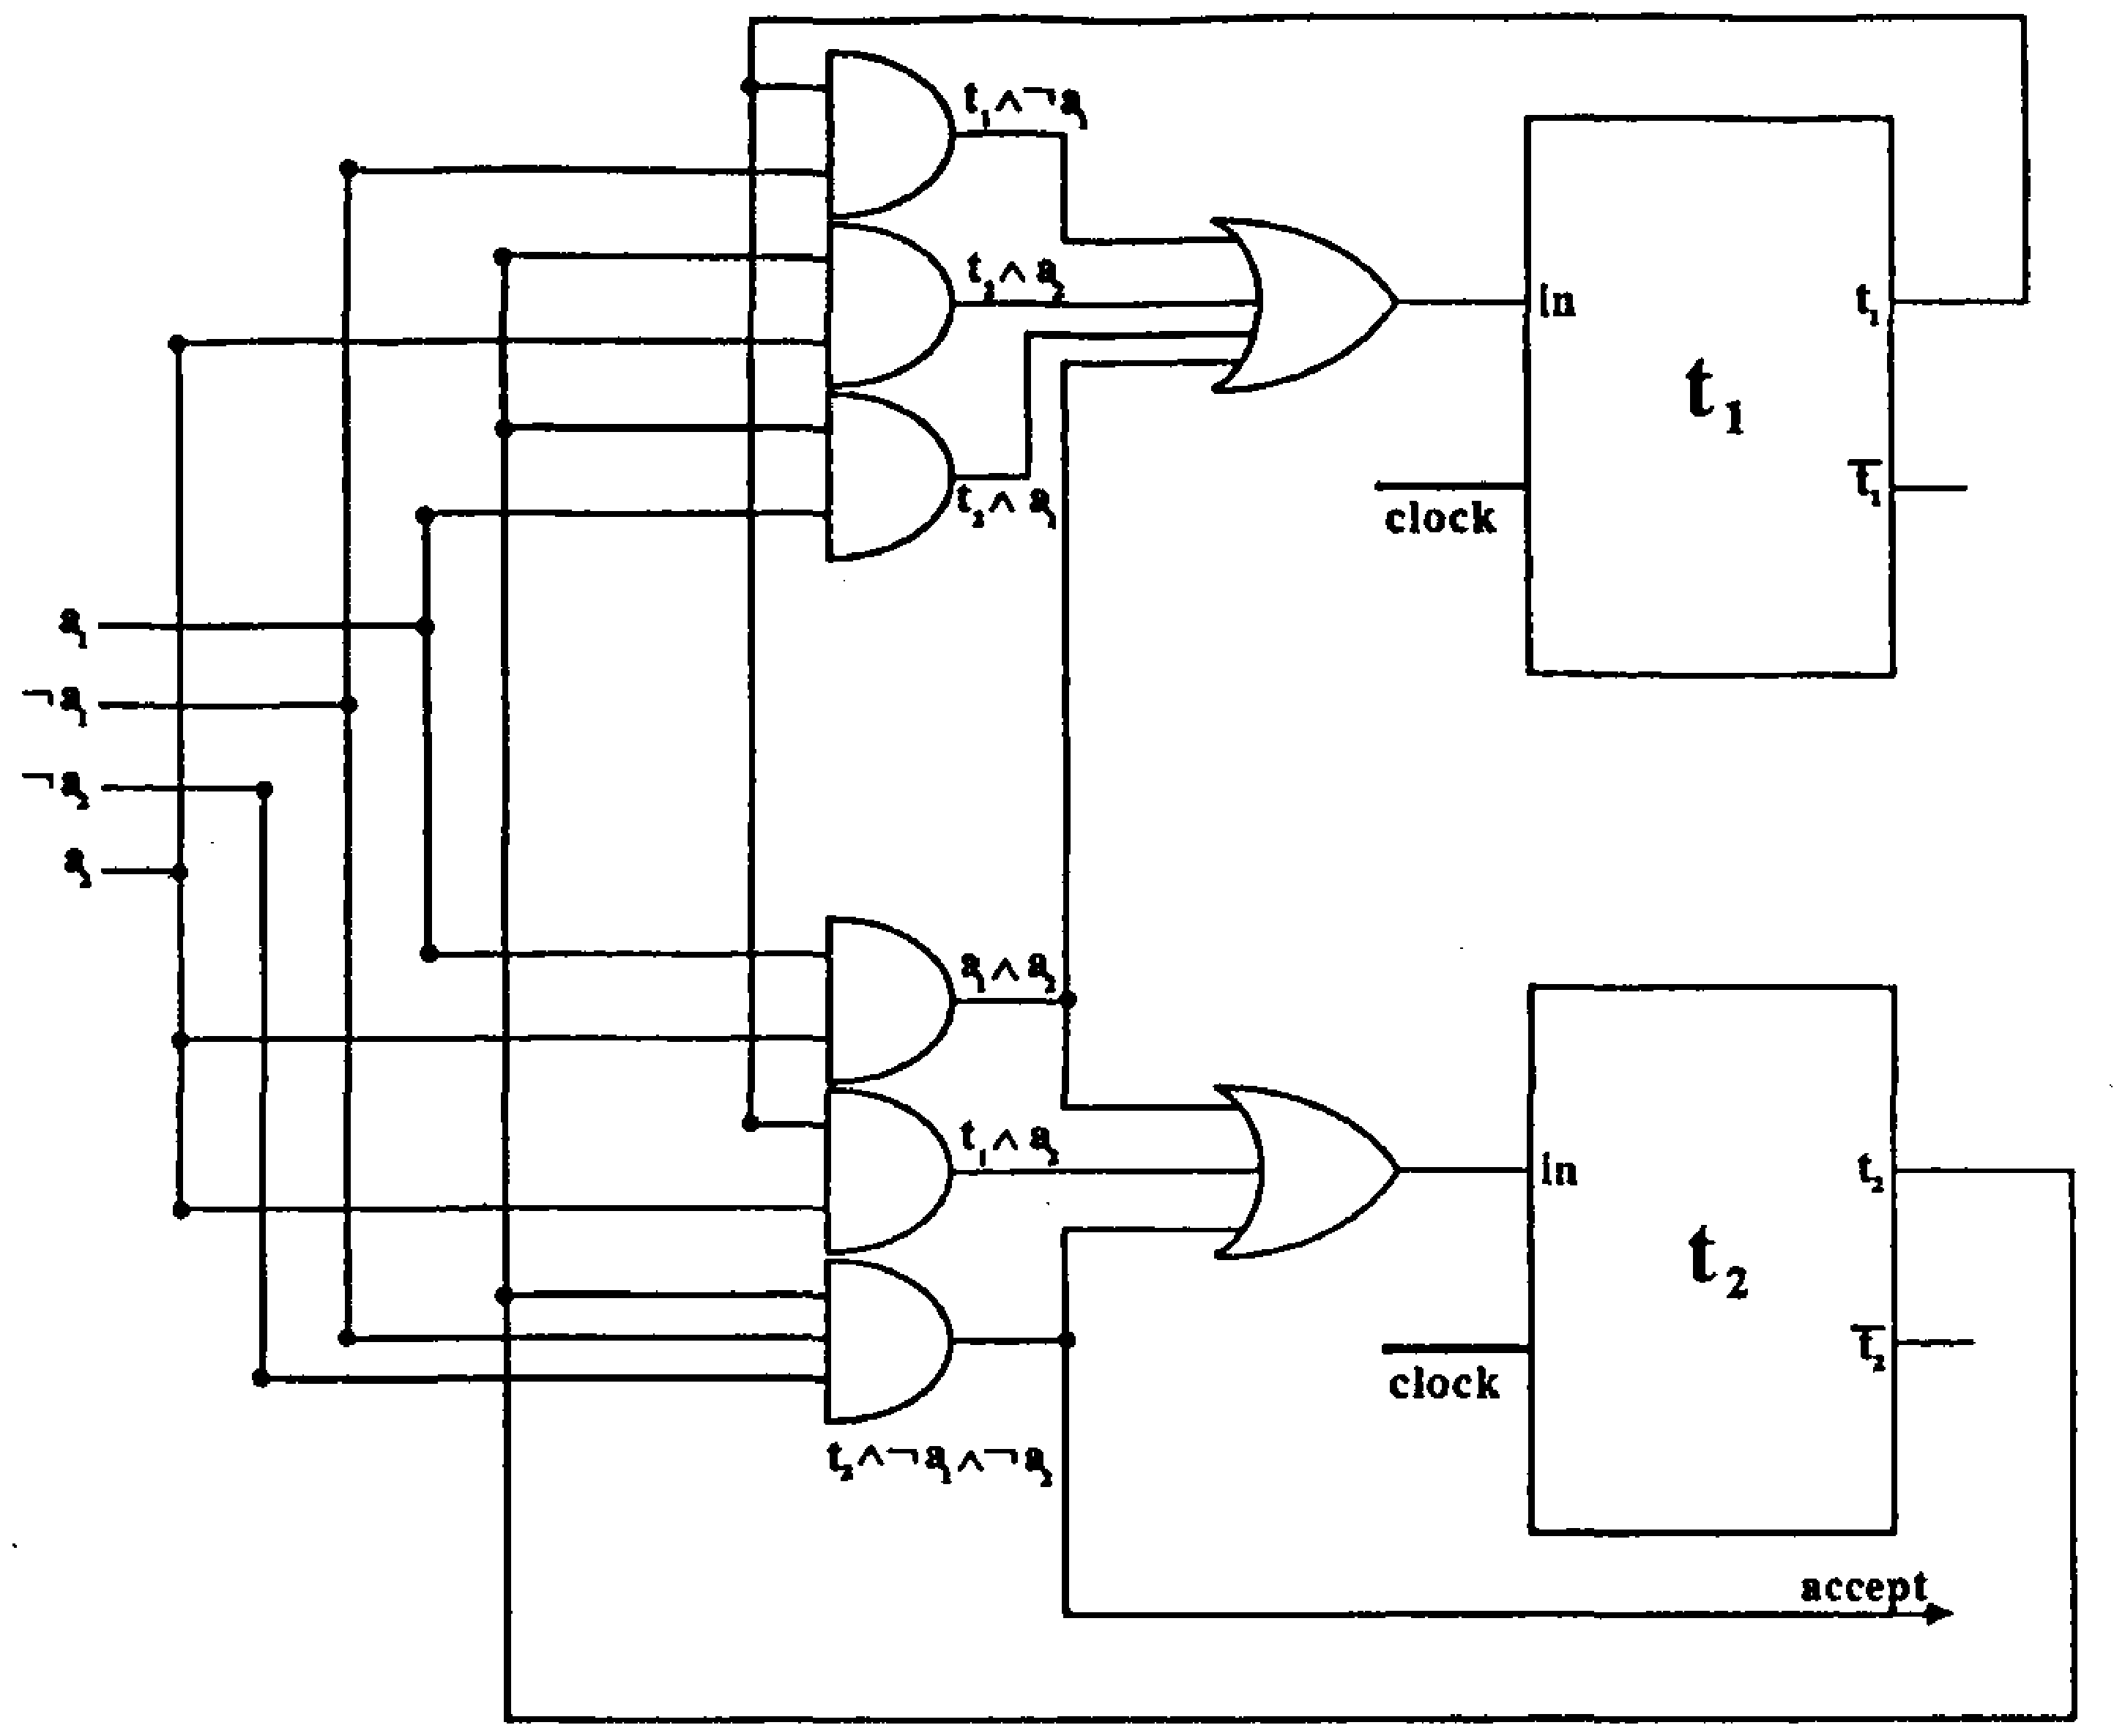
\epsfig{figure=ToFAfigures/fig4-18.eps,width=6in}}
\caption{Circuitry for the automaton discussed in Example 4.13}\label{fig-4.18}
\end{figure}

Note that the accept circuitry reflects that a string should be recognized when
some final state is active ($s_2$ in this example) and \<EOS\> is scanned. In
more complex machines with several final states, lines leading from each of the
flip-flops corresponding to final states would be joined by an OR gate
before being ANDed with the \<EOS\> condition.

An interesting exercise involves converting the NDFA $D$ given in Example 4.1
to the equivalent DFA $D^d$, which will have four states: $\emptyset,\ \{s_1\},\
\{s_2\}$, and $\{s_1,s_2\}$. The deterministic automaton $D^d$ can be realized
by a circuit diagram as specified in Chapter \ref{ch-1}. This four-stare DFA will require
2 bits of state data. If the state encoding conventions $\emptyset=\pmb{00}$,
$\{s_1\}=\pmb{10}$, $\{s_2\}=\pmb{01}$, and $\{s_1,s_2\}=\pmb{11}$ are used, the
circuitry for the DFA $D^d$ will be identical to that for the NDFA $D$.

For DFAs, $m$ bits of state data ($t_1,t_2, \ldots ,t_m)$ can encode up to $2^m$
distinct states. With NDFAs, an $n$-state machine required a full $n$ bits of
state data (1 bit per state). This apparently ``extravagant'' use of state data
is offset by the fact that an $n$-state NDFA may require $2^n$ states to form an
equivalent DFA. This was the case in the preceding example, in which $n$ and $m$
were equal to 2; the two-state NDFA $D$ required two flip-flops, and the
equivalent four-state DFA also required two flip-flops; the savings induced by
the DFA state encoding was exactly offset by the multiplicity of states needed
by the NDFA.

A DFA may turn out to need less hardware than an equivalent NDFA, as illustrated
by Example 4.12. The four-state NDFA $C$ needs four flip-flops, and the
(nonminimal, 16-state) DFA $C^d$ would also need four. However, the minimal
equivalent DFA derived in Example 4.12 has only four states and therefore can be
encoded with just 2 bits of state data. Hence only two flip-flops are necessary
to implement a recognizer for $L(C)$.

\section{NDFAs With Lambda-Transitions}\label{sec-4.3}

We now extend our computational model to include the nondeterministic finite
automata that allow transitions between states to occur ``spontaneously,''
without any input being processed. A transition that occurs without an input
symbol being processed is called a \emph{$\lambda$-transition} or
\emph{lambda-move}\index{lambda-move|see|{$\lambda$-transition}}. In texts that denote the empty string by the symbol
$\epsilon$, such a transition is usually referred to as an
\emph{$\epsilon$-move}\index{$\epsilon$-move|see{$\lambda$-transition}}.

% Definition 4.6
\begin{dfn}\label{dfn-4.6}\index{L@$\lambda$-transition}
A \emph{nondeterministic finite automaton with $\lambda$-transitions} is a
quintuple $A_{\lambda}=\langle\Sigma,S,S_0,\delta_{\lambda},F\rangle$, where
\begin{enumerate}[i.]
\item $\Sigma$ is an alphabet.
\item $S$ is a finite nonempty set of states.
\item $S_0$ is a set of initial states,\index{start state} a nonempty subset of $S$.
\item $\delta_{\!\lambda}:\ (S \times (\Sigma\cup\{\lambda\})) \rightarrow \wp(S)$
	is the state transition function.
\item $F$ is the set of accepting states, a (possibly empty) subset of $S$.
\end{enumerate}
\end{dfn}

A nondeterministic finite automaton \emph{with} $\lambda$-transitions is very
similar in structure to an NDFA that does not have $\lambda$-transitions. The
only different aspect is the definition of the $\delta$ function. Instead of
mapping state/letter pairs [from $S \times \Sigma$] to $\wp(S)$, it maps pairs
consisting of a state and either a letter or the empty string [from $S \times
(\Sigma\cup\{\lambda\})$ to $\wp(S)$]. From any state that has a
$\lambda$-transition, we adopt the convention that the machine is capable of
making a spontaneous transition to the new state specified by that
$\lambda$-transition \emph{without} processing an input symbol. However, the
machine may also ``choose'' not to follow this path and instead remain in the
original state. Before we can extend the $\delta_{\lambda}$ function to operate
on strings from $\Sigma^*$, we need the very useful concept of
\emph{lambda-closure}\index{lambda-closure|see{$\lambda$-closure}}.

% Definition 4.7
\begin{dfn}\label{dfn-4.7}\index{L@$\lambda$-closure}
Given a nondeterministic finite automaton
\[ A_{\lambda} = \langle\Sigma,S,S_0,\delta_{\lambda},F\rangle \]
with $\lambda$-transitions, the \emph{$\lambda$-closure of a state} $t \in S$,
denoted $\Lambda(t)$, is the set of all states that are reachable from $t$
without processing any input symbols. The \emph{$\lambda$-closure of a
set of states $T$} is then $\Lambda(T) = \bigcup\limits_{t\,\in\, T} \Lambda(t)$.
\end{dfn}

The $\lambda$-closure of a state is the set of all the states that can be
reached from that state, including itself, by following $\lambda$-transitions only.
Obviously, one can always reach the state currently occupied without having to
move. Consequently, even if there are no explicit arcs labeled by $\lambda$
going back to state $t$, $t$ is always in the $\lambda$-closure of itself.

\subsection*{Example 4.14}

Consider the machine given in Figure \ref{fig-4.19}, which contains $\lambda$-transitions
from $s_0$ to $s_1$ and from $s_1$ to $s_2$. By Definition \ref{dfn-4.7},
\begin{center}\begin{tabular}{l}
$\Lambda(s_0) = \{s_0,s_1,s_2\}$ \\
$\Lambda(s_1) = \{s_1,s_2\}$ \\
$\Lambda(s_2) = \{s_2\}$ \\
$\Lambda(s_3) = \{s_3\}$
\end{tabular}\end{center}

% Figure 4.19
\begin{figure}
\centerline{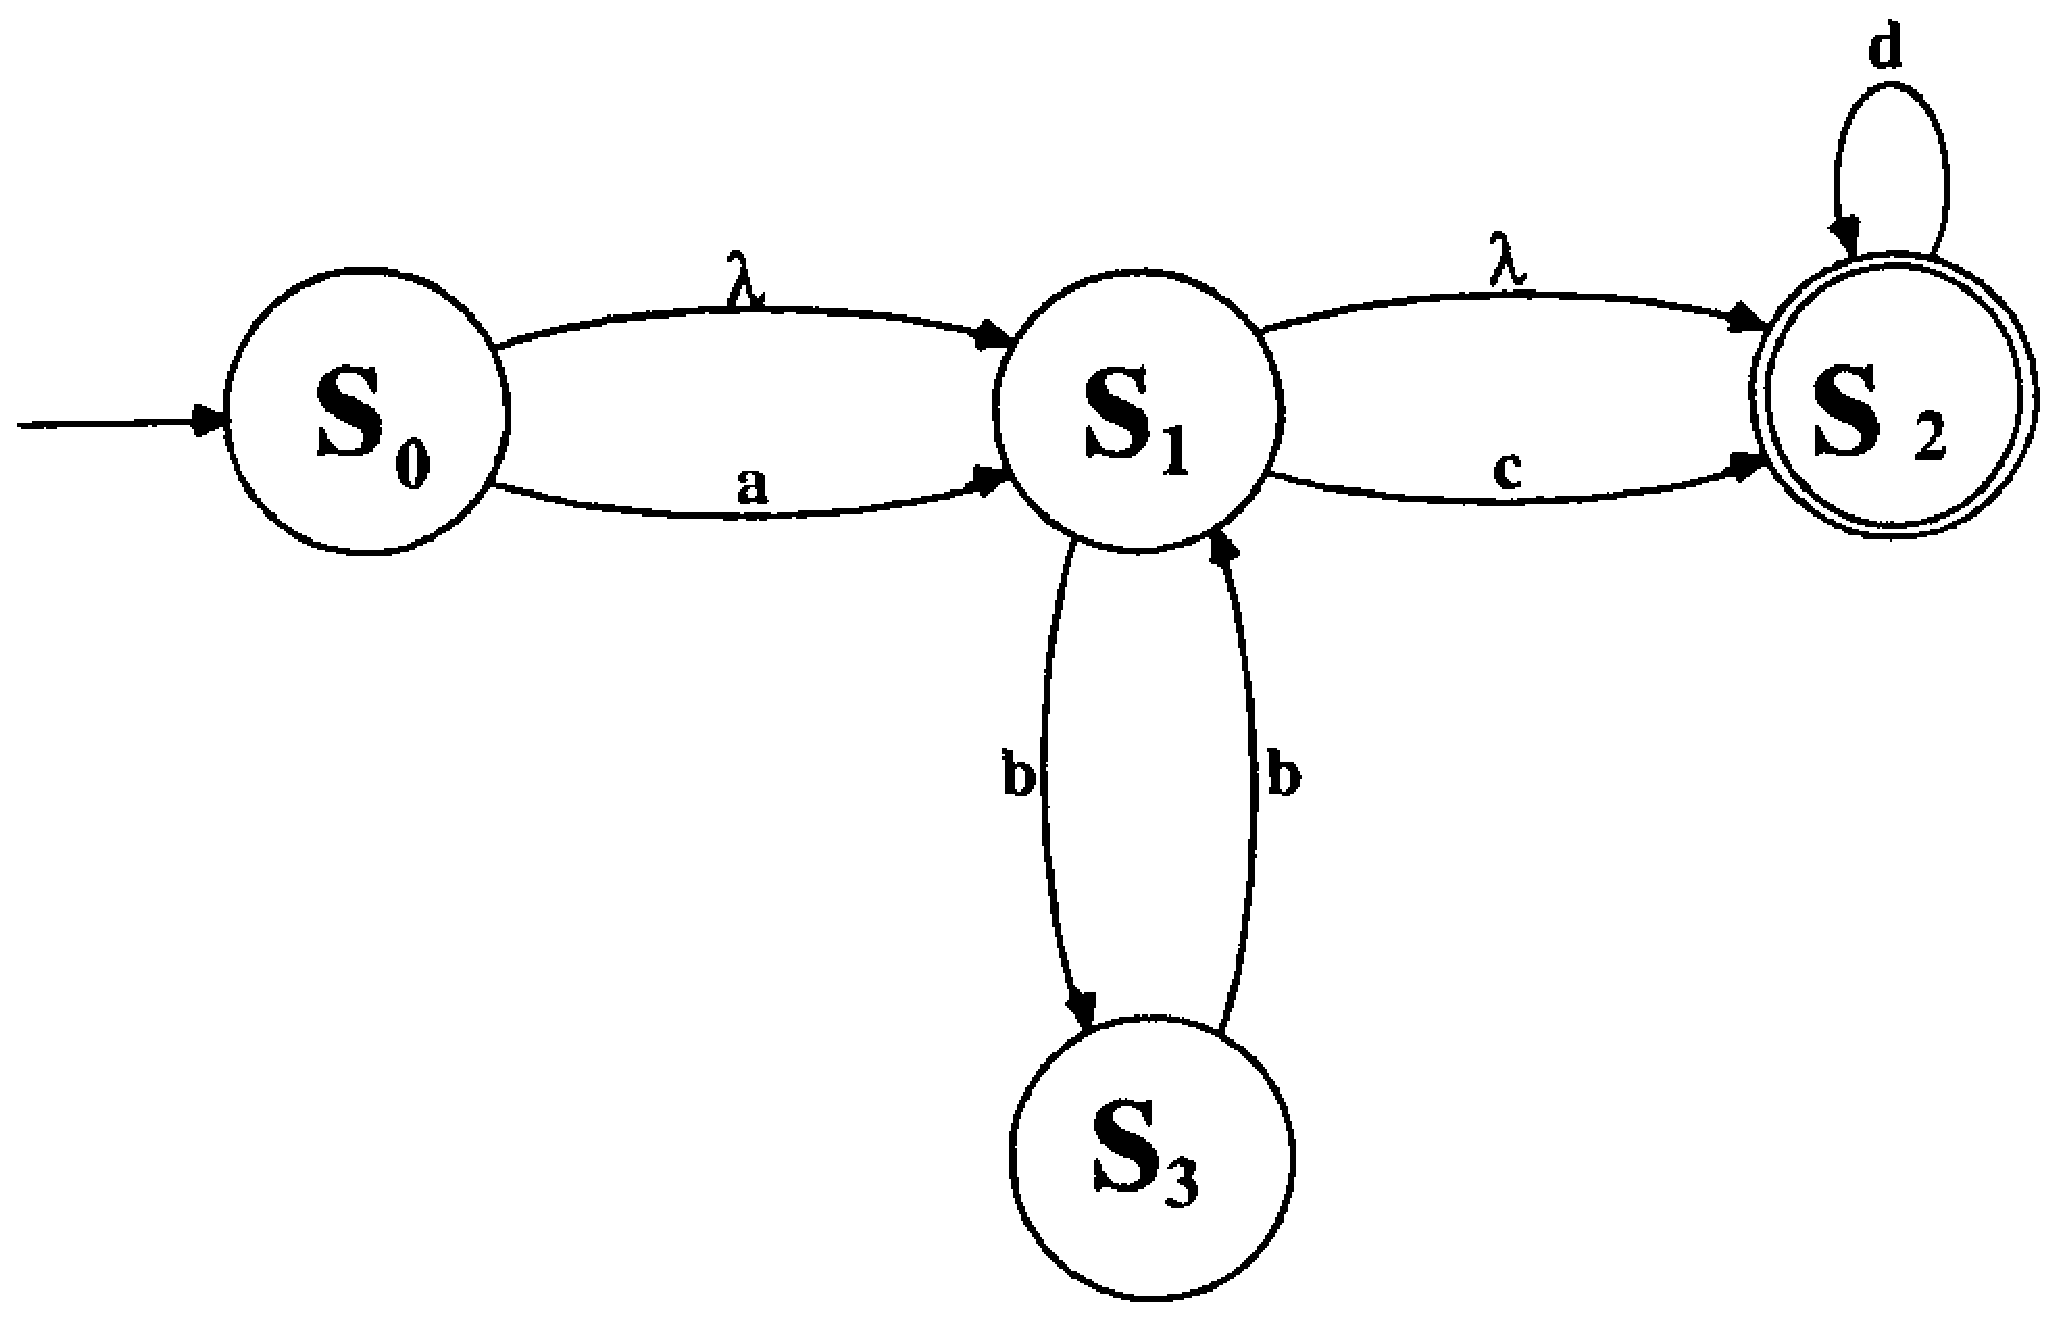
\epsfig{figure=ToFAfigures/fig4-19.eps,width=3.5in}}
\caption{An NDFA with lambda-moves}\label{fig-4.19}
\end{figure}

% Definition 4.8
\begin{dfn}\label{dfn-4.8}\index{extended state transition function \DBAR\! for NDFA $A_{\lambda}$}\index{state transition function!for NDFA $A_{\lambda}$}
Given a nondeterministic finite automaton
\[ A_{\lambda} = \langle\Sigma,S,S_0,\delta_{\lambda},F\rangle \]
with $\lambda$-transitions, the \emph{extended state transition function
for $A_{\lambda}$} is a function $\DBAR_{\!\lambda}$$: S \times \Sigma^*
\rightarrow \wp(S)$ defined as follows:
\begin{enumerate}[i.]
\item $(\forall s \in S)\DBAR_{\!\lambda}(s,\lambda) = \Lambda(s)$
\item $(\forall s \in S)(\forall\pmb{a}\in\Sigma)\DBAR_{\!\lambda}(s,\pmb{a}) =
	\Lambda( \bigcup\limits_{q\,\in\,\Lambda(s)}\delta_{\!\lambda}(q,\pmb{a}))$
\item $(\forall s \in S)(\forall x \in \Sigma^*)(\forall\pmb{a}\in\Sigma)
	\DBAR_{\!\lambda}(s,x\pmb{a}) = \Lambda(\bigcup\limits_{q\,\in\,\DBAR_{
	\!\lambda}(s,x)} \delta_{\!\lambda}(q,\pmb{a}))$
\end{enumerate}
\end{dfn}

The $\DBAR_{\!\lambda}$ function is \emph{not} extended in the same way as for the
nondeterministic finite automata given in Definition \ref{dfn-4.2}. Most importantly, due
to the effects of the $\lambda$-closure, $\DBAR_{\!\lambda}(s,\pmb{a}) \not=
\delta_{\!\lambda}(s,\pmb{a})$. Thus, not only does the $\DBAR_{\!\lambda}$ function
map to a set of states based on a single letter, but it also includes the
$\lambda$-closure of those states. This may seem strange for single letters
(strings of length 1), but it is required for consistency when the
$\DBAR_{\!\lambda}$ function is presented with strings of length greater than 1,
since at each state along the path there can be $\lambda$-transitions. Each
$\lambda$-transition maps to a new state (which may have $\lambda$-transitions
of its own) that must be included in this path and processed by the
$\delta_{\!\lambda}$ function.

The nondeterministic finite automaton \emph{without} $\lambda$-transitions that
corresponds to a nondeterministic finite automaton \emph{with} $\lambda$-transitions is
given in Definition \ref{dfn-4.9}.

% Figure 4.20
\begin{figure}
\centerline{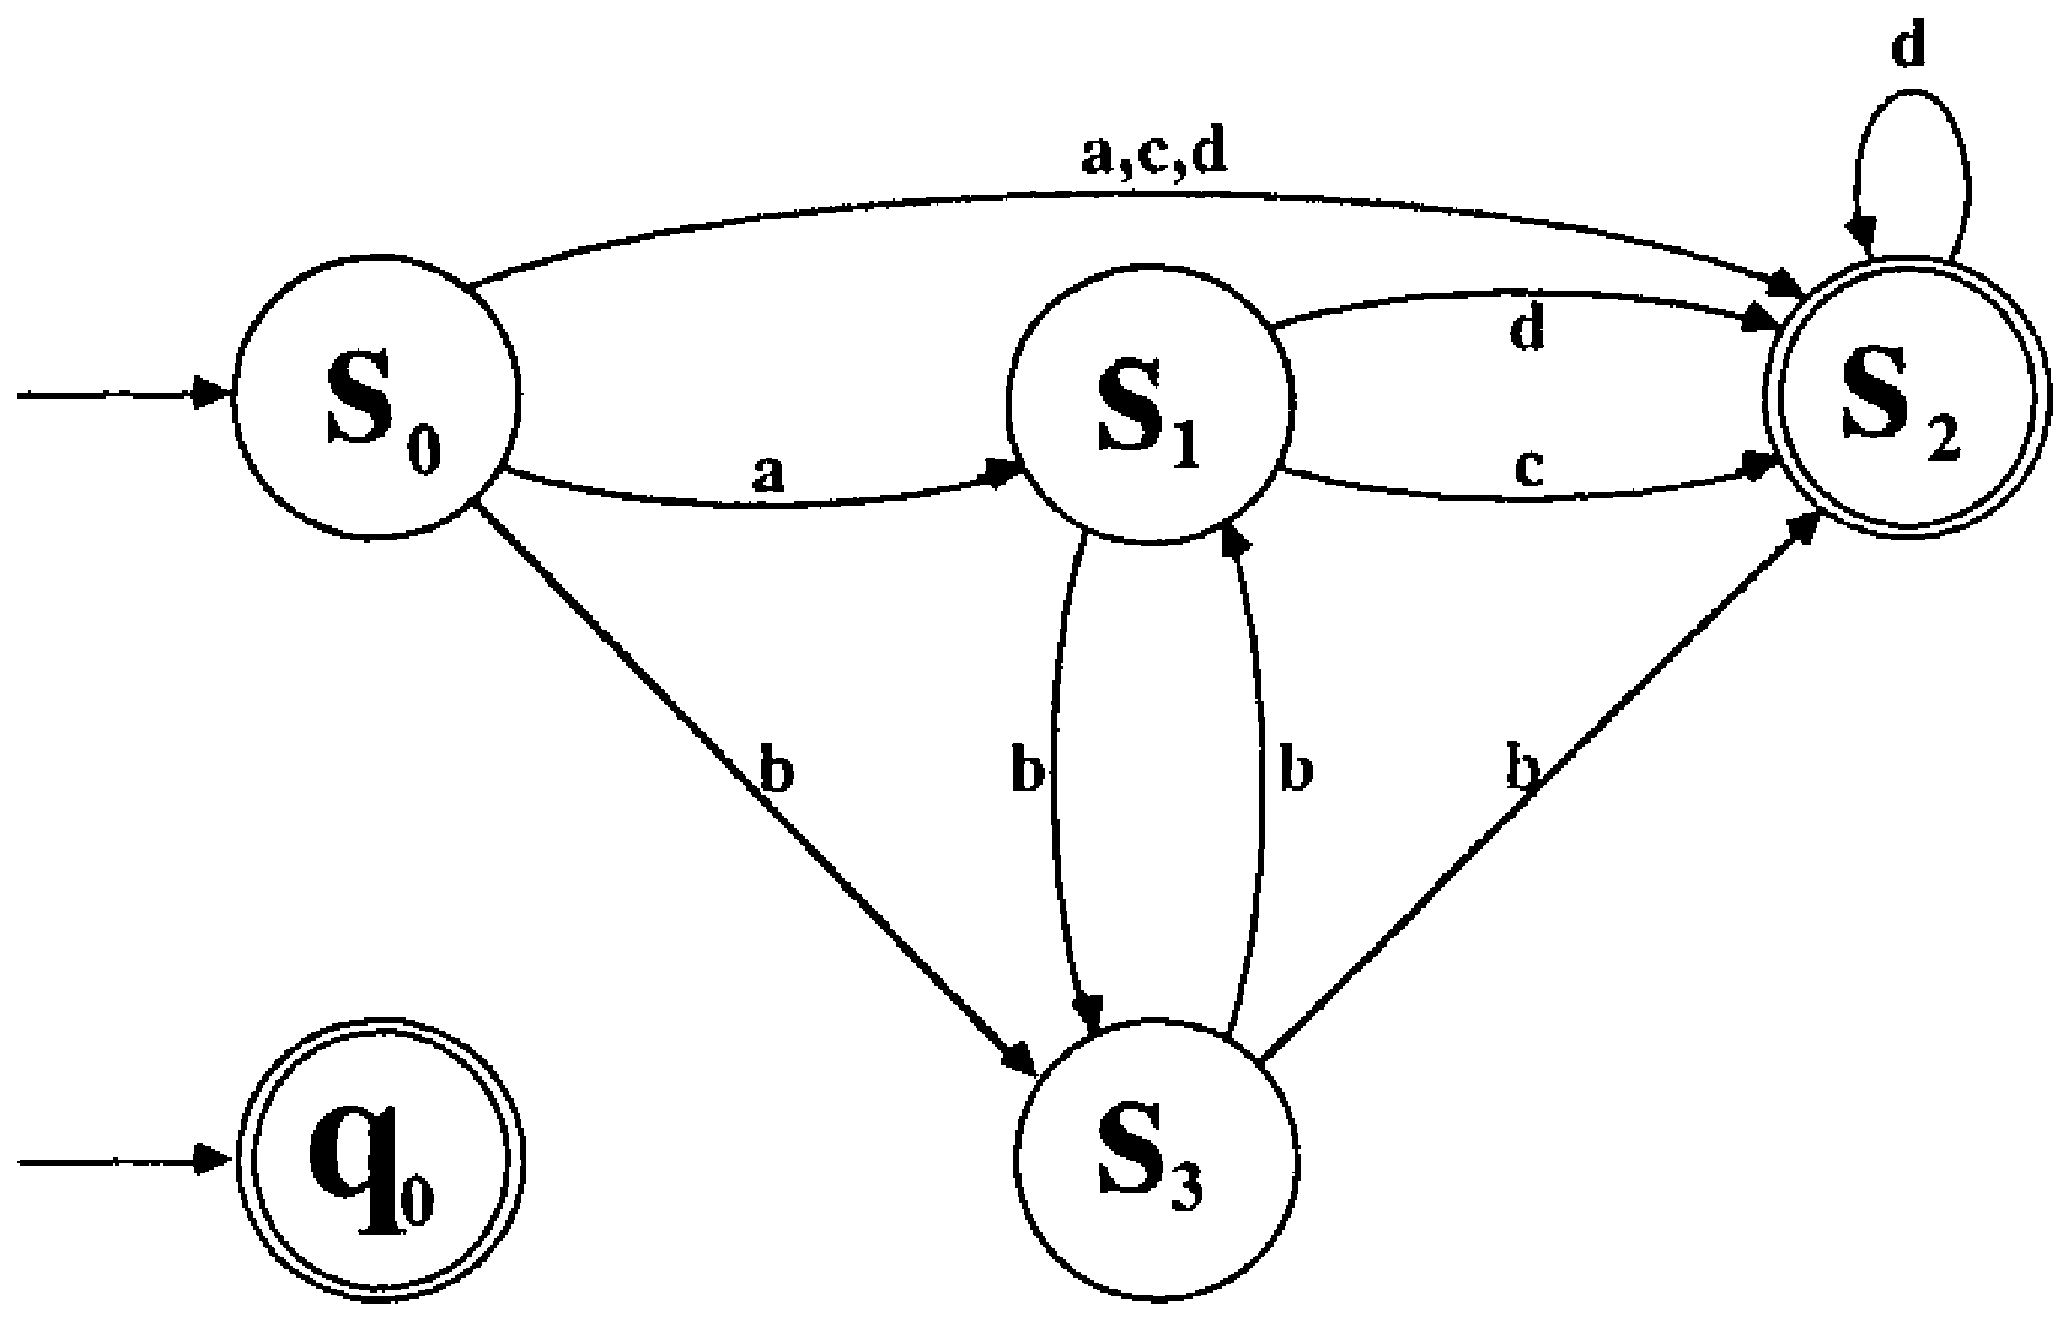
\epsfig{figure=ToFAfigures/fig4-20.eps,width=3.5in}}
\caption{An NDFA without lambda-moves that is equivalent to the automaton in
Figure \ref{fig-4.19}}\label{fig-4.20}
\end{figure}

% Definition 4.9
\begin{dfn}\label{dfn-4.9}
Given a nondeterministic finite automaton \emph{with} $\lambda$-transitions,
$A_{\lambda}=\langle\Sigma,S,S_0,\delta_{\lambda},F\rangle$, the
\emph{corresponding nondeterministic finite automaton without
$\lambda$-transitions}, $A^{\sigma}_{\lambda}=\langle\Sigma,S\cup\{q_0\},S_0\cup
\{q_0\},\delta^{\sigma}_{\lambda},F^{\sigma}\rangle$, is defined as follows:

\begin{center}\begin{tabular}{l}
$F^{\sigma} = \left\{ \begin{tabular}{ll}
		$F$ & $\quad\text{iff}\quad\lambda\notin L(A_{\lambda})$ \\
 		$F \cup \{q_0\}$ & $\quad\text{iff}\quad \lambda\in
			L(A_{\lambda})$
		\end{tabular}\right. $ \\
$(\forall\pmb{a}\in\Sigma)\delta^{\sigma}_{\lambda}(q_0,\pmb{a}) = \emptyset$ \\
$(\forall s \in S)(\forall\pmb{a}\in\Sigma)\quad \delta^{\sigma}_{\lambda}(s,
	\pmb{a}) = \DBAR_{\!\lambda}(s,\pmb{a}) =
        \Lambda(\bigcup\limits_{q\,\in\,\Lambda(s)}\delta_{\lambda}
	(q,\pmb{a}))$
\end{tabular}\end{center}
and which is extended in the ``usual'' way for nondeterministic finite automata
to the function \linebreak$\overline{\delta^{\sigma}_{\lambda}}$$: (S \cup \{q_0\}) \times \Sigma^*
\rightarrow \wp(S \cup \{q_0\})$.
\end{dfn}

Note that from a state in $A_{\lambda}$ several $\lambda$-transitions may be
taken, then a single letter $\pmb{a}$ may be processed, and then several more
$\lambda$-moves may occur; all this activity can result from just a single
symbol on the input tape being processed. The definition of
$\delta^{\sigma}_{\lambda}$ reflects these types of transitions. The
$\delta^{\sigma}_{\lambda}$ function is defined to be the same as the
$\DBAR_{\lambda}$ function for all single letters (strings of length 1), which
adjusts for the $\lambda$-closure of $A_{\lambda}$. The
$\delta^{\sigma}_{\lambda}$ function can then be extended in the usual
nondeterministic manner.

To account for the case that $\lambda$ might be in the language accepted by the
automaton $A_{\lambda}$, we add an extra start state $q_0$ to the corresponding
machine $A^{\sigma}_{\lambda}$, which is disconnected from the rest of the
machine. If $\lambda\in L(A_{\lambda})$, we also make $q_0$ a final state.

\subsection*{Example 4.15}

Let $A_{\lambda}$ represent the NDFA given in Example 4.14. $A^{\sigma}_{\lambda}$ would
then be given by the NDFA shown in Figure \ref{fig-4.20}. This new NDFA does indeed accept
the same language as $A_{\lambda}$. To show in general that $L(A_{\lambda}) =
L(A^{\sigma}_{\lambda})$, we must first show that the respective extended state
transition functions behave in similar fashions. However, these two functions
can be equivalent only for strings of nonzero length (because of the effects of
the $\lambda$-closure in the definition of $\delta^{\sigma}_{\lambda}$). This
result is established in Lemma \ref{lmm-4.2}.

% Lemma 4.2
\begin{lmm}\label{lmm-4.2}
Given a nondeterministic finite automaton $A_{\lambda}$ \emph{with}
$\lambda$-transitions and the corresponding nondeterministic finite automaton
$A^{\sigma}_{\lambda}$ \emph{without} $\lambda$-transitions, then
\[ (\forall s \in S)(\forall x \in \Sigma^+)(\overline{\delta^{\sigma}_{\lambda}}(s,x) =
	\DBAR_{\lambda}(s,x)) \]
\emph{Proof.} The proof is by induction on $|x|$; see the exercises.
\end{lmm}

Once we have shown that the extended state transition functions behave
(almost) identically, we can proceed to show that the languages accepted by
these two machines are the same.

% Theorem 4.2
\begin{thm}\label{thm-4.2}\index{equivalent!NDFAs}
Given a nondeterministic finite automaton that contains $\lambda$-transitions,
there exists an \emph{equivalent} nondeterministic finite automaton that does
not have $\lambda$-transitions.

\emph{Proof.} Assume $A_{\lambda}=\langle\Sigma,S,S_0,\delta_{\lambda},F\rangle$
is an NDFA with $\lambda$-transitions. Construct the corresponding NDFA
$A^{\sigma}_{\lambda} = \langle\Sigma,S\cup\{q_0\},S_0\cup\{q_0\},
\delta^{\sigma}_{\lambda},F^{\sigma}\rangle$, which has no $\lambda$-transitions.
We will show $L(A_{\lambda})=L(A^{\sigma}_{\lambda})$, and thereby prove that the
two machines are equivalent. Because the way $A^{\sigma}_{\lambda}$ was constructed
limits the scope of Lemma \ref{lmm-4.2}, the proof is divided into two cases.

{\bf Case 1}: If $x = \lambda$, then by Definition \ref{dfn-4.9}
\[ (q_0 \in F^{\sigma}\text{ iff }\lambda \in L (A_{\lambda})) \]
and so
\[ (\lambda \in L(A^{\sigma}_{\lambda}) \Leftrightarrow \lambda \in
	L(A_{\lambda})) \]

{\bf Case 2}: Assume $x \neq \lambda$. Since there are no transitions leaving
$q_0$, it may be disregarded as one of the start states of $A^{\sigma}_{\lambda}$. Then
\begin{center}\begin{tabular}{rcl}
$x \in L(A^{\sigma}_{\lambda})$ & $\Rightarrow$ & (by definition of $L$) \\
$(\bigcup\limits_{s_0\,\in\, S_0}\overline{\delta^{\sigma}_{\lambda}}(s_0,x)) \cap F^{\sigma}
	\not=\emptyset$ & $\Rightarrow$ & (by Lemma \ref{lmm-4.2}) \\
$(\bigcup\limits_{s_0\,\in\, S_0}\DBAR_{\lambda}(s_0,x)) \cap F^{\sigma} \not=
	\emptyset$ & $\Rightarrow$ & \begin{tabular}{l}(since if $q_0$ were the
	common element, then $x$ \\ would have to be $\lambda$, which violates
	the assumption) \end{tabular} \\
$(\bigcup\limits_{s_0\,\in\, S_0}\DBAR_{\lambda}(s_0,x)) \cap F \not= \emptyset$
	& $\Rightarrow$ & (by definition of $L$)
\\$x \in L(A_{\lambda})$
\end{tabular}\end{center}
Conversely, and for many of the same reasons, we have
\begin{center}\begin{tabular}{rcl}
$x \in L(A_{\lambda})$ & $\Rightarrow$ & (by definition of $L$) \\
$(\bigcup\limits_{s_0\,\in\, S_0}\DBAR_{\lambda}(s_0,x)) \cap F \not= \emptyset$
	& $\Rightarrow$ & (by Lemma \ref{lmm-4.2}) \\
$(\bigcup\limits_{s_0\,\in\, S_0}\overline{\delta^{\sigma}_{\lambda}}(s_0,x)) \cap F
	\not=\emptyset$ & $\Rightarrow$ & (since $F \subseteq F^{\sigma}$) \\
$(\bigcup\limits_{s_0\,\in\, S_0}\overline{\delta^{\sigma}_{\lambda}}(s_0,x)) \cap F^{\sigma}
	\not=\emptyset$ & $\Rightarrow$ & (by definition of $L$) \\
$x \in L(A^{\sigma}_{\lambda})$ &&
\end{tabular}\end{center}
Consequently, $(\forall x \in \Sigma^*)(x \in L(A^{\sigma}_{\lambda})
\Leftrightarrow x \in L(A_{\lambda}))$.
\end{thm}

Although nondeterministic finite automata \emph{with} $\lambda$-transitions are
no more powerful than nondeterministic finite automata \emph{without}
$\lambda$-transitions and consequently recognize the same class of languages as
deterministic finite automata, they have their place in theory and machine
construction. Because such machines can be constructed very easily from
\emph{regular expressions} (see Chapter \ref{ch-6}), NDFAs are used by the
UNIX$^{\text{TM}}$ text editor and by lexical analyzer generators such as LEX for
pattern-matching applications. Example 4.16 involves the regular expression
$(\pmb{a}\cup\pmb{c})^*\pmb{bc}(\pmb{a}\cup\pmb{c})^*$, which describes the set
of words composed of any number of $\pmb{a}$s and $\pmb{c}$s, followed by a single
$\pmb{b}$, followed by a single $\pmb{c}$, followed by any number of $\pmb{a}$s and
$\pmb{c}$s.

\subsection*{Example 4.16}

Suppose that we wanted to construct a machine that will accept the language
$L=\{x \in \{\pmb{a},\pmb{b},\pmb{c}\}^*|x$ contains exactly one $\pmb{b}$, which
is immediately followed by $\pmb{c}\}$. A machine that accepts this language is
given in Figure \ref{fig-4.21}.

% Figure 4.21
\begin{figure}
\centerline{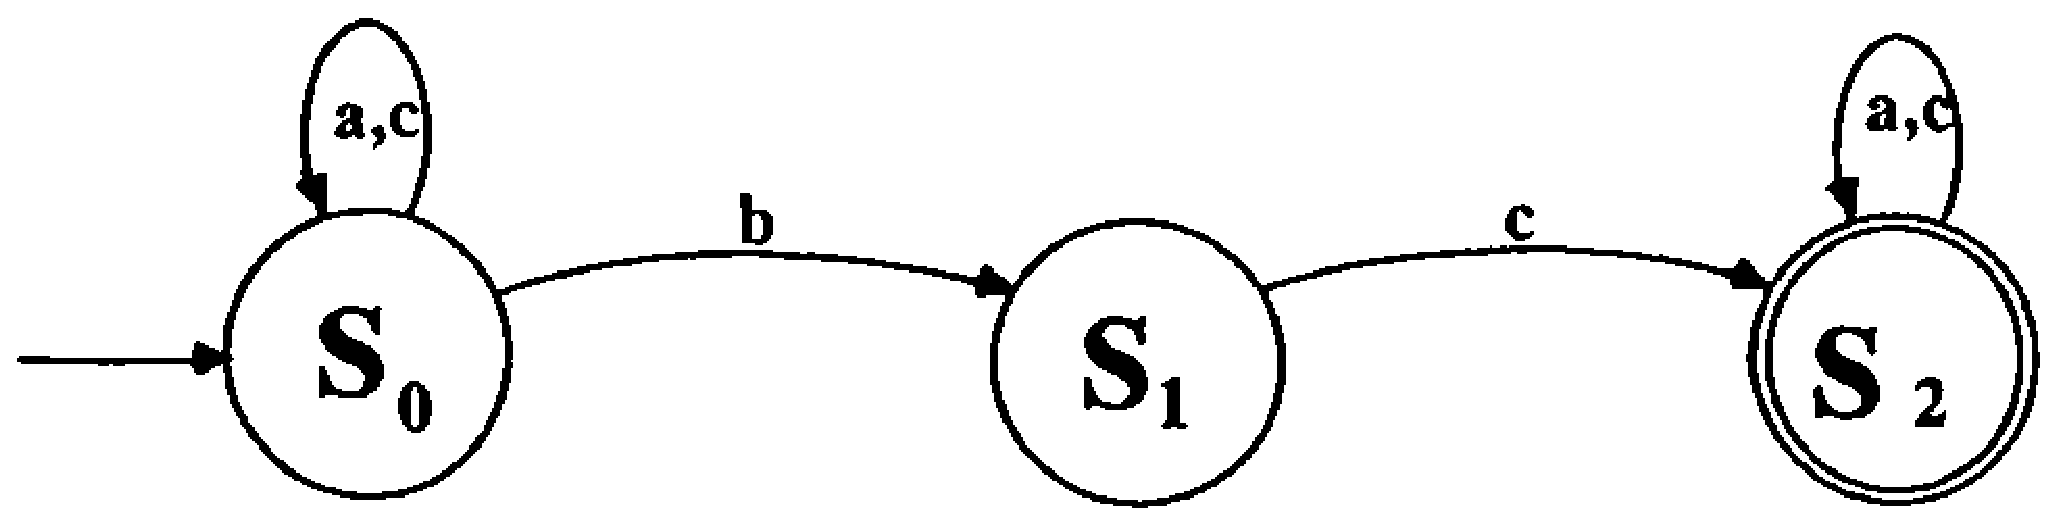
\epsfig{figure=ToFAfigures/fig4-21.eps,width=3.0in}}
\caption{The NDFA described in Example 4.16}\label{fig-4.21}
\end{figure}

Suppose we now wish to build a machine that will accept any positive number of
occurrences of various strings from this language concatenated together. In this
case, the resulting language would include all strings (with at least one $\pmb{
b}$) with the property that each and every $\pmb{b}$ is immediately followed by
$\pmb{c}$. By simply adding a $\lambda$-transition from every final state to the
start state, we achieve our objective. The machine that accepts this new
language is shown in Figure \ref{fig-4.22}.

% Figure 4.22
\begin{figure}
\centerline{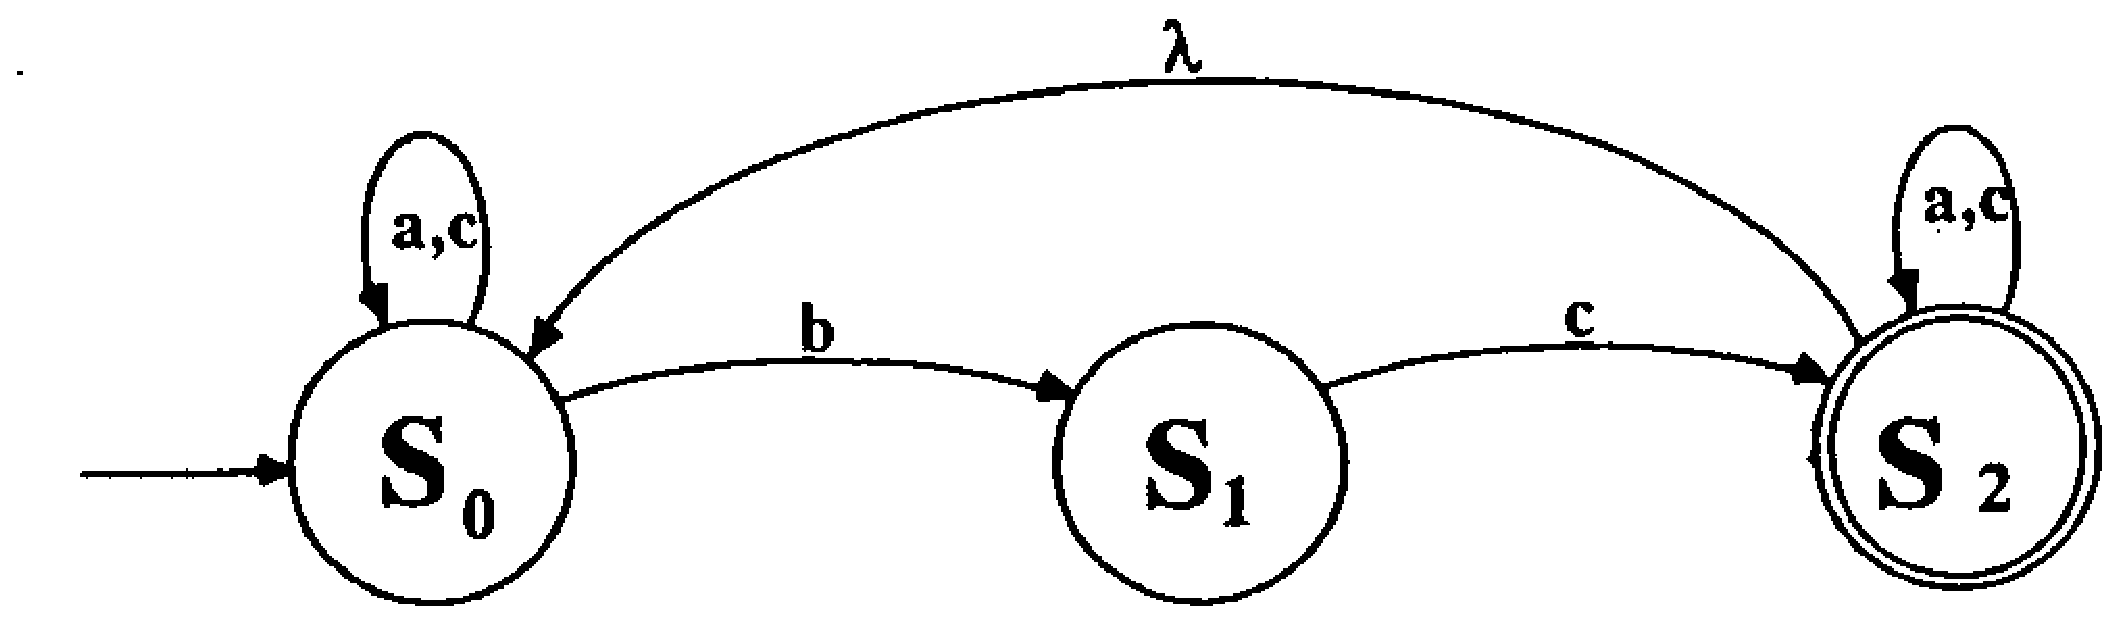
\epsfig{figure=ToFAfigures/fig4-22.eps,width=3.0in}}
\caption{The modification of the NDFA in Figure \ref{fig-4.21}}\label{fig-4.22}
\end{figure}

The previous section outlined how to implement nondeterministic finite automata
\emph{without} $\lambda$-transitions; accommodating $\lambda$-moves is in fact
quite straightforward. A $\lambda$-transition from state $s$ to state $t$
indicates that state $t$ should be considered active whenever state $s$ is
active. This can be assured by an obvious modification, as shown by the
following example.

% Figure 4.23
\begin{figure}
\centerline{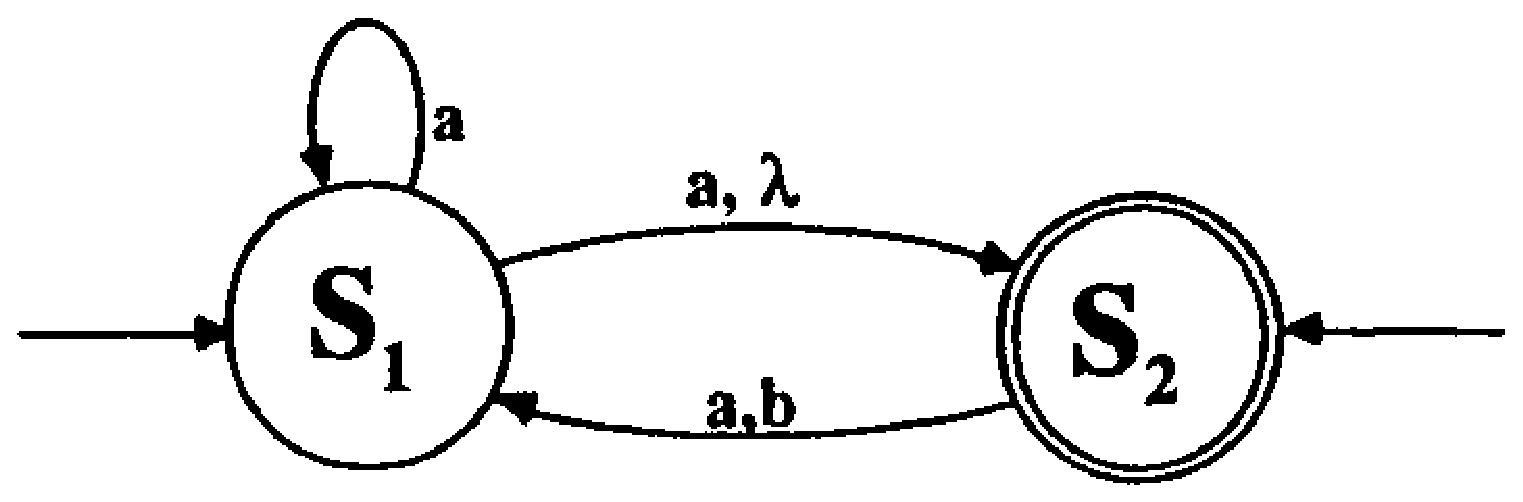
\epsfig{figure=ToFAfigures/fig4-23.eps,width=3.0in}}
\caption{A simple NDFA with lambda moves}\label{fig-4.23}
\end{figure}

\subsection*{Example 4.17}

As an illustration of how circuitry can be defined for machines with
$\lambda$-transitions, consider the DFA $E$ given in Figure \ref{fig-4.23}. This machine
is similar to the NDFA $D$ in Example 4.13, but a $\lambda$-transition has been
added from $s_1$ to $s_2$; that is, $\delta(s_1,\lambda)=\{s_2\}$. This
transition implies that $s_2$ should be considered active whenever $s_1$ is
active. Consequently, the circuit diagram produced in Example 4.13 need only be
slightly modified by establishing the extra connection indicated by the dotted
line shown in Figure \ref{fig-4.24}.

In general, the need for such ``extra'' connections leaving a given flip-flop
input $t_i$ is determined by examining $\delta(s_i,\lambda)$, the set of
$\lambda$-transitions for $s_i$. Note that the propagation delay in this circuit
has been increased; there are signals that must now propagate through an extra
gate during a single clock cycle. The delay will be exacerbated in automata that
contain sequences of $\lambda$-transitions. In such cases, the length of the
clock cycle may need to be increased to ensure proper operation. This problem
can be minimized by adding all the connections indicated by $\Lambda(s_i)$,
rather than just adding those implied by $\delta(s_i,\lambda)$.

% Figure 4.24
\begin{figure}
\centerline{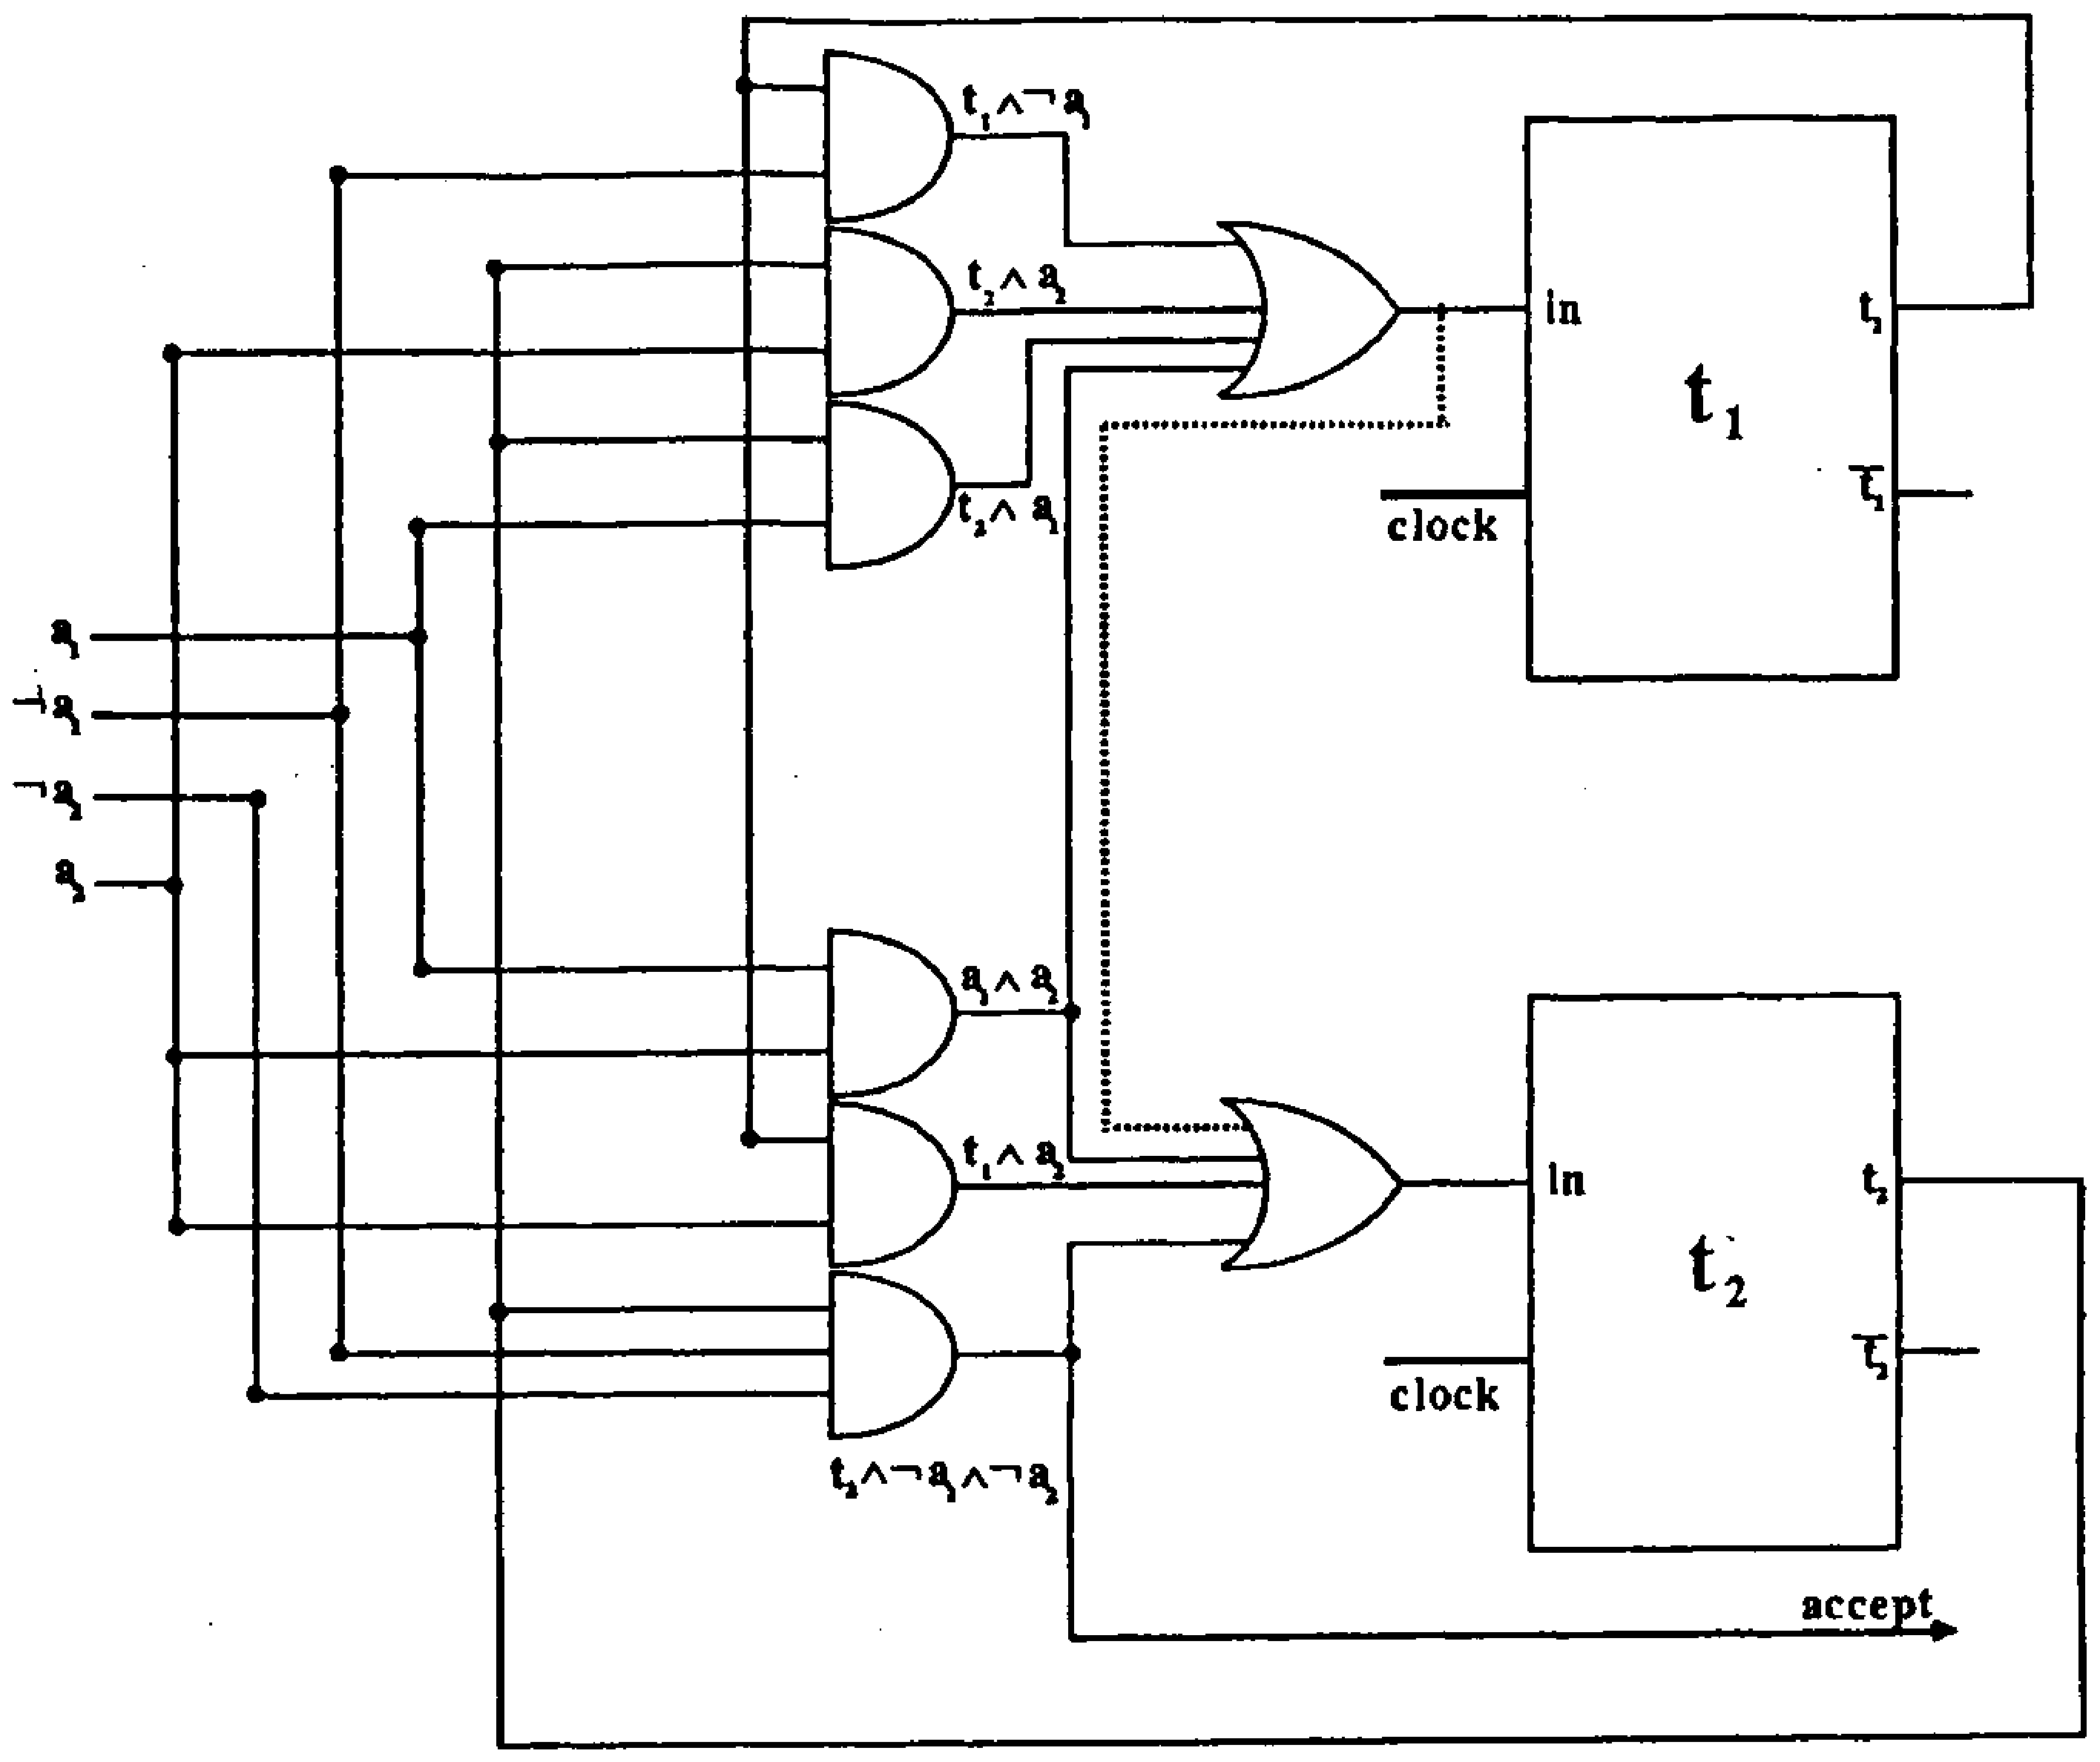
\epsfig{figure=ToFAfigures/fig4-24.eps,width=6.0in}}
\caption{Circuitry for the automaton discussed in Example 4.17}\label{fig-4.24}
\end{figure}

\section*{Exercises}
\begin{enumerate}[{4.}1.]
\item Draw the deterministic versions of each of the nondeterministic finite
automata shown in Figure \ref{fig-4.25}. In each part, assume $\Sigma=\{\pmb{a},\pmb{b},
\pmb{c}\}$.

\item Consider the automaton given in Example 4.17.
\begin{enumerate}
\item Convert this automaton into an NDFA without $\lambda$-transitions using
Definition \ref{dfn-4.9}.
\item Convert this NDFA into a DFA using Definition \ref{dfn-4.5}.
\end{enumerate}

% Figure 4.25
\begin{figure}
\centerline{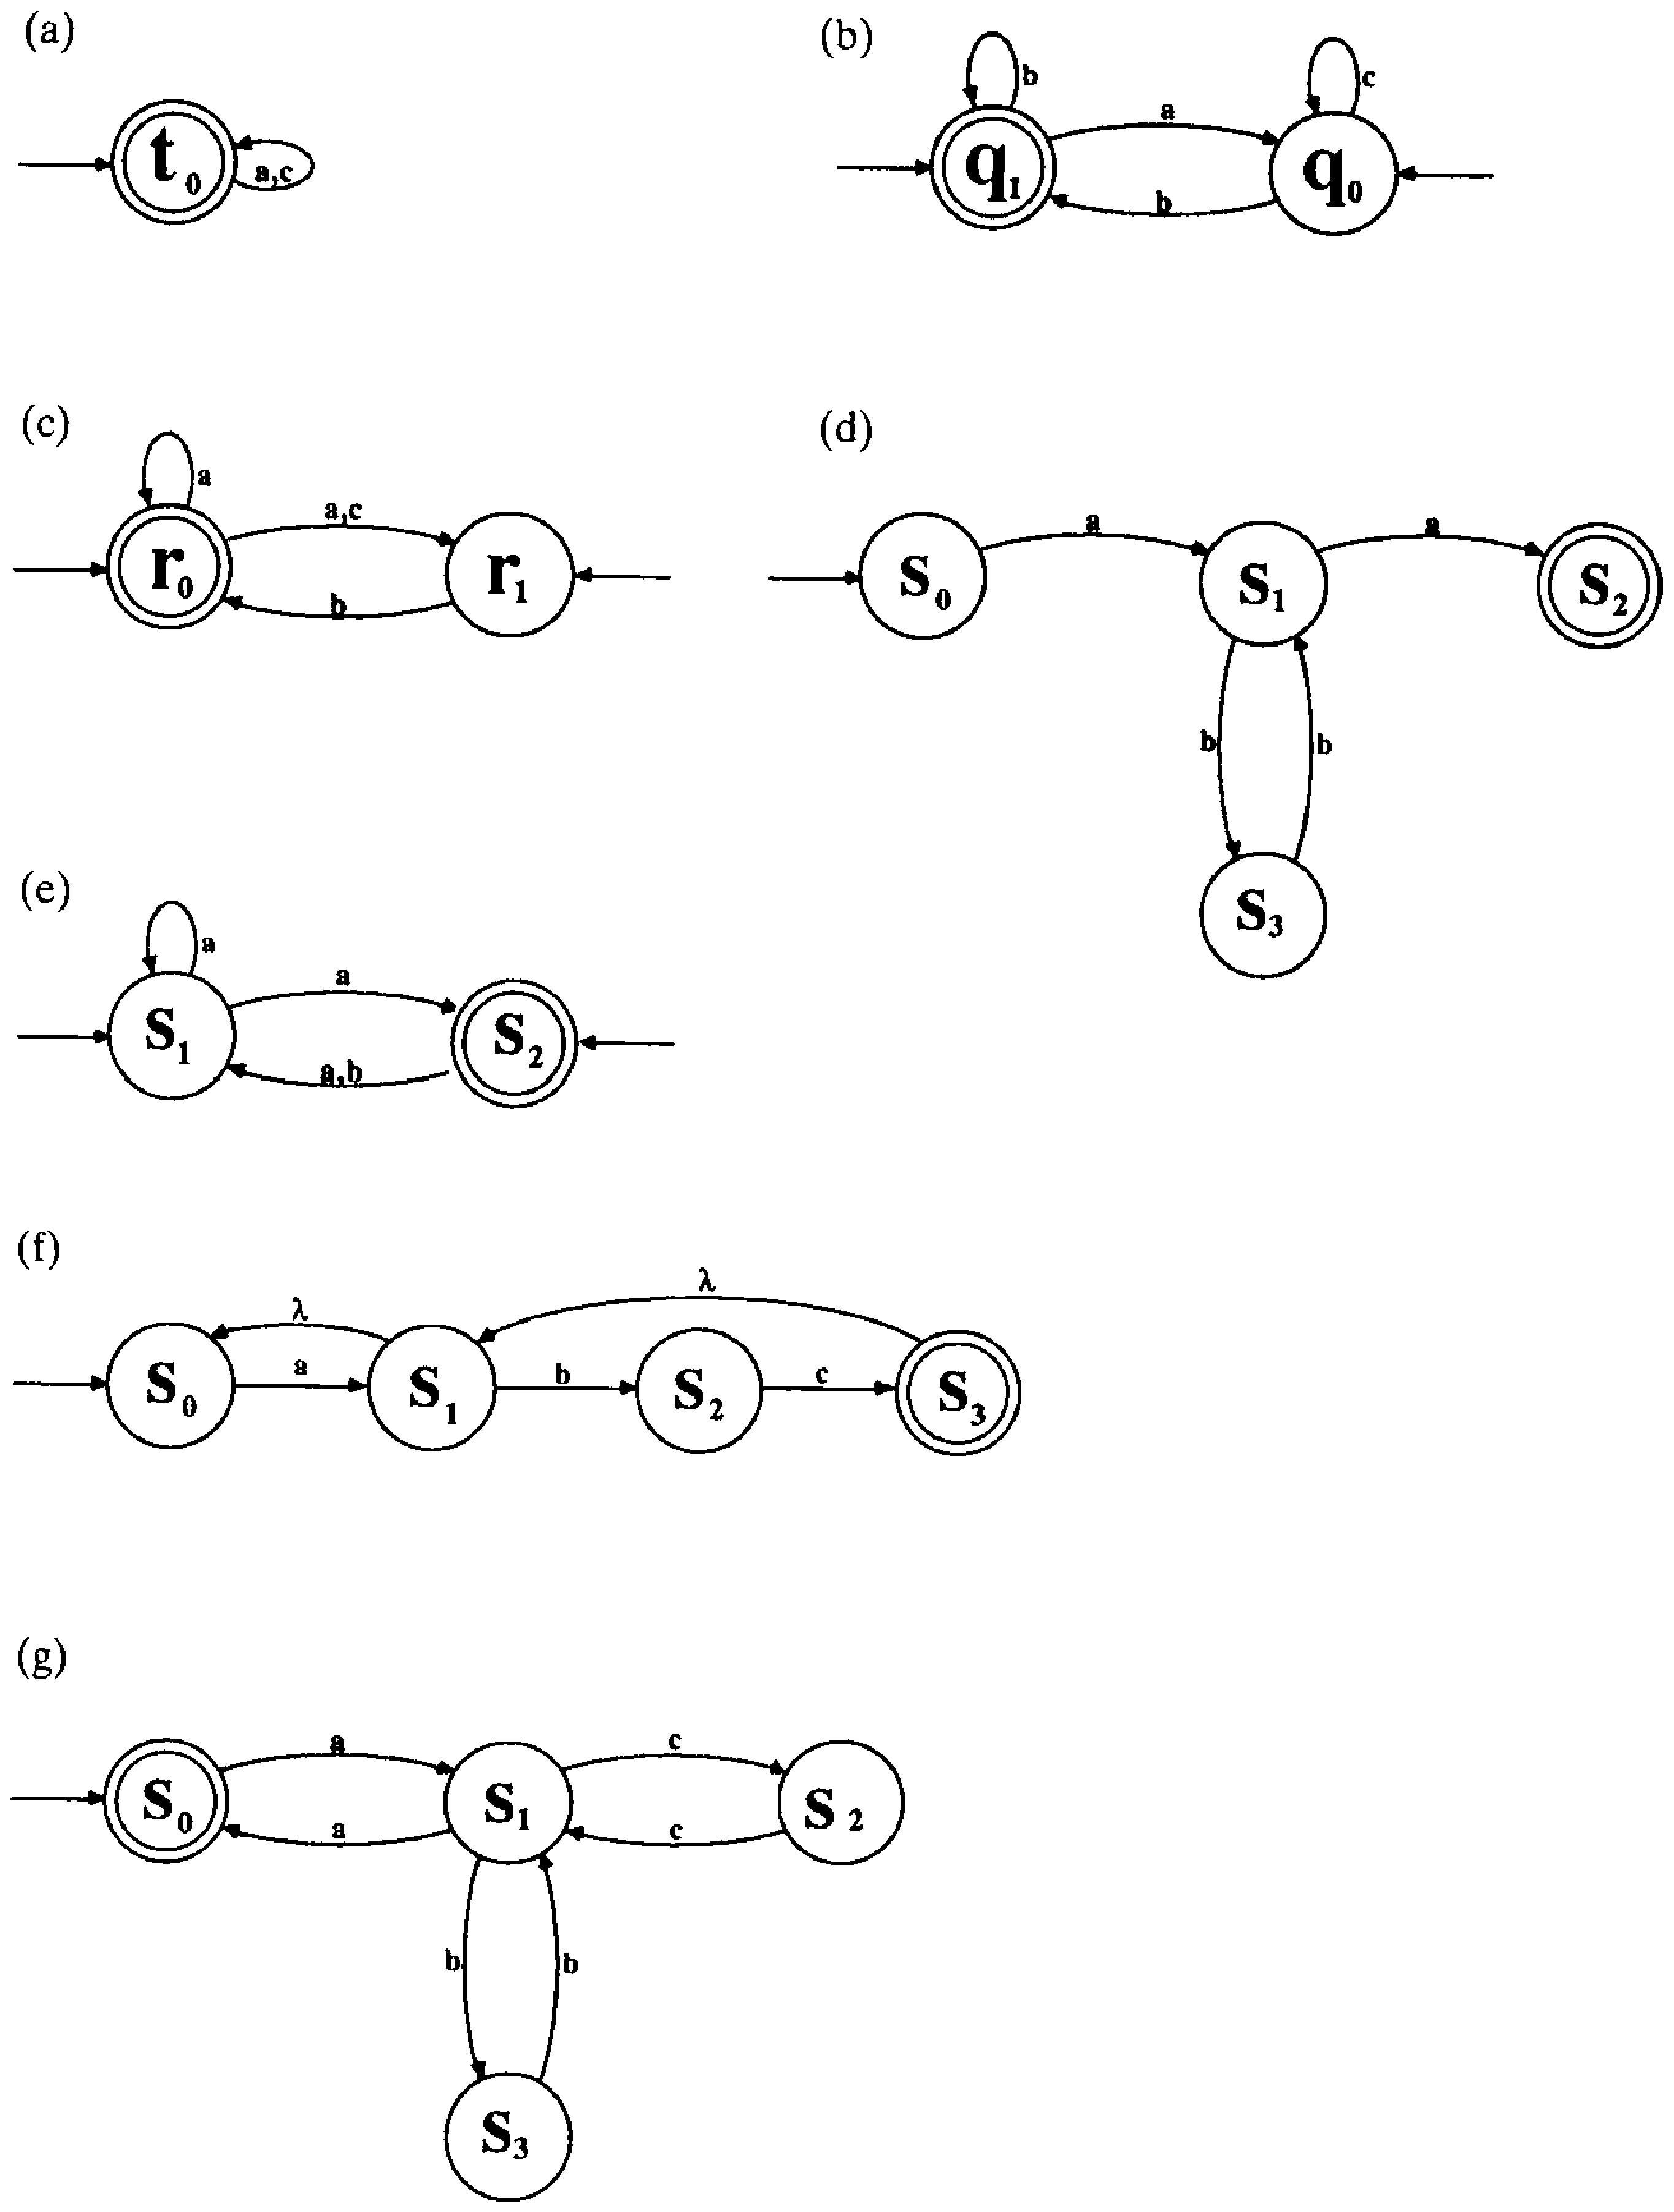
\epsfig{figure=ToFAfigures/fig4-25.eps,width=6.0in}}
\caption{Automata for Exercise 4.1}\label{fig-4.25}
\end{figure}

\item Consider the automaton given in Example 4.4.
\begin{enumerate}
\item Using the standard encodings, draw a circuit diagram for this NDFA
(include neither \<SOS\> nor \<EOS\>)
\item Using the standard encodings, draw a circuit diagram for this NDFA
(include both \<SOS\> and \<EOS\>)
\item Convert the NDFA into a DFA using Definition \ref{dfn-4.5} (draw only the connected
portion of the machine).
\item Convert the NDFA into a DFA using Definition \ref{dfn-4.5} (draw the entire machine,
including the disconnected portion).
\end{enumerate}

\item Consider the automaton given in Example 4.2.
\begin{enumerate}
\item Using the standard encodings, draw a circuit diagram for this NDFA
(include both \<SOS\> and \<EOS\>)
\item Convert the NDFA into a DFA using Definition \ref{dfn-4.5}.
\end{enumerate}

\item Consider the automaton given in Example 4.3.
\begin{enumerate}
\item Using the standard encodings, draw a circuit diagram for this NDFA
(include neither \<SOS\> nor \<EOS\>).
\item Using the standard encodings, draw a circuit diagram for this NDFA
(include both \<SOS\> and \<EOS\>)
\item Convert the NDFA into a DFA using Definition \ref{dfn-4.5} (draw only the connected
portion of the machine).
\item Is this DFA isomorphic to any of the automata constructed in Exercise 4.4?
\end{enumerate}

\item Consider the automaton given in Example 4.14.
\begin{enumerate}
\item Using the standard encodings, draw a circuit diagram for this NDFA
(include neither \<SOS\> nor \<EOS\>)
\item Using the standard encodings, draw a circuit diagram for the NDFA in part
(b) (include neither \<SOS\> nor \<EOS\>)
\end{enumerate}

\item Consider the automaton given in the second part of Example 4.16.
\begin{enumerate}
\item Using the standard encodings, draw a circuit diagram for this NDFA
(include \<EOS\> but not \<SOS\>)
\item Build the equivalent automaton \emph{without} $\lambda$-transitions using
Definition \ref{dfn-4.9}.
\item Using the standard encodings, draw a circuit diagram for the NDFA in part
(b) (include \<EOS\> but not \<SOS\>)
\item Convert the NDFA into a DFA using Definition \ref{dfn-4.5} (draw only the connected
portion of the machine).
\end{enumerate}

\item It is possible to build a \emph{deterministic finite automaton}
$\overline{A}$ such that the language accepted by this machine is the
\emph{absolute complement} of the language accepted by a machine $A$ [that is,
$L(\overline{A})=\Sigma^* - L(A)$] by simply complementing the set of final
states (see Theorem \ref{thm-5.1}). Can a similar thing be done for nondeterministic
finite automata? If not, why not? Give an example to support your statements.

\item Given a nondeterministic finite automaton $A$ \emph{without}
$\lambda$-transitions, show that it is possible to construct a nondeterministic
finite automaton \emph{with} $\lambda$-transitions $A'$ with the properties
\begin{enumerate}[(1)]
\item $A'$ has exactly \emph{one} start state and exactly \emph{one} final state
and
\item $L(A') = L(A)$.
\end{enumerate}

\item Consider (ii) in Definition \ref{dfn-4.8}. Can this fact be deduced from parts (i)
and (iii)? Justify your answer.

\item If we wanted another way to construct a nondeterministic finite automaton
\emph{without} $\lambda$-transitions corresponding to one that does have them,
we could try the following: Let $S'=S,\ S'_0=\Lambda(S_0),\ F'=F$, and
$\delta'(s,\pmb{a})=\DBAR_{\lambda}(s,\pmb{a})$ for all $\pmb{a}\in\Sigma,s \in
S$. Show that this works (or if it does not work, explain why not and give an
example).

\item Using nondeterministic machines \emph{with} $\lambda$-transitions, give an
algorithm for constructing a $\lambda$-NDFA having \emph{one} start state and
\emph{one} final state that will accept the \emph{union} of two FAD languages.

\item Give an example of an NDFA $A$ for which:
\begin{enumerate}
\item $A^d$ is not connected.
\item $A^d$ is not reduced.
\item $A^d$ is minimal.
\end{enumerate}

\item Why was it necessary to include an ``extra'' state $q_0$ in the
construction of $A^{\sigma}_{\lambda}$ in Definition \ref{dfn-4.9}? Support your answer
with an example.

\item \begin{enumerate}
\item Using nondeterministic machines \emph{without} $\lambda$-transitions, give
an algorithm for constructing a machine that will accept the \emph{union} of two
languages.
\item Is this easier or more difficult than using machines \emph{with}
$\lambda$-transitions?
\item Is it possible to ensure that this machine \emph{both} (i) has exactly
\emph{one} start state \emph{and} (ii) has exactly \emph{one} final state?
\end{enumerate}

\item Consider the automaton $A^{\sigma}_{\lambda}$ given in Example 4.15.
\begin{enumerate}
\item Using the standard encodings, draw a circuit diagram for
$A^{\sigma}_{\lambda}$ (include neither \<SOS\> nor \<EOS\>)
\item Convert $A^{\sigma}_{\lambda}$ into $A^{\sigma d}_{\lambda}$ using
Definition \ref{dfn-4.5} (draw only the connected portion of the machine).
\end{enumerate}

\item \begin{enumerate}
\item Prove that for any NDFA \emph{without} $\lambda$-transitions the
definitions of \DBAR\ and $\delta$ agree for single letters; that is,
$(\forall s \in S)(\forall\pmb{a}\in\Sigma)(\DBAR(s,\pmb{a})=\delta(s,\pmb{a}))$.
\item Give an example to show that this need not be true for an NDFA \emph{with}
$\lambda$-transitions.
\end{enumerate}

\item Consider the NDFA that accepts the original language $L$ in Example 4.10.
\begin{enumerate}
\item Using the standard encodings, draw a circuit diagram for this NDFA
(include neither \<SOS\> nor \<EOS\>)
\item Convert the NDFA into a DFA using Definition \ref{dfn-4.5} (draw only the connected
portion of the machine).
\end{enumerate}

\item Consider the NDFA which accepts the modified language $L^r$ in Example
4.10.
\begin{enumerate}
\item Using the standard encodings, draw a circuit diagram for this NDFA
(include neither \<SOS\> nor \<EOS\>)
\item Convert the NDFA into a DFA using Definition \ref{dfn-4.5} (draw only the connected
portion of the machine).
\end{enumerate}

\item Consider the arguments leading up to the pumping lemma in Chapter \ref{ch-2}. Are
they still valid when applied to NDFAs?

\item Consider Theorem \ref{thm-2.7}. Does the conclusion still hold if applied to an
NDFA?

\item Given a nondeterministic finite automaton $A$ (without
$\lambda$-transitions) for which $\lambda \notin L(A)$, show that it is possible
to construct a nondeterministic finite automaton (also without
$\lambda$-transitions) $A''$ with the properties:
\begin{enumerate}[1.]
\item $A''$ has exactly \emph{one} start state.
\item $A''$ has exactly \emph{one} final state.
\item $L(A'') = L(A)$.
\end{enumerate}

\item Give an example to show that if $\lambda \in L(A)$ it may not be possible
to construct an NDFA without $\lambda$-transitions satisfying all three
properties listed in Exercise 4.22.

\item Prove Lemma \ref{lmm-4.2}.

\item Given a DFA $A$, show that it can be thought of as an NDFA $A^n$ and that,
furthermore, $L(A^n) = L(A)$. \emph{Hint:} Carefully define your ``new'' machine
$A^n$, justify that it is indeed an NDFA, make the appropriate inductive
statement, and argue that $L(A^n) = L(A)$.

\item Give an example to show that the domain of Lemma \ref{lmm-4.2} cannot be expanded
to include $\lambda$; that is, show that $\overline{\delta^{\sigma}_{\lambda}}(s,\lambda)
\not= \DBAR_{\lambda}(s,\lambda)$.

\item Refer to Definition \ref{dfn-4.5} and prove the fact used in Lemma \ref{lmm-4.1}:
\[ (\forall A \in \wp(S))(\forall B \in \wp(S))(\forall\pmb{a}\in\Sigma)(\delta^d
	(A \cup B,\pmb{a}) = \delta^d(A,\pmb{a}) \cup \delta^d(B,\pmb{a})) \]
	
\item Recall that if a word can reach several states in an NDFA, some of which
are final and some nonfinal, Definition \ref{dfn-4.4} requires us to accept that word.
\begin{enumerate}
\item Change the definition of $L(A)$ so that a word is accepted only if
\emph{every} state the word can reach is final.
\item Change the definition of $A^d$ to produce a deterministic machine that
accepts only those words specified in part (a).
\end{enumerate}

\item Draw the connected part of $T^d$,the deterministic equivalent of the NDFA
$T$ in Example 4.7.

\item Refer to Example 4.7 and modify the NDFA $T$ so that the machine reverts
to a nonfinal state (that is, turns the recorder off) when the substring
$\pmb{000111}$ is detected. Note that $\pmb{000111}$ functions as the EOT (end
of transmission) signal.

\item Consider the automaton $A$ given in Example 4.14.
\begin{enumerate}
\item Draw a diagram of $A^{\sigma}_{\lambda}$.
\item Draw $A^{\sigma d}_{\lambda}$ (draw only the connected portion of the
machine).
\end{enumerate}

\item What is wrong with the following ``proof'' of Lemma \ref{lmm-4.2}? Let $P(k)$ be
defined by $P(k): (\forall s \in S)(\forall x \in \Sigma^k)
(\overline{\delta^{\sigma}_{\lambda}}(s,x)=\DBAR_{\lambda}(s,x))$. \\
\emph{Basis step} $(k = 1): (\forall s \in S)(\forall\pmb{a}\in\Sigma)
(\overline{\delta^{\sigma}_{\lambda}}(s,\pmb{a})=\delta^{\sigma}_{\lambda}(s,\pmb{a}) =
\DBAR_{\lambda}(s,\pmb{a}))$. \\
\emph{Inductive step}: Suppose that the result holds for all $x \in \Sigma^k$
and let $y \in \Sigma^{k+1}$. Then $(\exists x \in \Sigma^k)(\exists \pmb{a} \in
\Sigma \ni y = x\pmb{a})$. Then
\begin{center}\begin{tabular}{rcl}
$\overline{\delta^{\sigma}_{\lambda}}(s,y)$ & $=$ & $\overline{\delta^{\sigma}_{\lambda}}(s,x\pmb{a})$\\
& $=$ & $\delta^{\sigma}_{\lambda}(\overline{\delta^{\sigma}_{\lambda}}(s,x),\pmb{a})$ \\
& $=$ & $\overline{\delta^{\sigma}_{\lambda}}(\DBAR_{\lambda}(s,x),\pmb{a})$ \\
& $=$ & $\DBAR_{\lambda}(\DBAR_{\lambda}(s,x),\pmb{a})$ \\
& $=$ & $\DBAR_{\lambda}(s,x\pmb{a})$ \\
& $=$ & $\DBAR_{\lambda}(s,y)$
\end{tabular}\end{center}
Therefore, $P(k) \Rightarrow P(k + 1)$ for all $k \geq 1$, and by the principle
of mathematical induction, we are assured that the equation holds for all
$x \in \Sigma^+$.

\item Consider the automaton given in Example 4.7.
\begin{enumerate}
\item Using the standard encodings, draw a circuit diagram for this NDFA
(include neither \<SOS\> nor \<EOS\>)
\item Convert the NDFA into a DFA using Definition \ref{dfn-4.5} (draw only the connected
portion of the machine).
\end{enumerate}

\item Consider the automaton given in Example 4.11.
\begin{enumerate}
\item Using the standard encodings, draw a circuit diagram for this NDFA
(include neither \<SOS\> nor \<EOS\>)
\item Convert the NDFA into a DFA using Definition \ref{dfn-4.5} (draw only the connected
portion of the machine).
\end{enumerate}

\item Consider the automaton B given in Example 4.8.
\begin{enumerate}
\item Using the standard encodings, draw a circuit diagram for $B$ (include
neither \<SOS\> nor \<EOS\>).
\item Using the standard encodings, draw a circuit diagram for $B^d$ (include
neither \<SOS\> nor \<EOS\>). Encode the states in such a way that your circuit is similar
to the one found in part (a).
\end{enumerate}

\item Draw a circuit diagram for each NDFA given in Figure \ref{fig-4.25} (include
neither \<SOS\> nor \<EOS\>). Use the standard encodings.

\item Draw a circuit diagram for each NDFA given in Figure \ref{fig-4.25} (include both
\<SOS\> and \<EOS\>). Use the standard encodings.
(See Example 4.13 for the solution corresponding to Figure \ref{fig-4.25}e.)


\item Definition \ref{dfn-3.10} and the associated algorithms were used in Chapter \ref{ch-3} for
finding the connected portion of a DFA.
\begin{enumerate}
\item Adapt Definition \ref{dfn-3.10} so that it applies to NDFAs.
\item Prove that there is an algorithm for finding the connected portion of an
NDFA.
\end{enumerate}
\end{enumerate}
